% !Mode:: "TeX:UTF-8"
% !TEX root = ..\thesis.tex
\chapter{实验结果图表}
模型1 和模型2 运用其相应的不同算法得到了目标函数值、流水线均衡率等结果,图表可以让不同算法的对比显得直观。不同决策参数$\lambda_1$、流水线数量$m$及订单数量$n$的环境下,模型1 的所得结果如\reff{fig:result1} -- \reff{fig:result3}所示,模型2 的所得结果如\reff{fig:result4} -- \reff{fig:result9}所示。
\begin{sidewaysfigure}
\centering
\subfloat[$n = 20$]{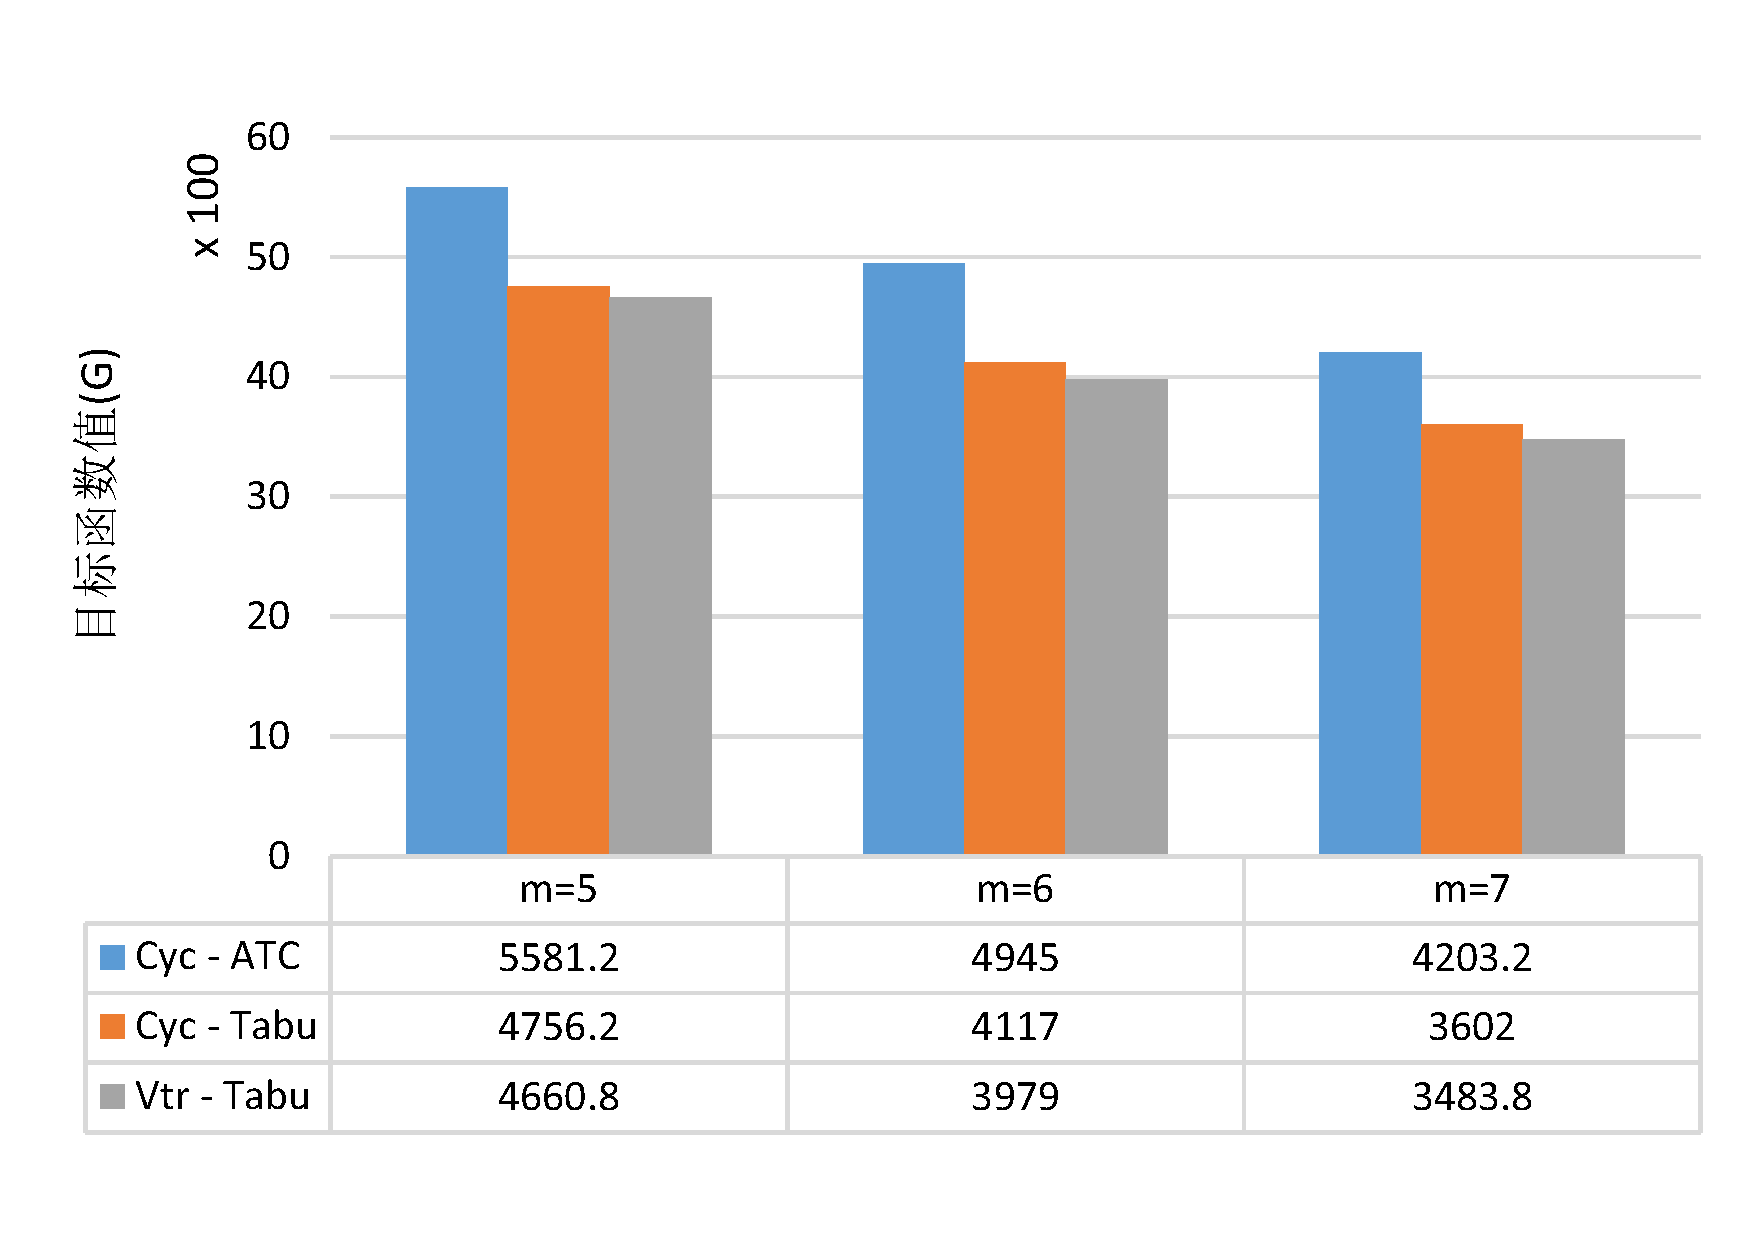
\includegraphics[height = 6cm, angle = -90]{basic_04_20}}
\subfloat[$n = 30$]{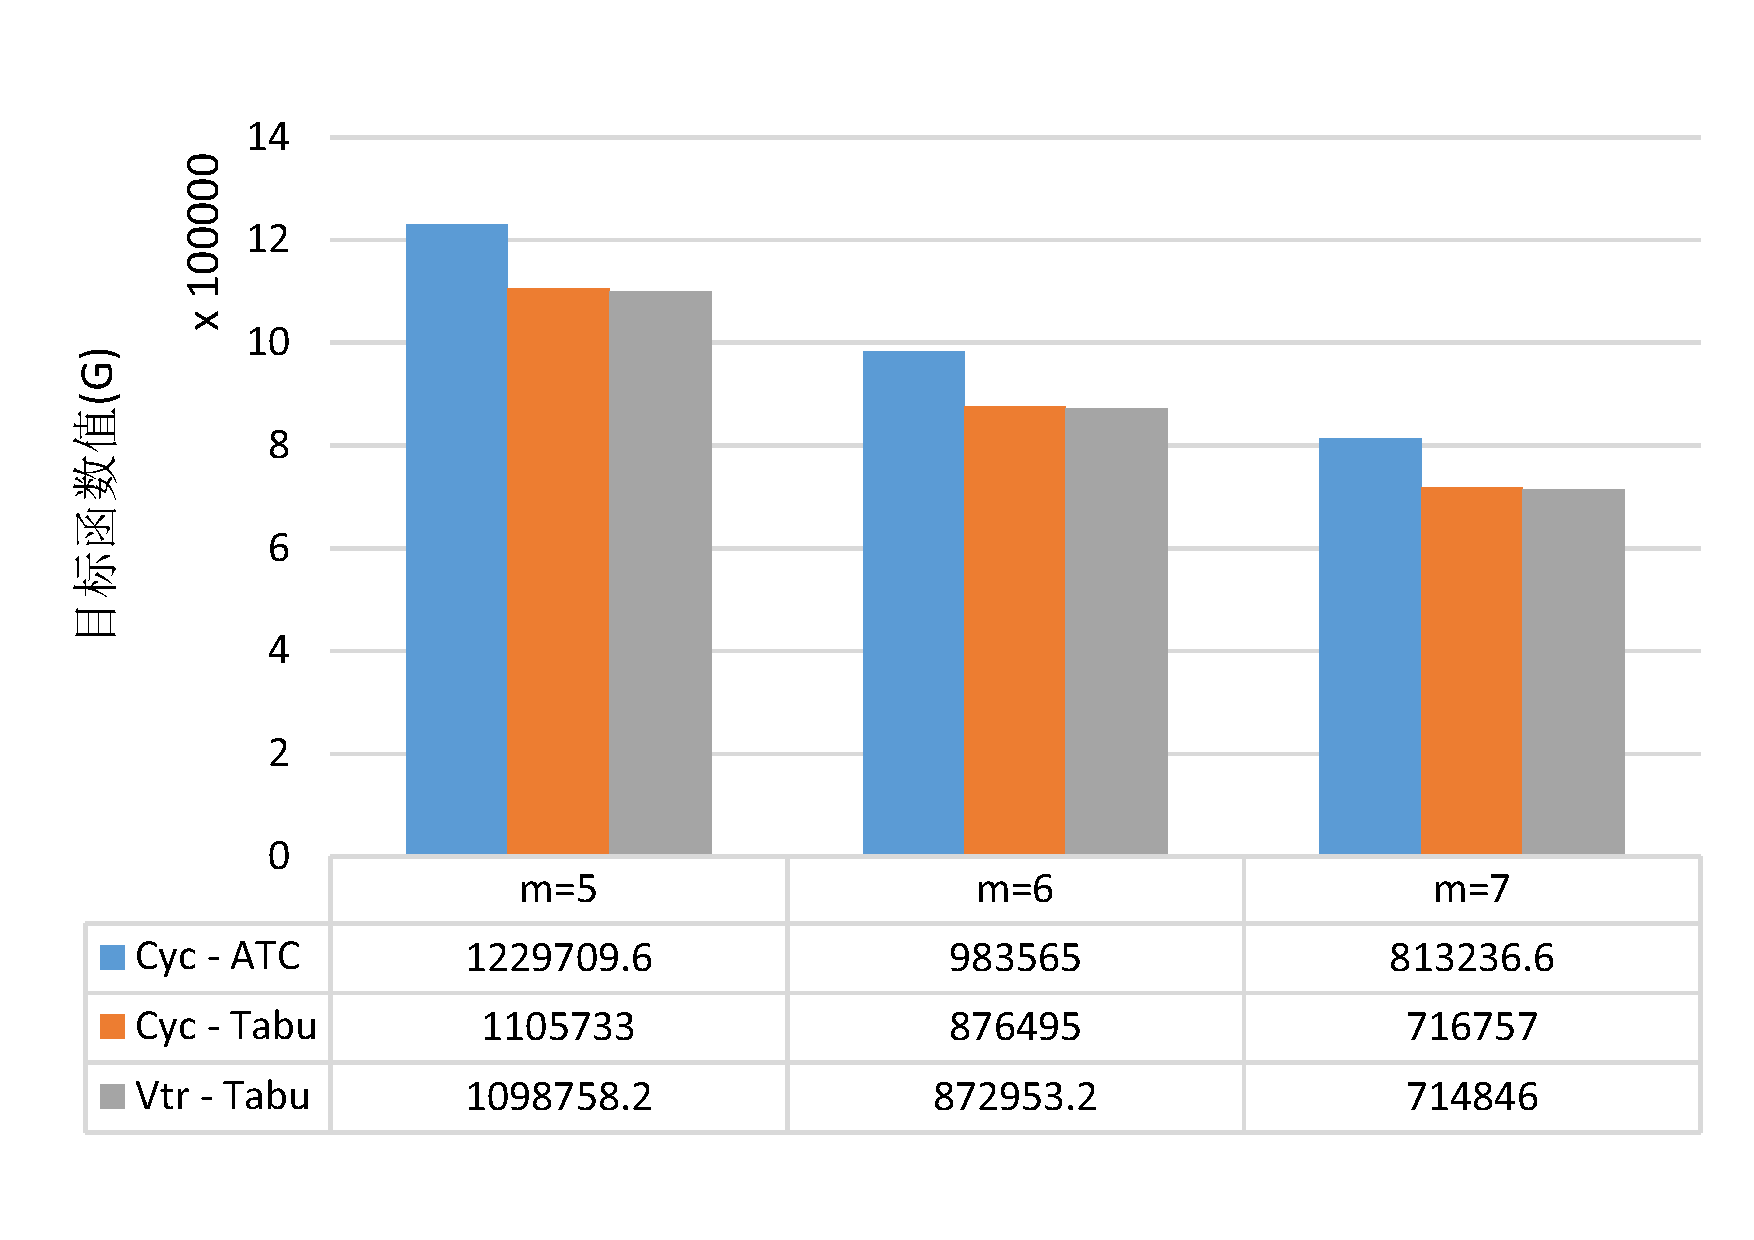
\includegraphics[height = 6cm, angle = -90]{basic_04_300}}
\subfloat[$n = 50$]{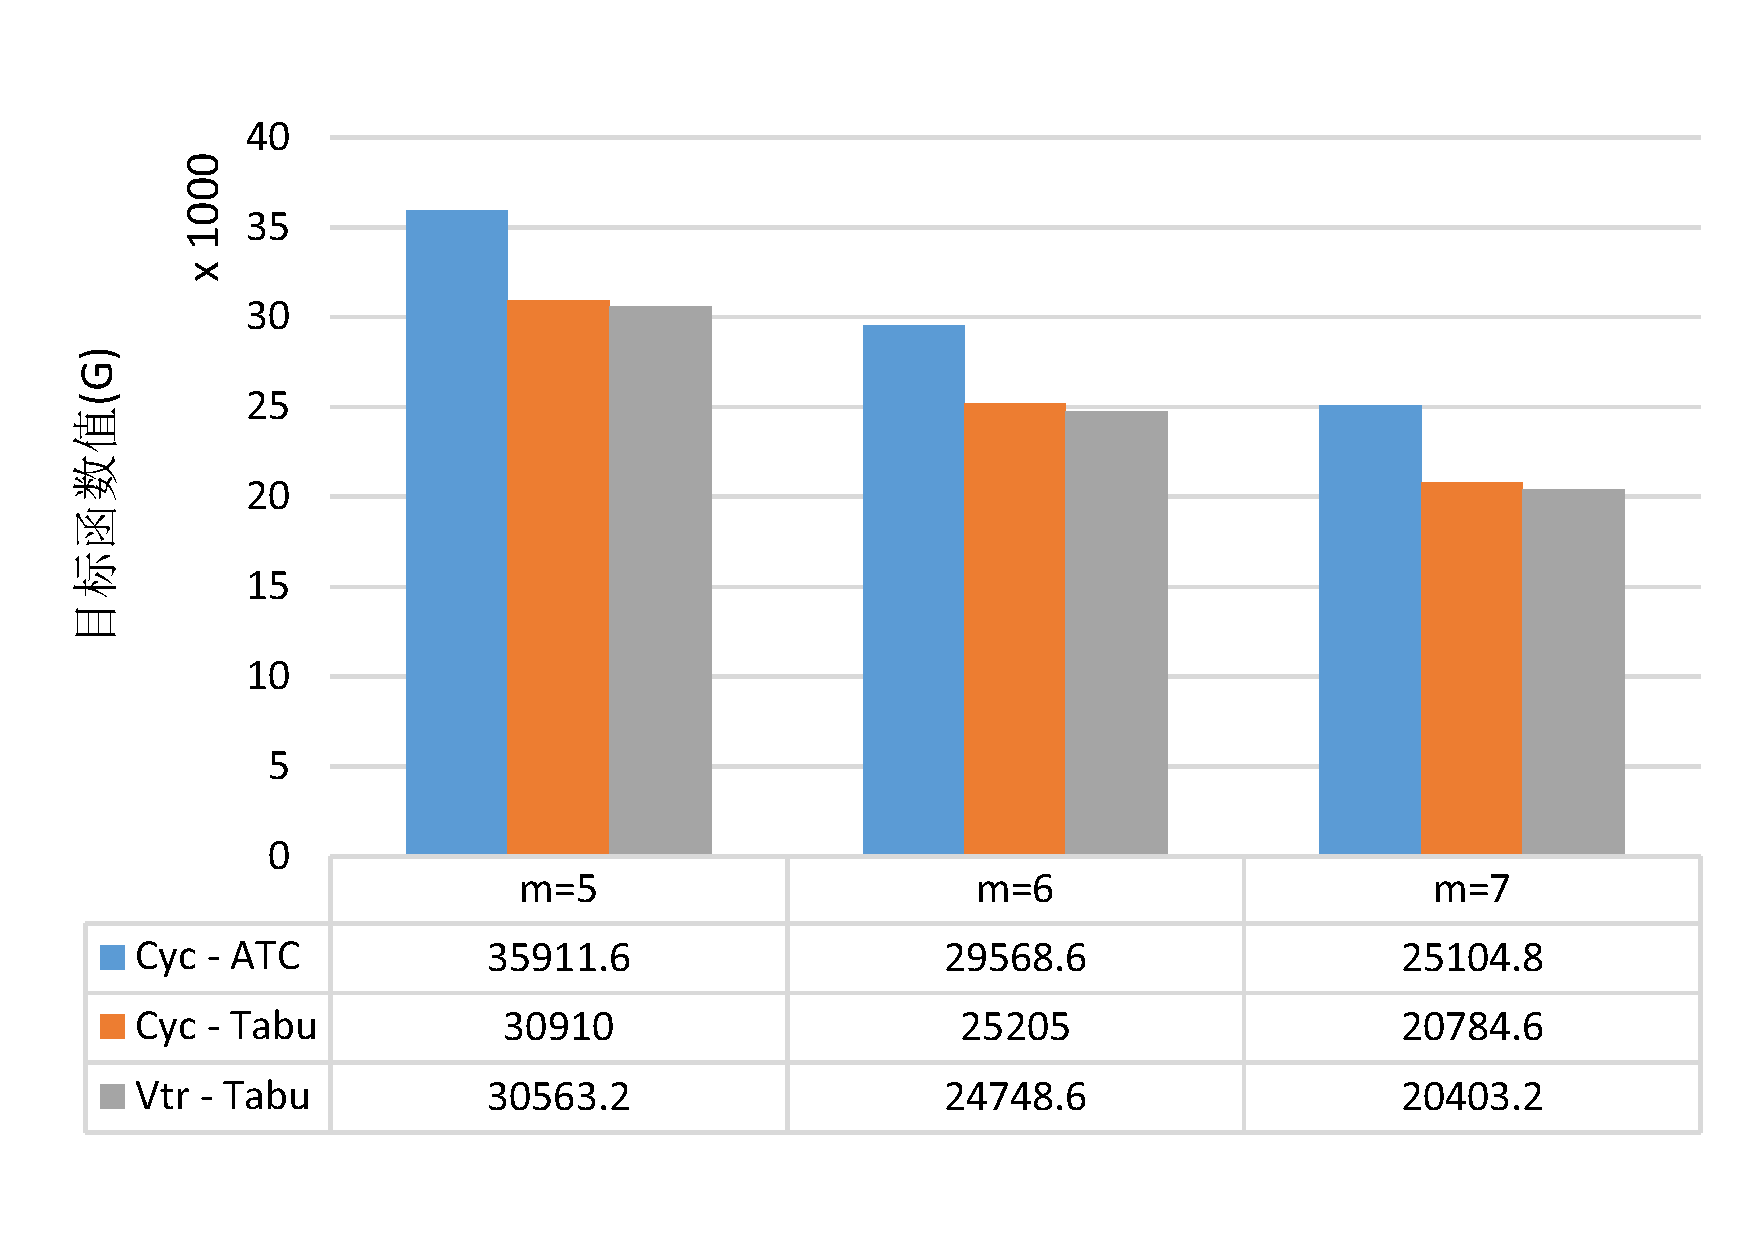
\includegraphics[height = 6cm, angle = -90]{basic_04_50}}
\subfloat[$n = 70$]{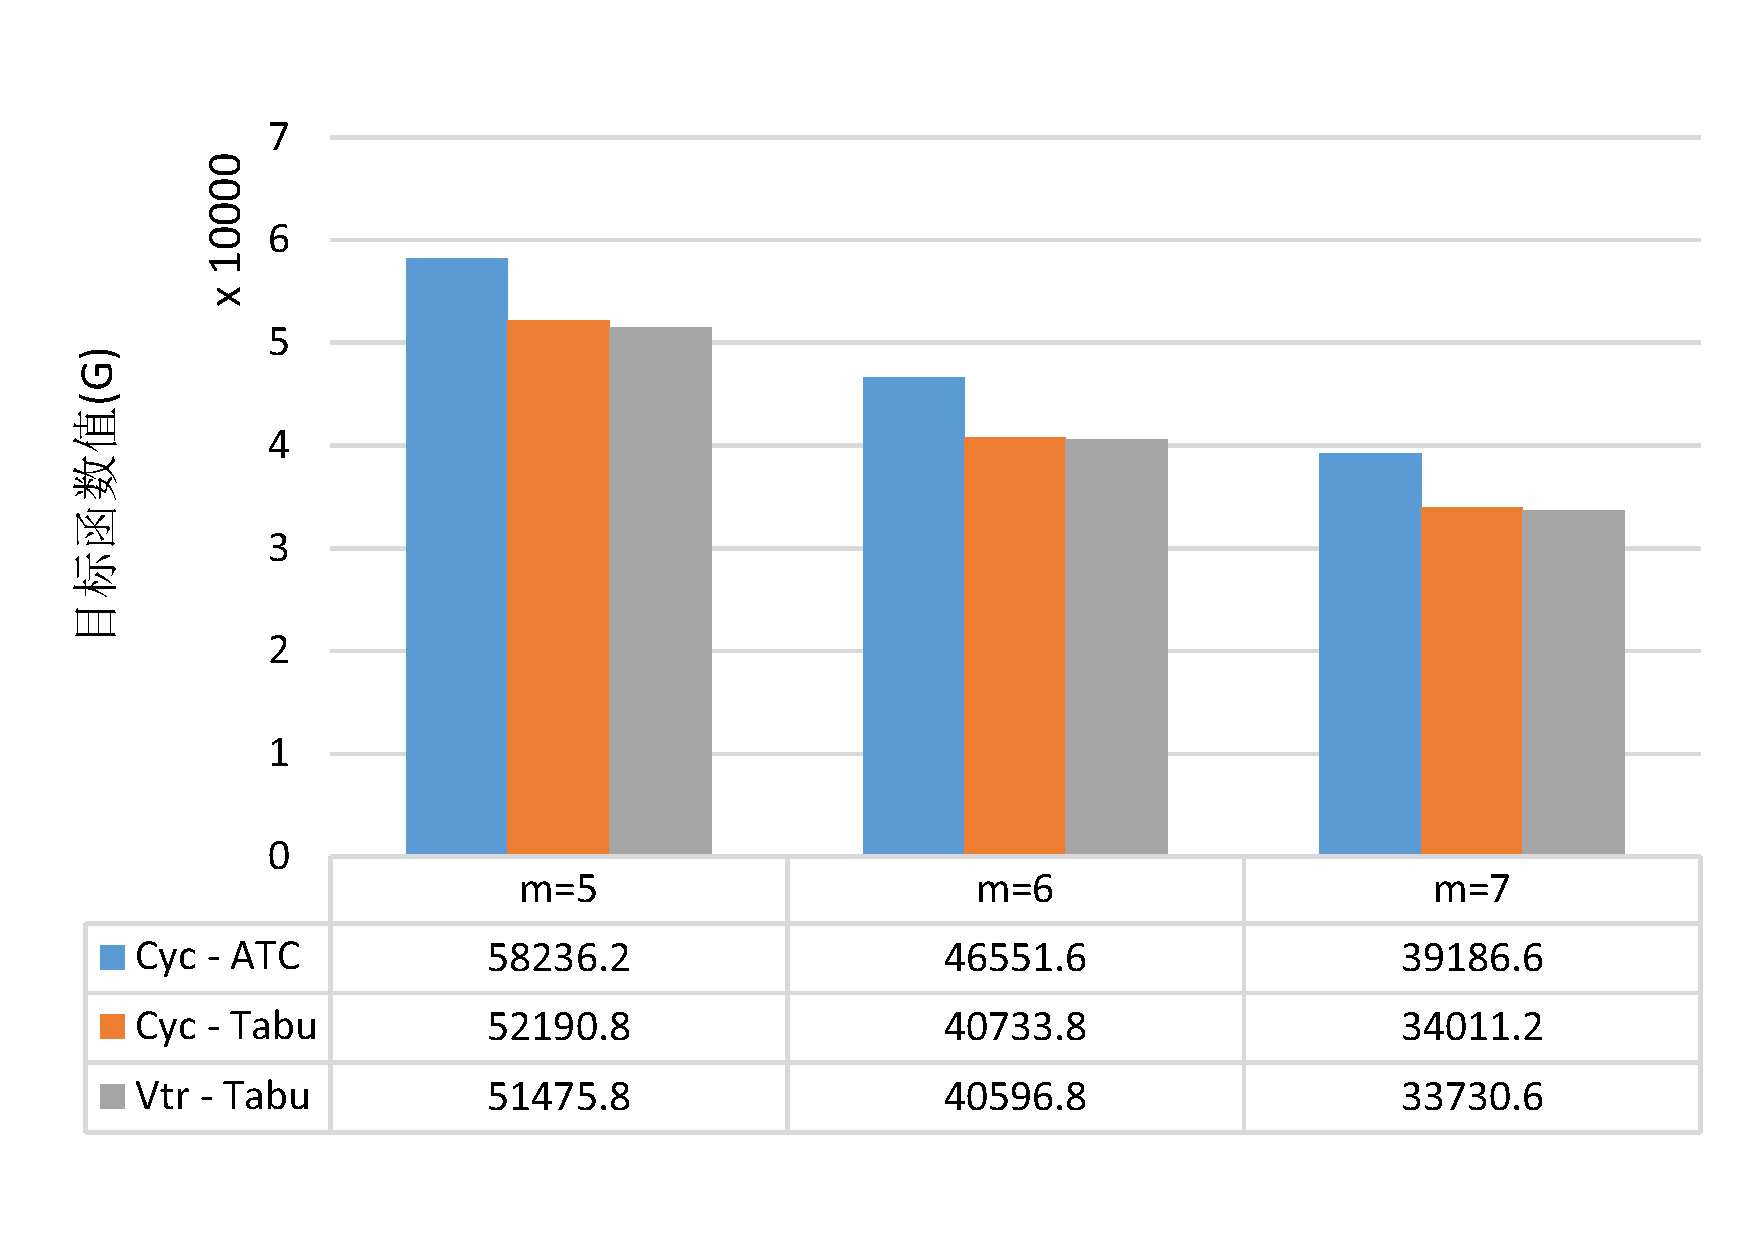
\includegraphics[height = 6cm, angle = -90]{basic_04_70}}\\
\subfloat[$n = 100$]{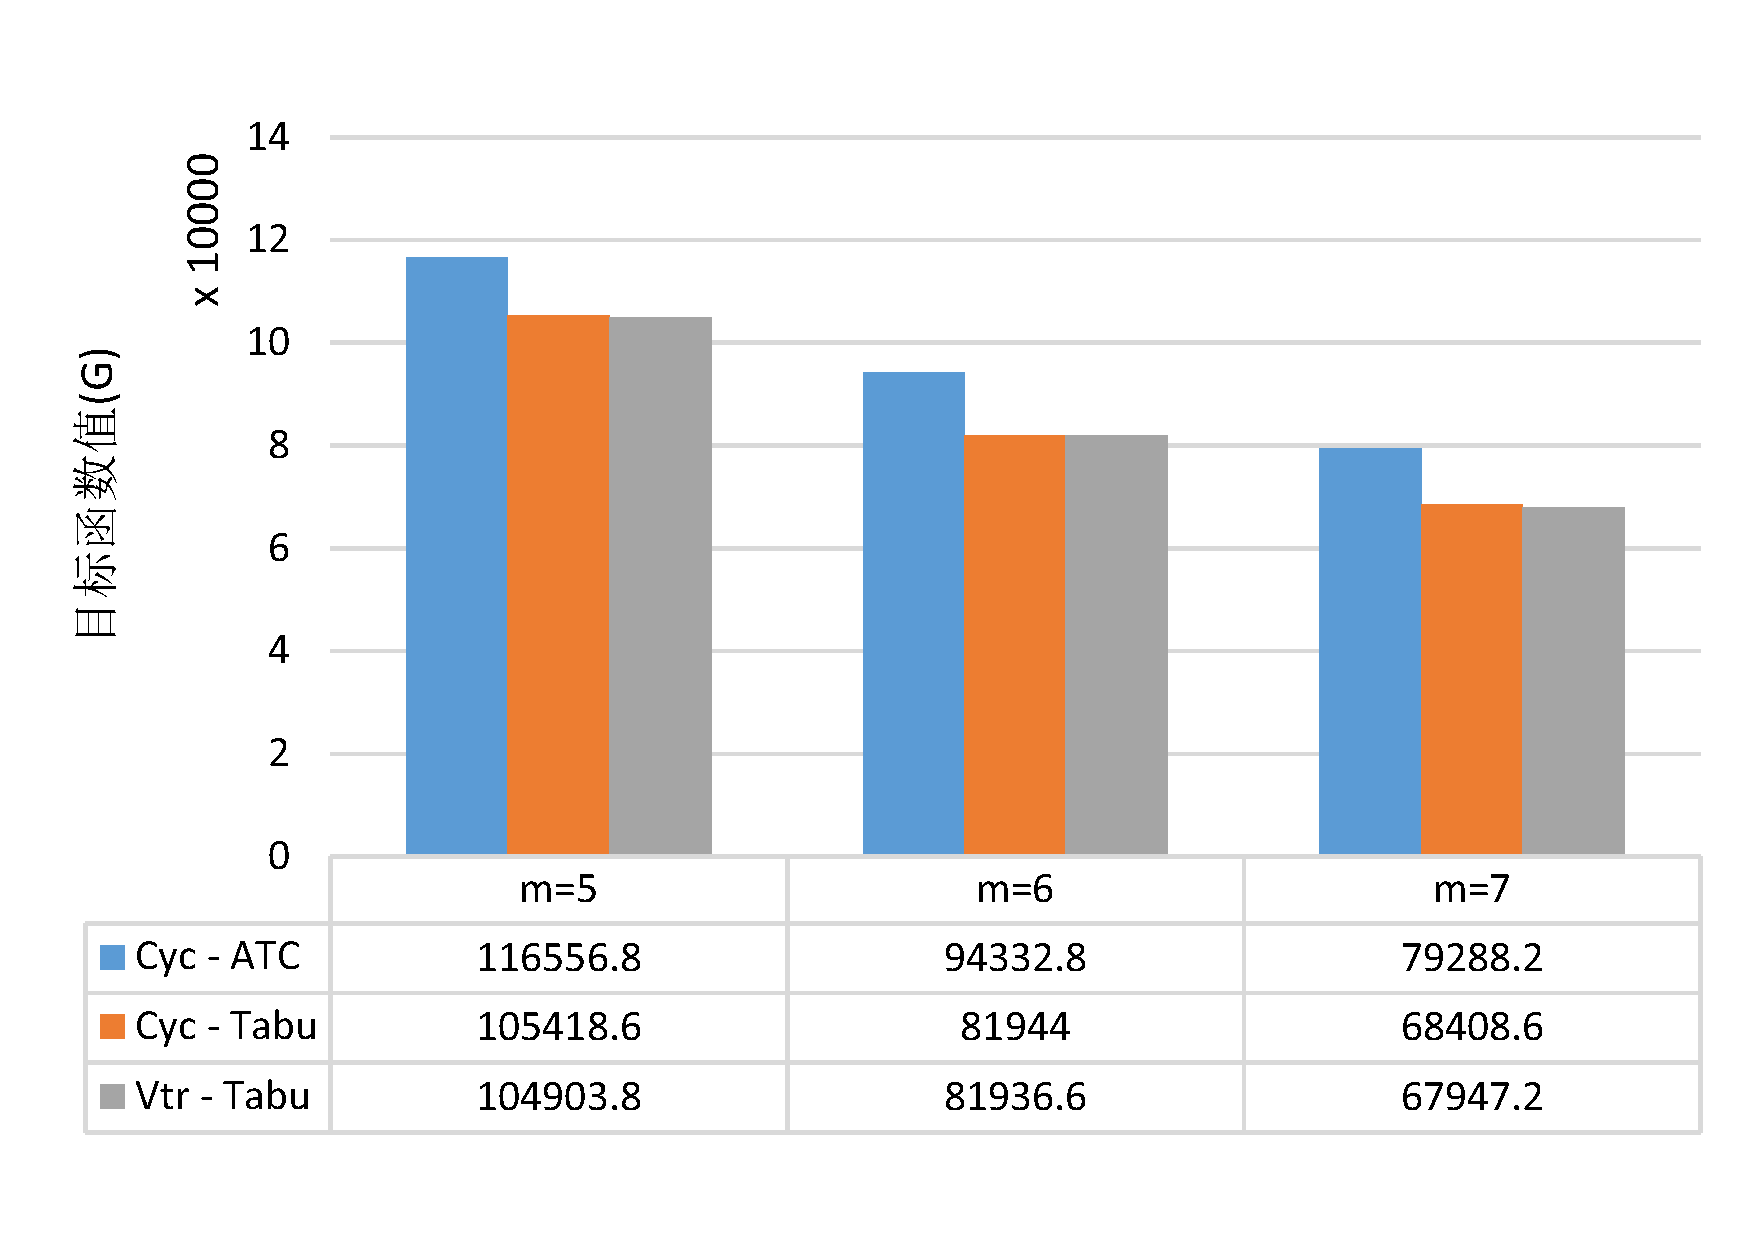
\includegraphics[height = 6cm, angle = -90]{basic_04_100}}
\subfloat[$n = 150$]{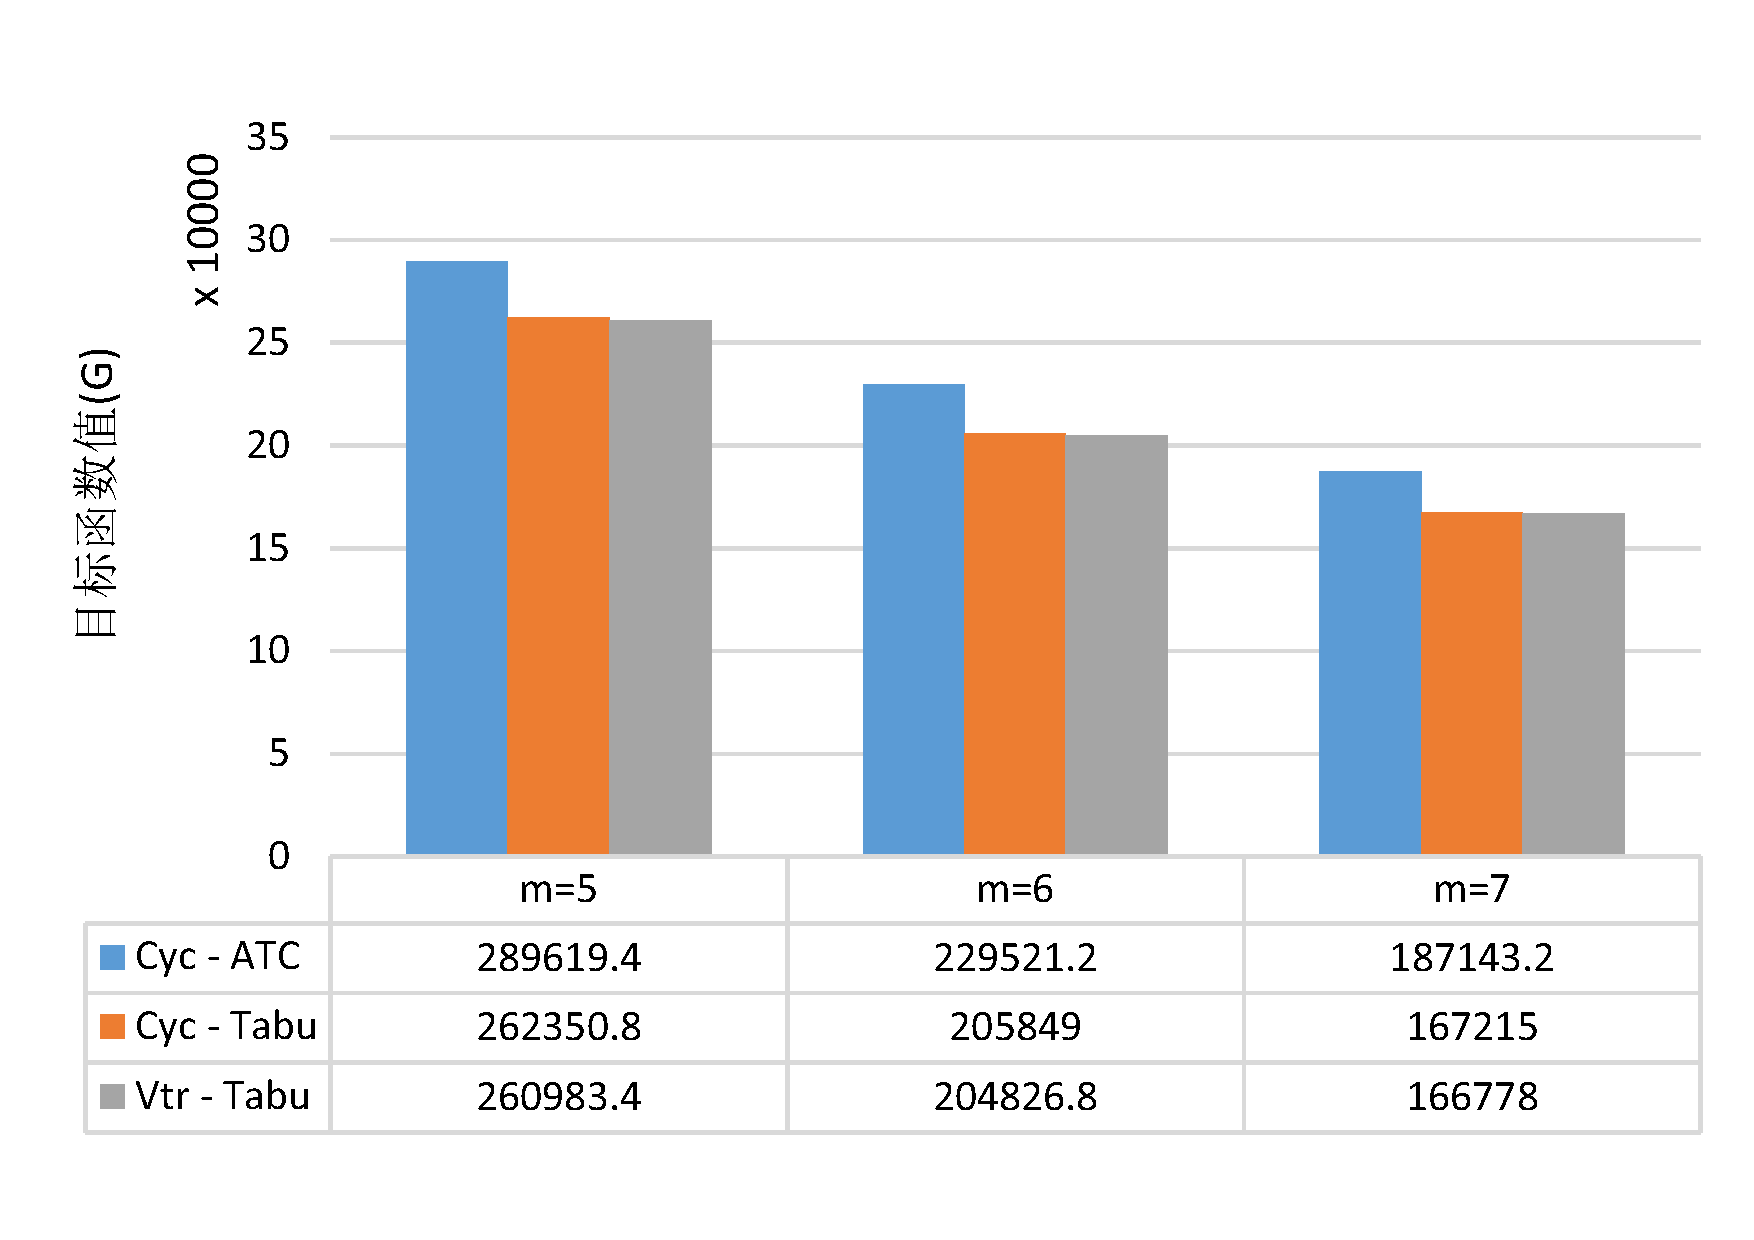
\includegraphics[height = 6cm, angle = -90]{basic_04_150}}
\subfloat[$n = 200$]{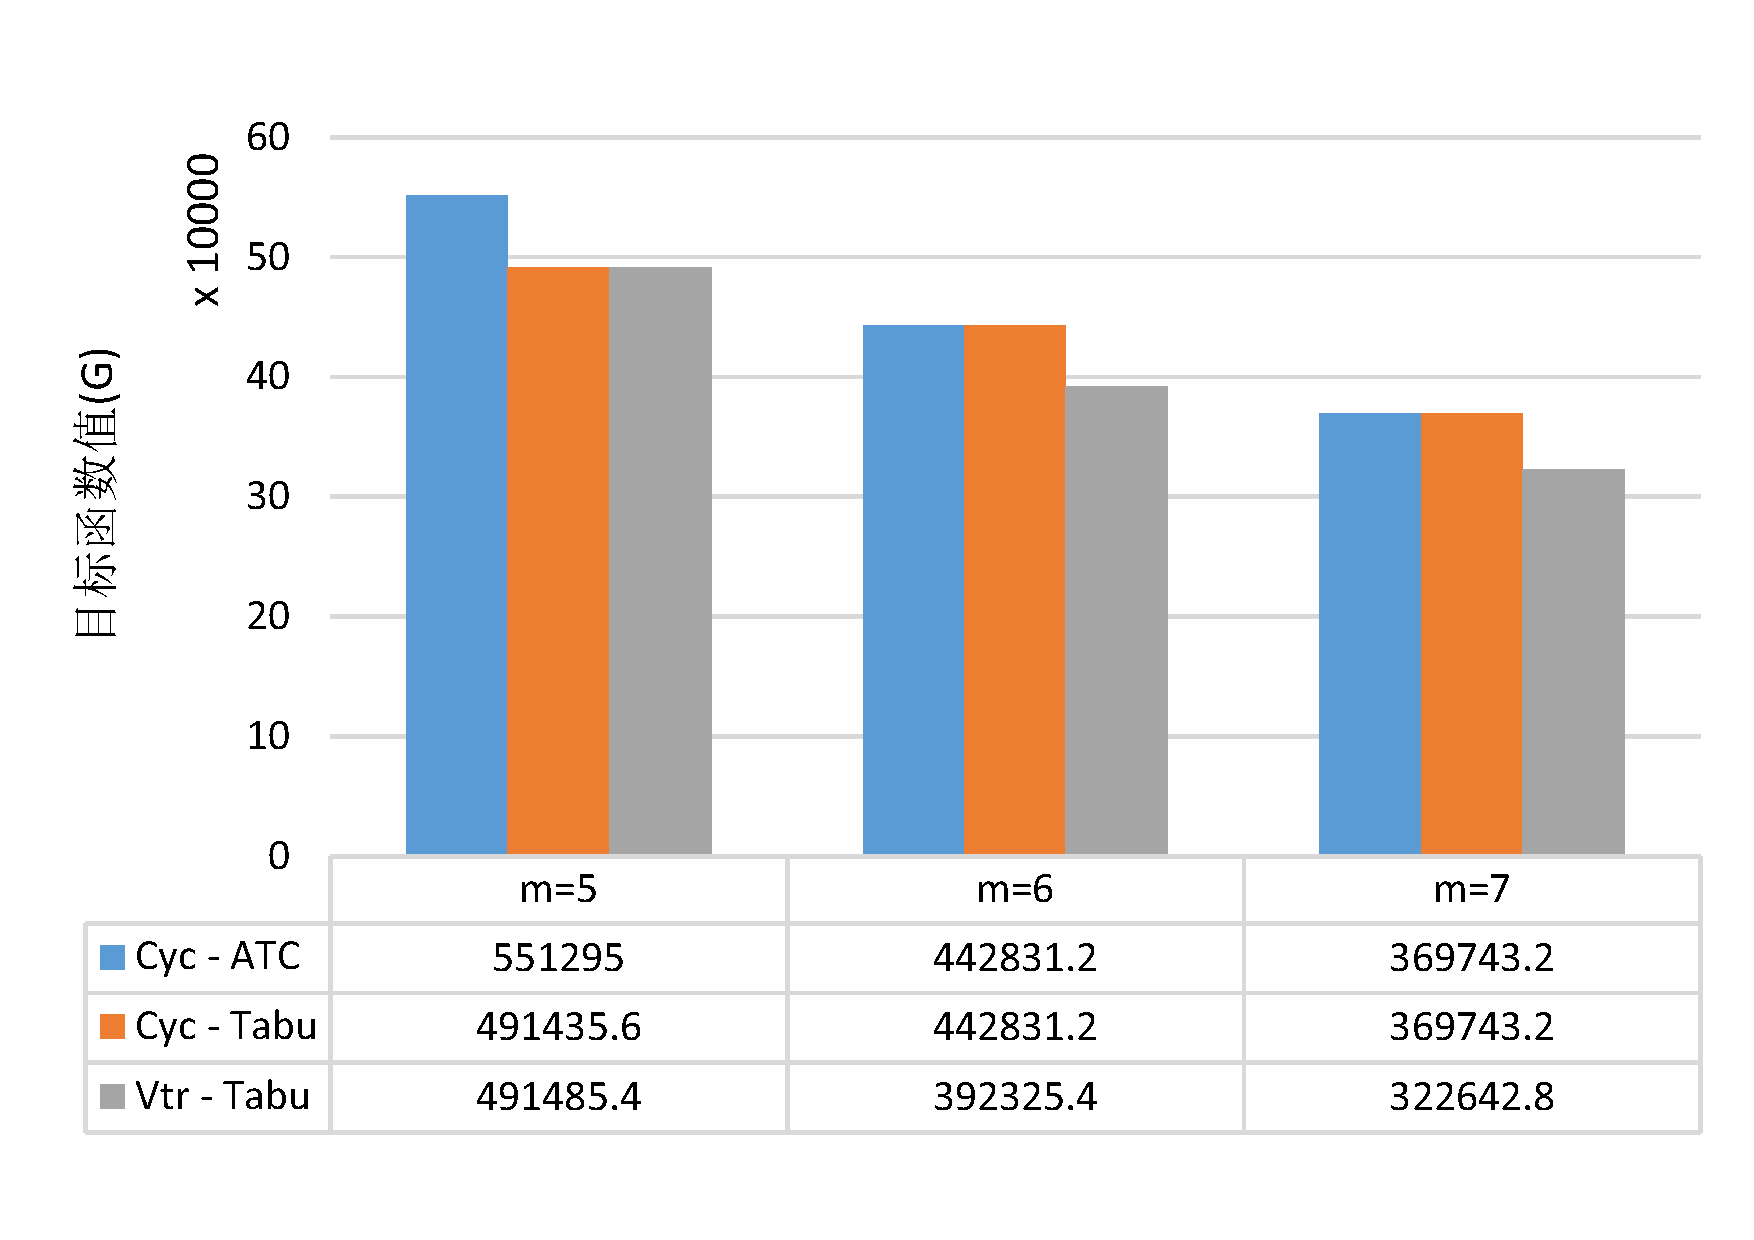
\includegraphics[height = 6cm, angle = -90]{basic_04_200}}
\subfloat[$n = 300$]{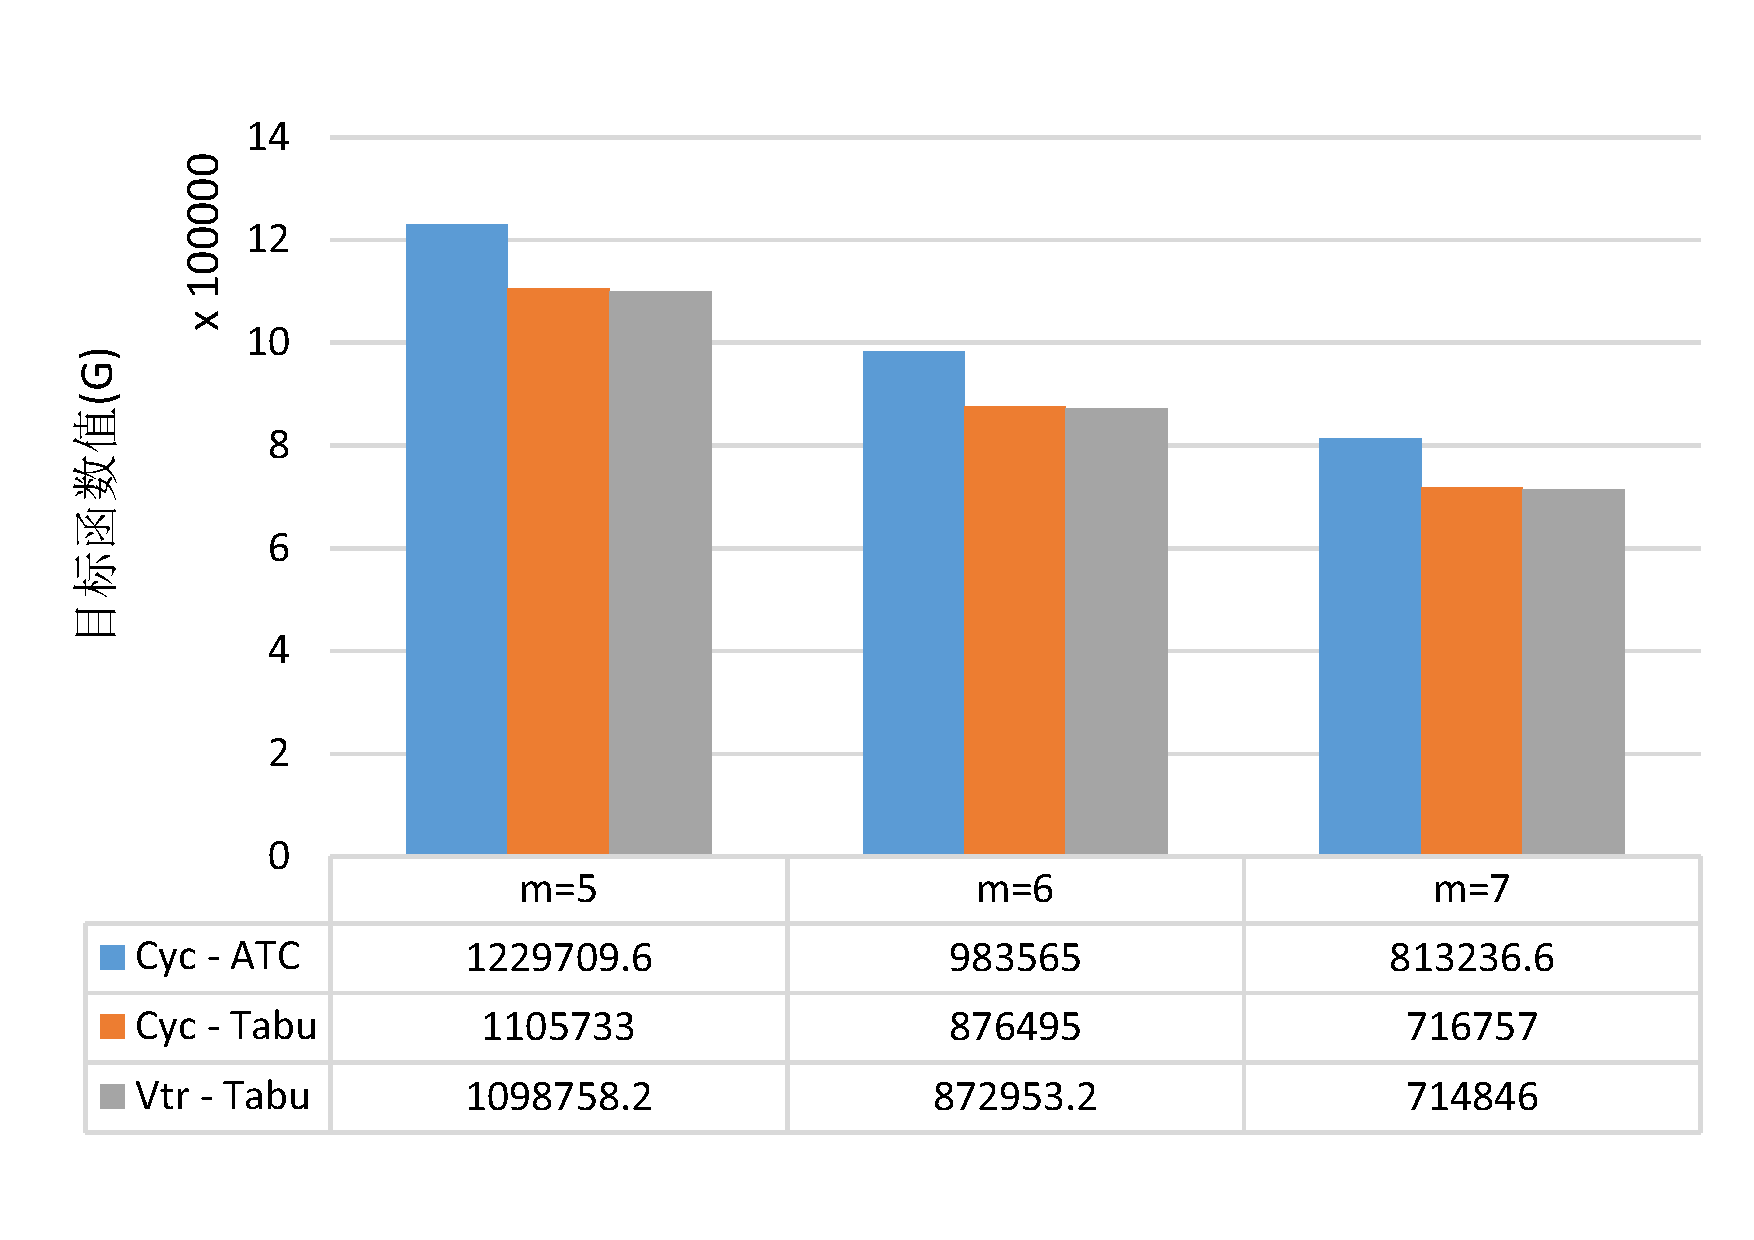
\includegraphics[height = 6cm, angle = -90]{basic_04_300}}\\
\subfloat[$n = 500$]{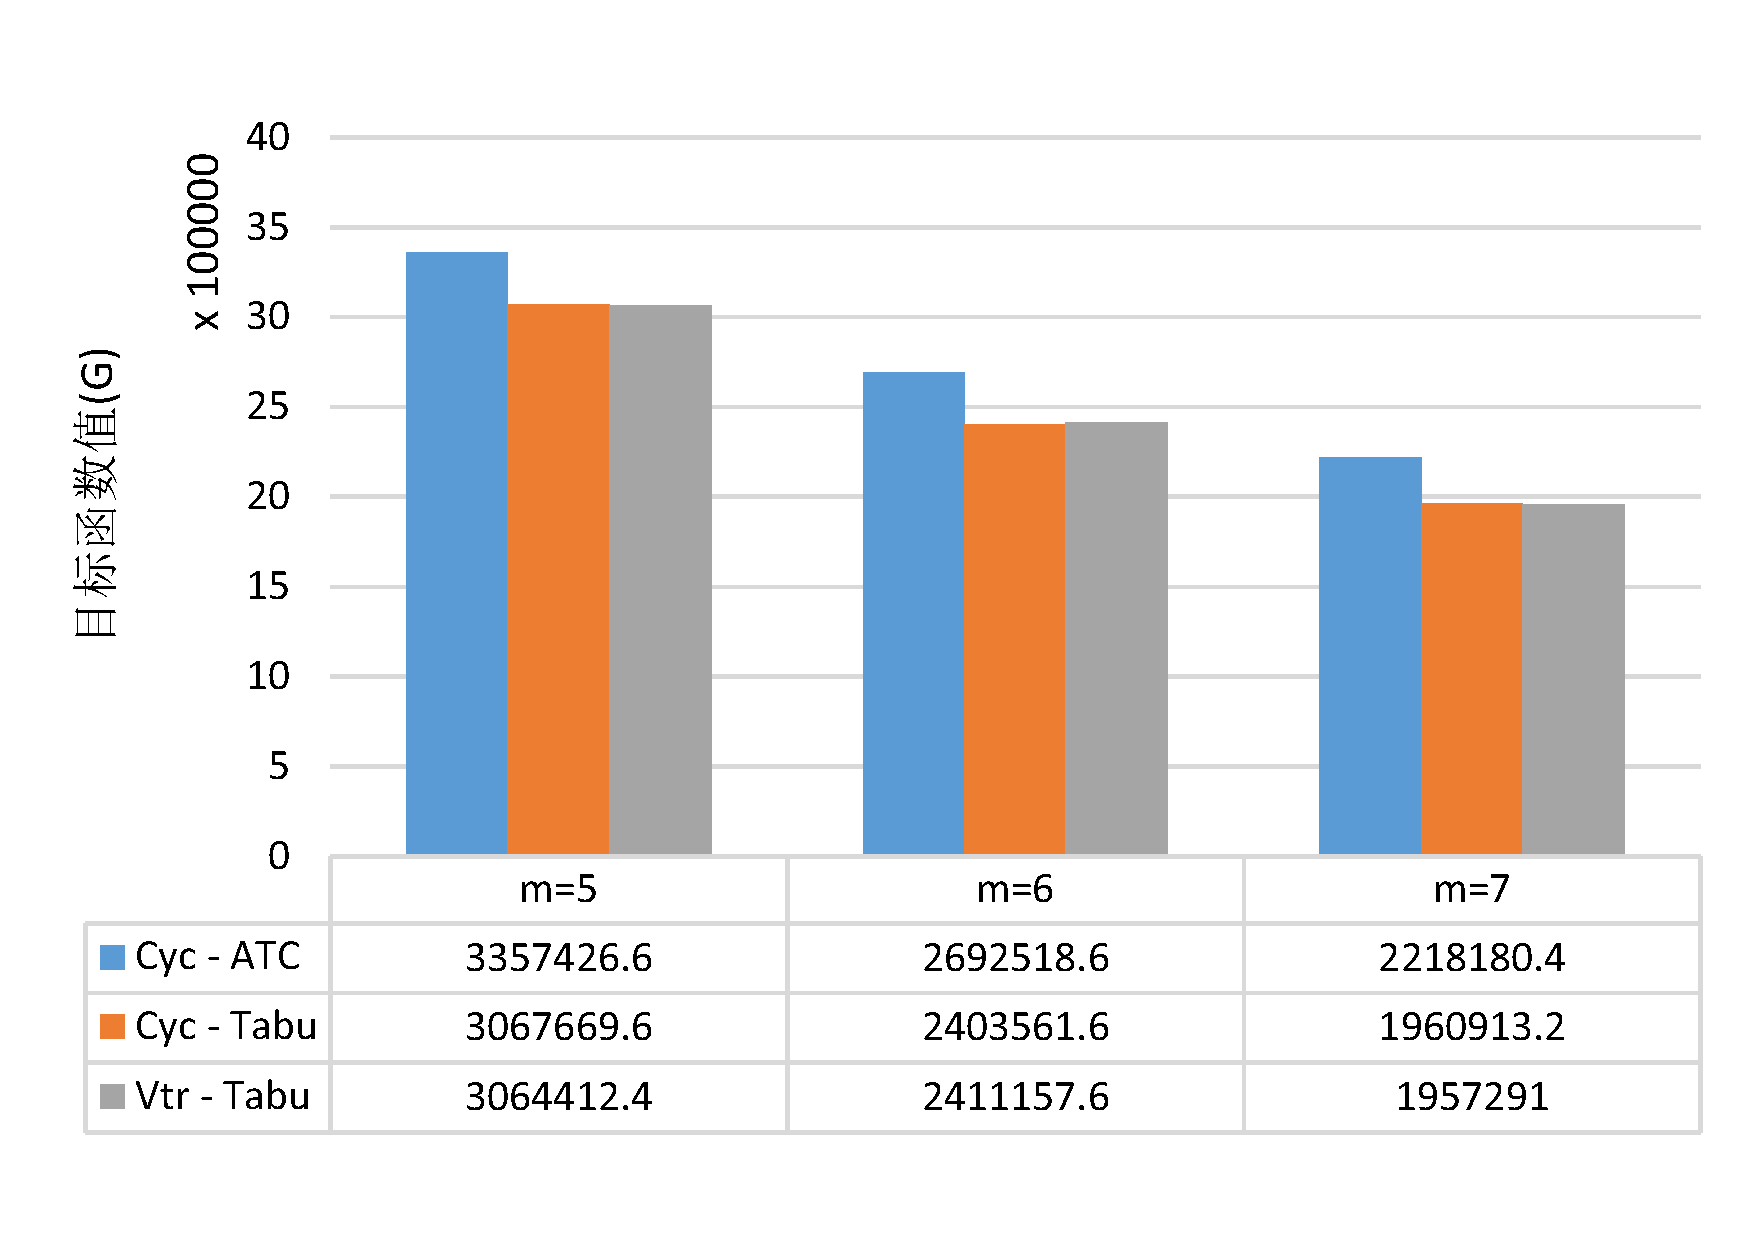
\includegraphics[height = 6cm, angle = -90]{basic_04_500}}
\subfloat[$n = 750$]{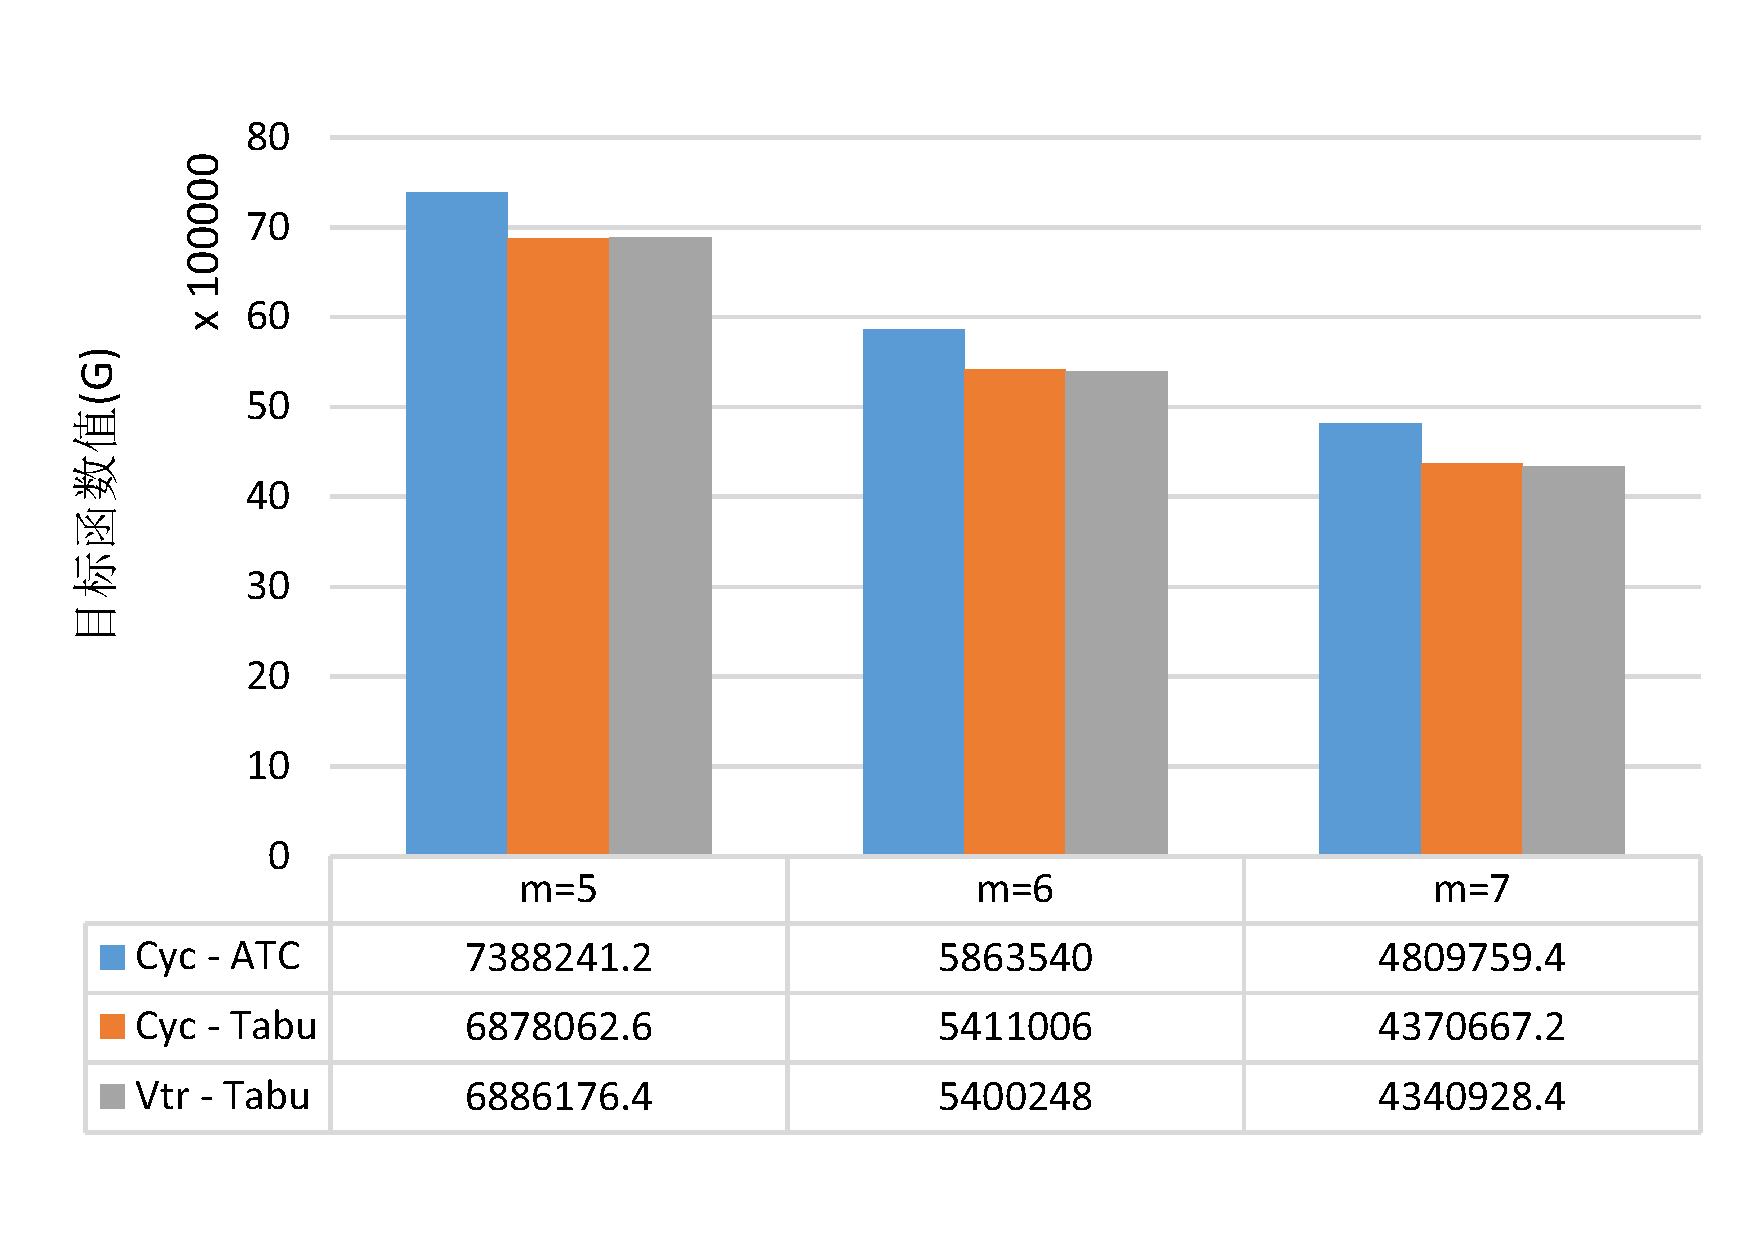
\includegraphics[height = 6cm, angle = -90]{basic_04_750}}
\subfloat[$n = 1000$]{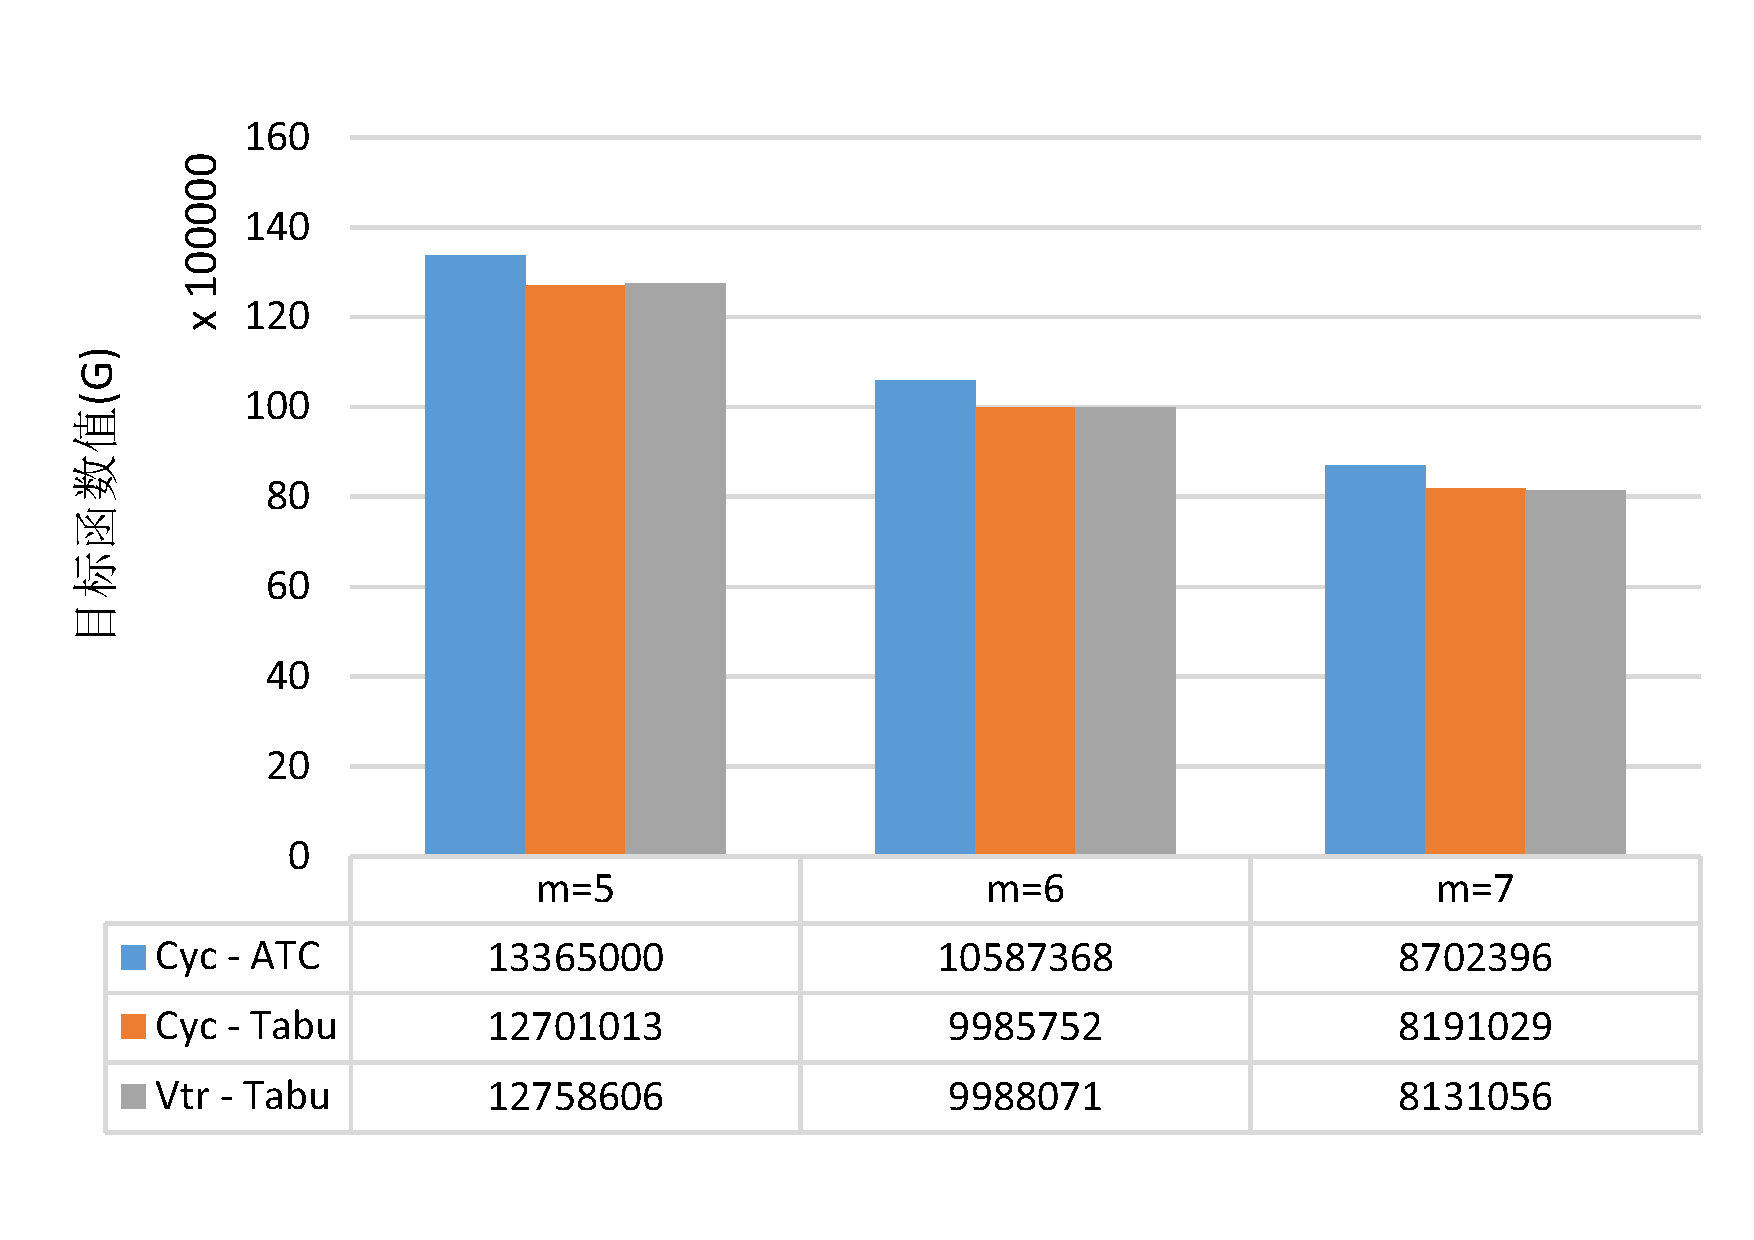
\includegraphics[height = 6cm, angle = -90]{basic_04_1000}}
\caption{\label{fig:result1}模型$1$的Cyc -- ATC、Cyc -- Tabu、Vtr -- Tabu 算法求解目标函数值比较$(\lambda_1 = 0.4)$}
\end{sidewaysfigure}

\begin{sidewaysfigure}
\centering
\subfloat[$n = 20$]{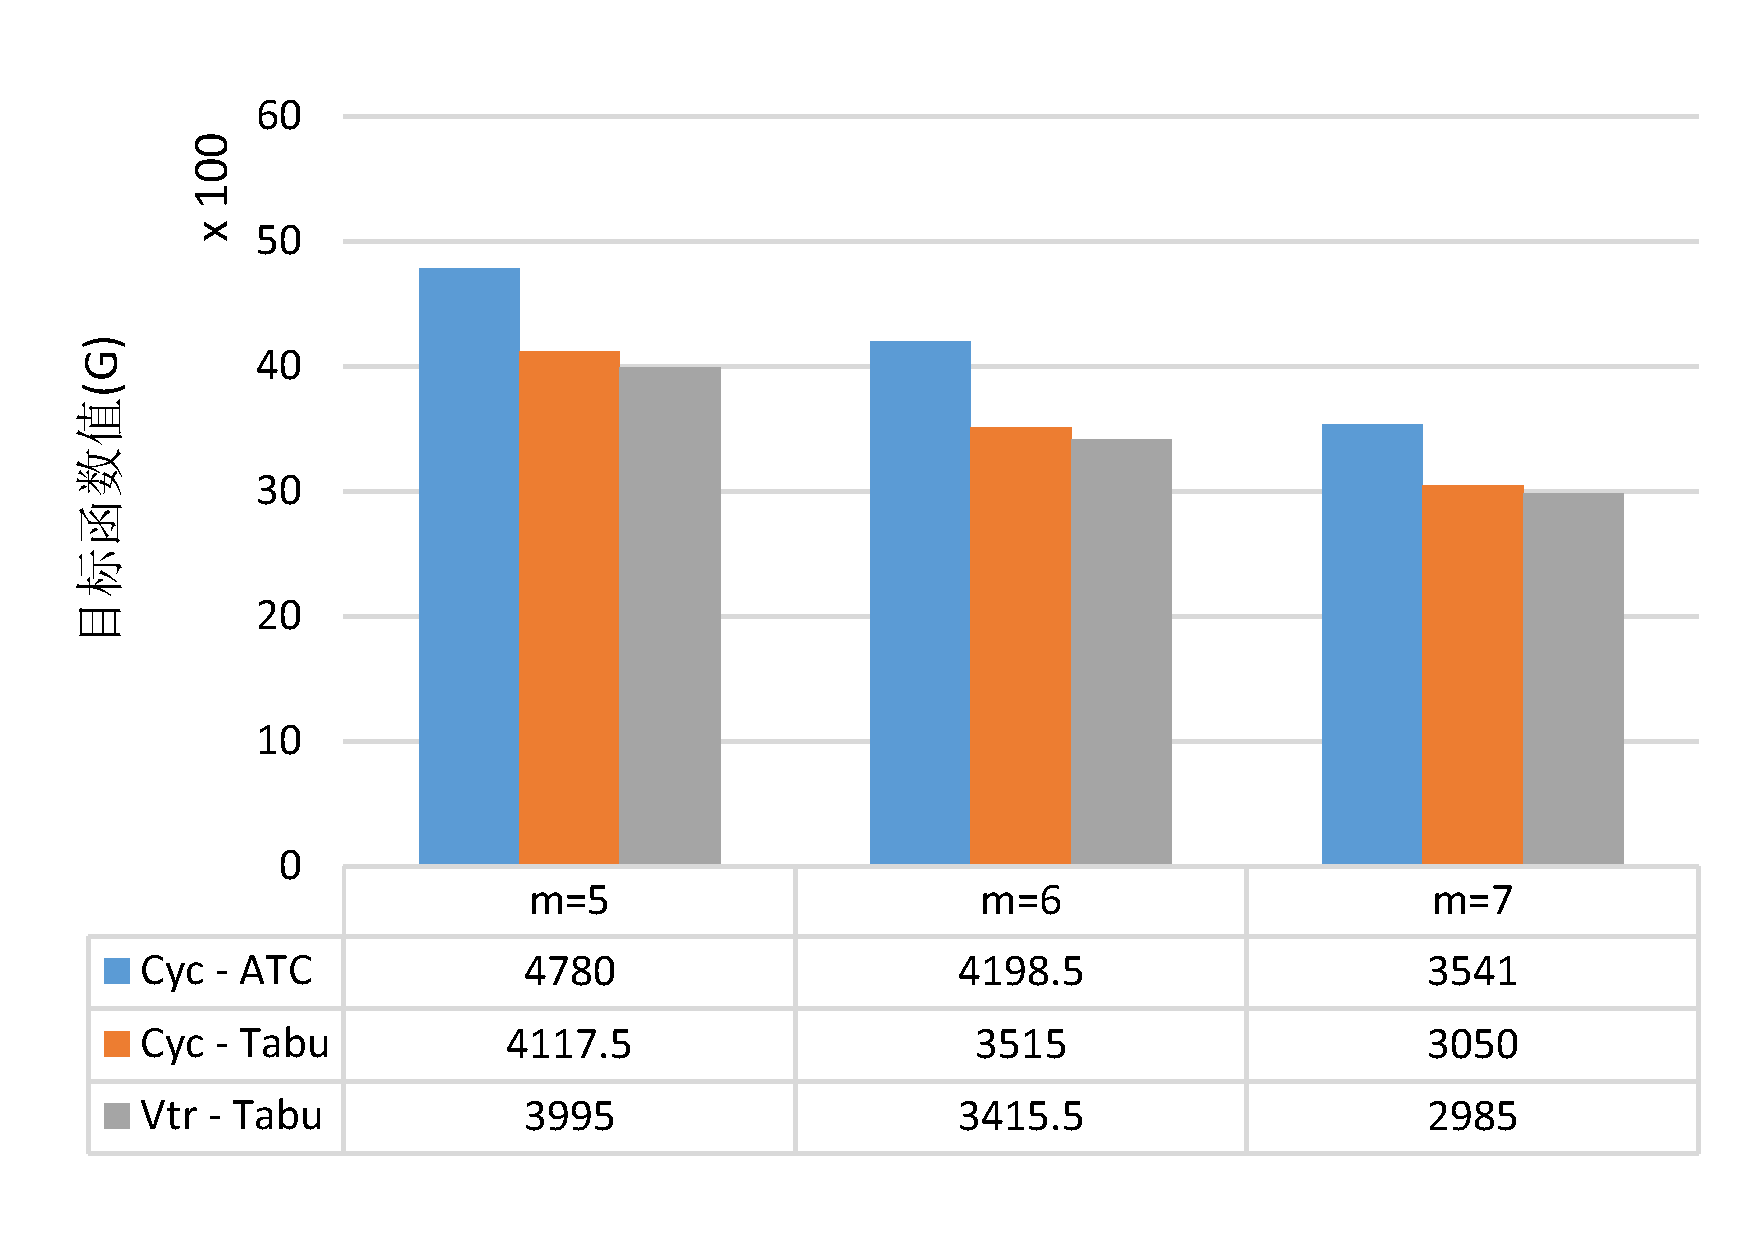
\includegraphics[height = 6cm, angle = -90]{basic_05_20}}
\subfloat[$n = 30$]{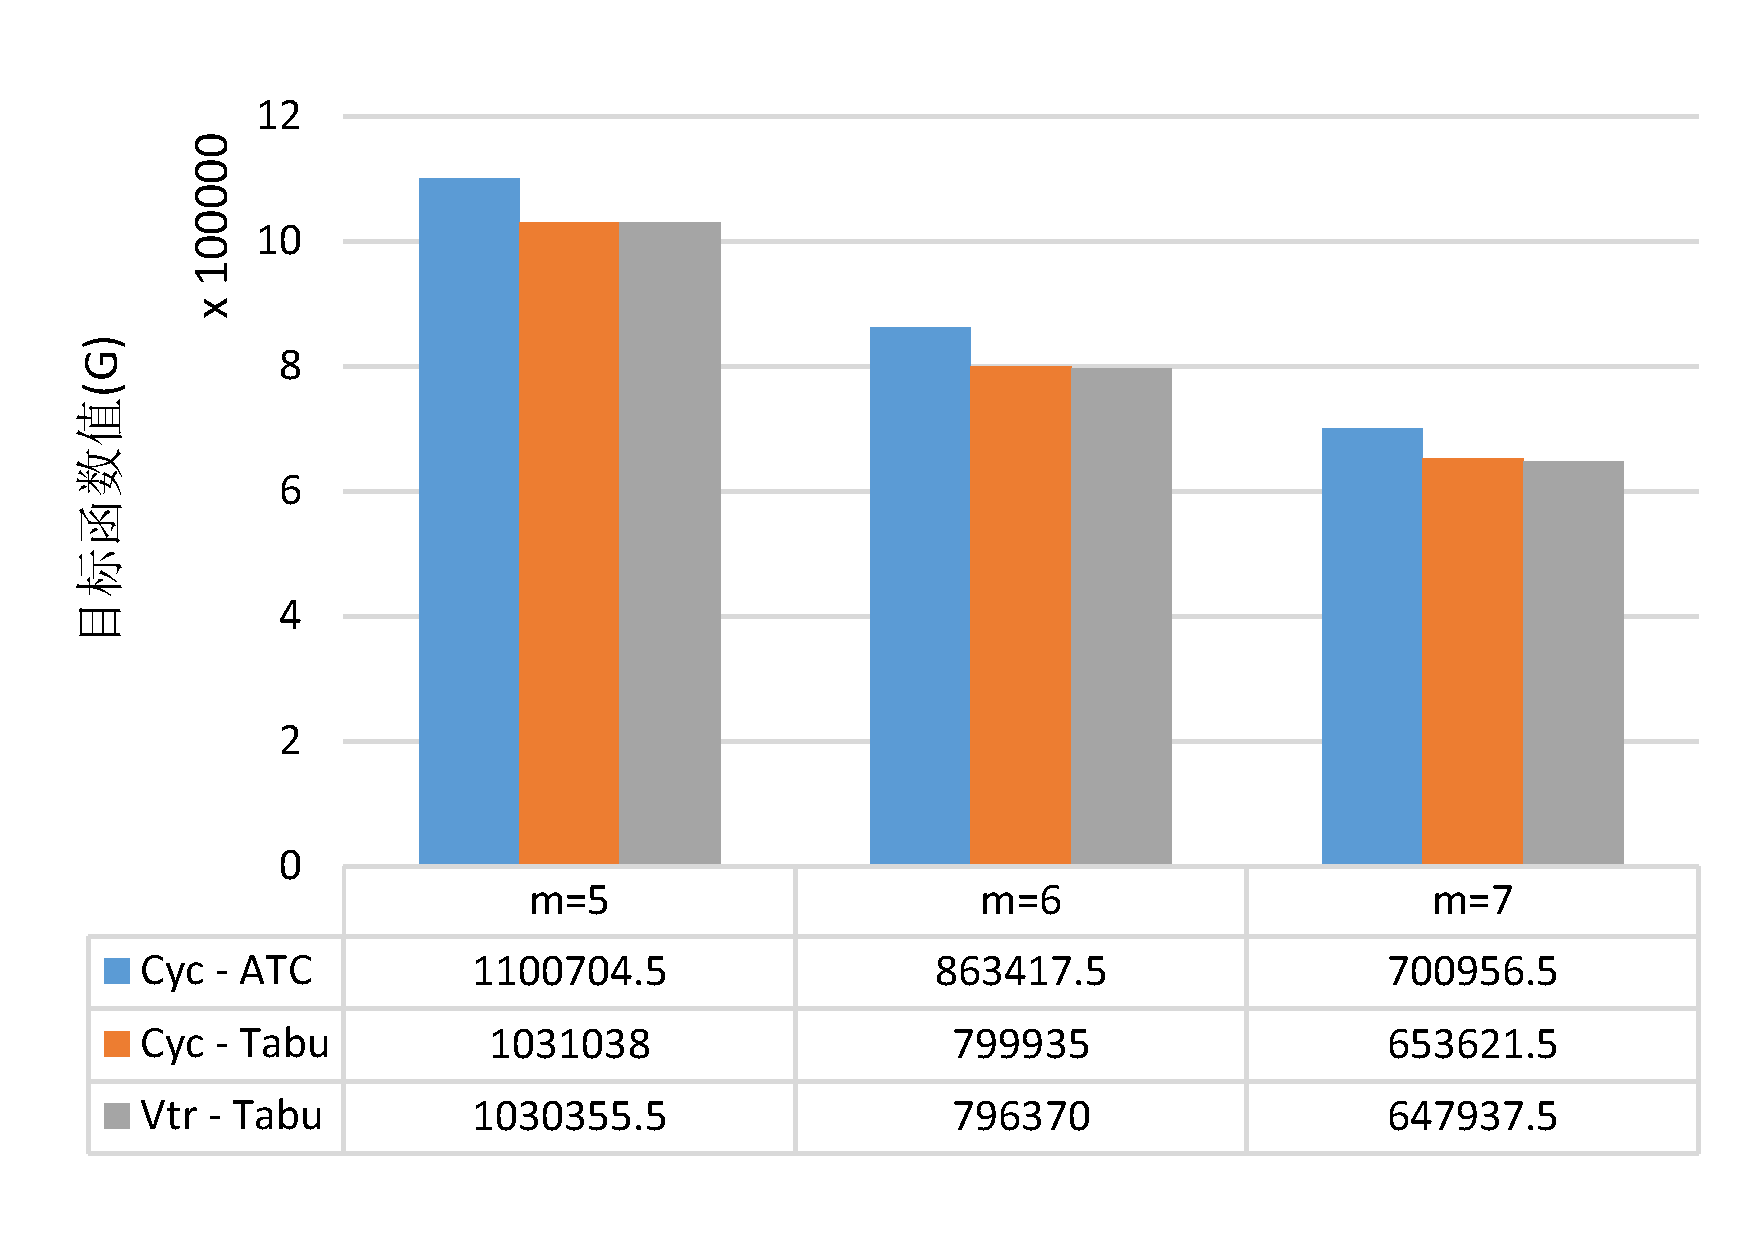
\includegraphics[height = 6cm, angle = -90]{basic_05_300}}
\subfloat[$n = 50$]{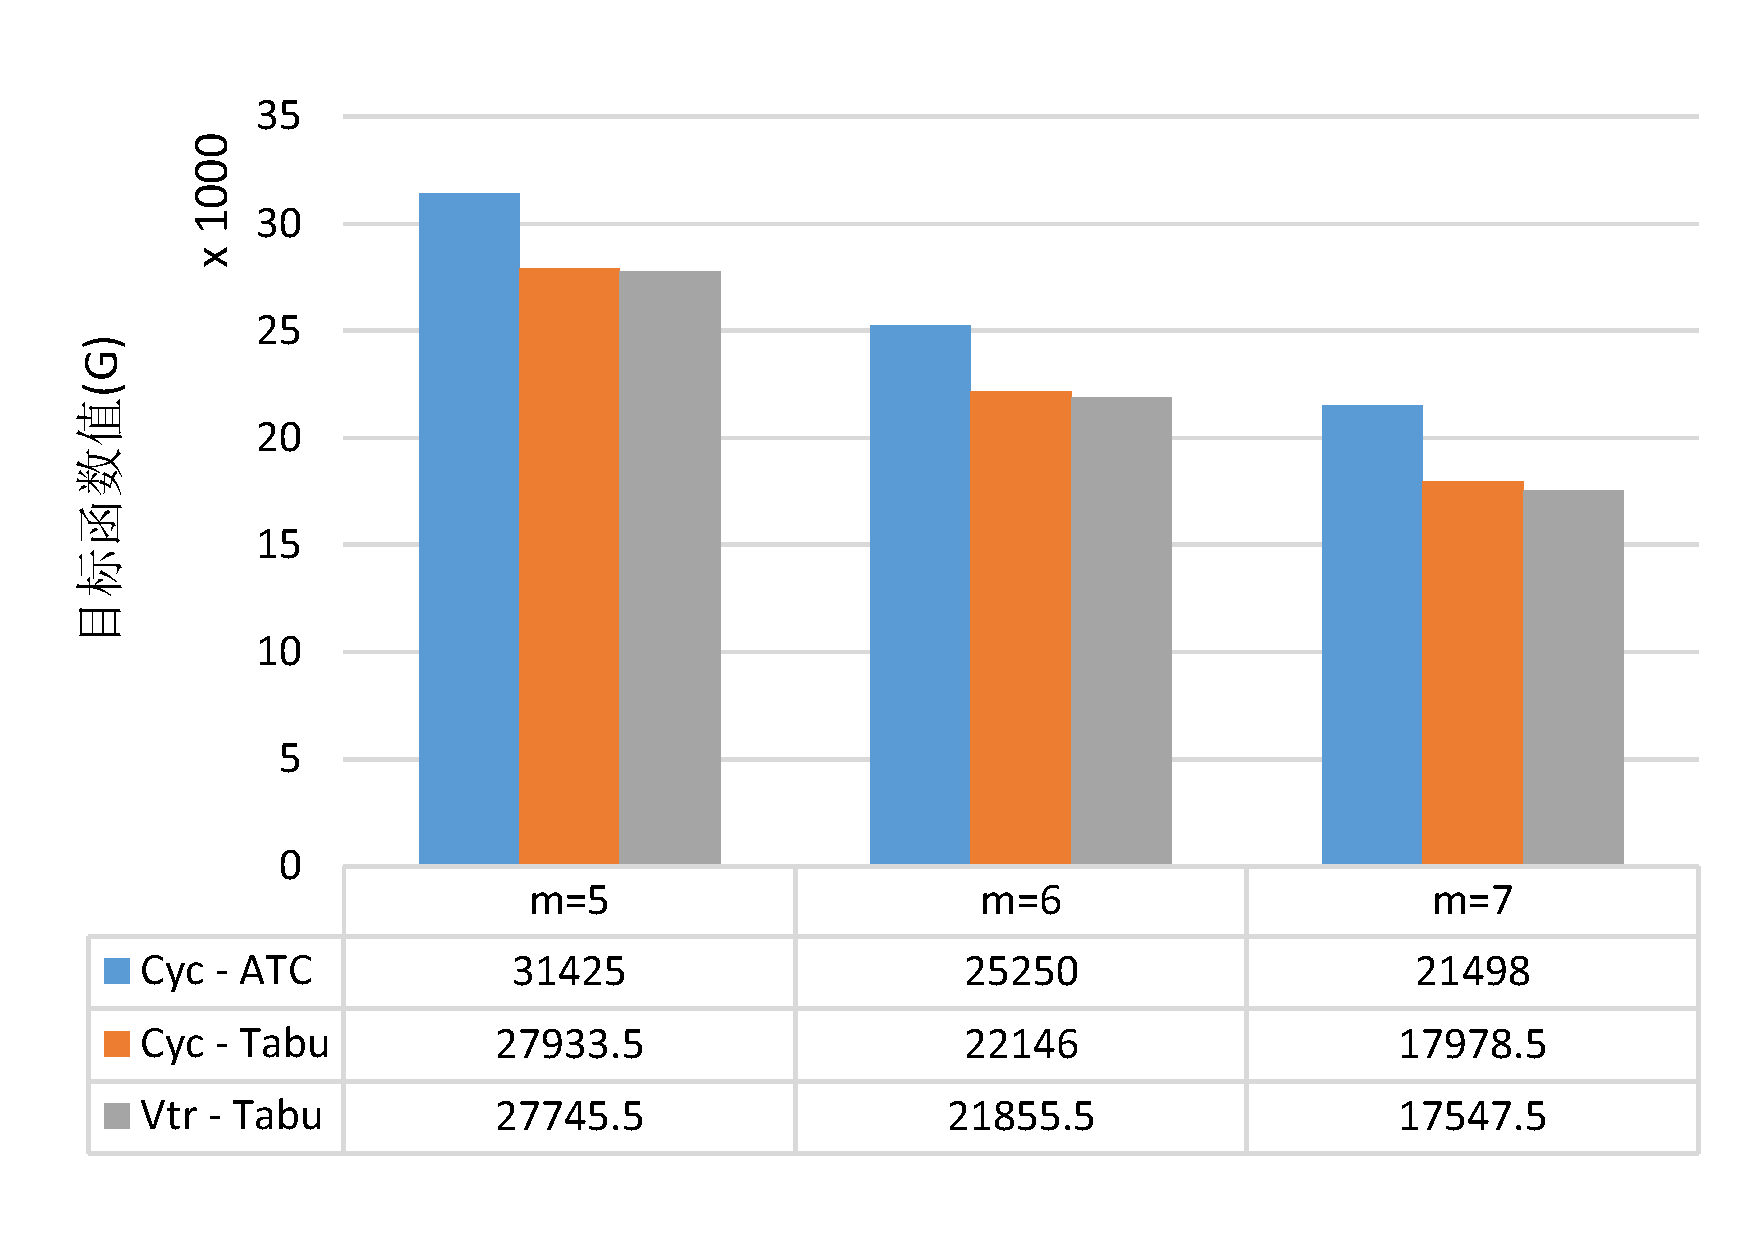
\includegraphics[height = 6cm, angle = -90]{basic_05_50}}
\subfloat[$n = 70$]{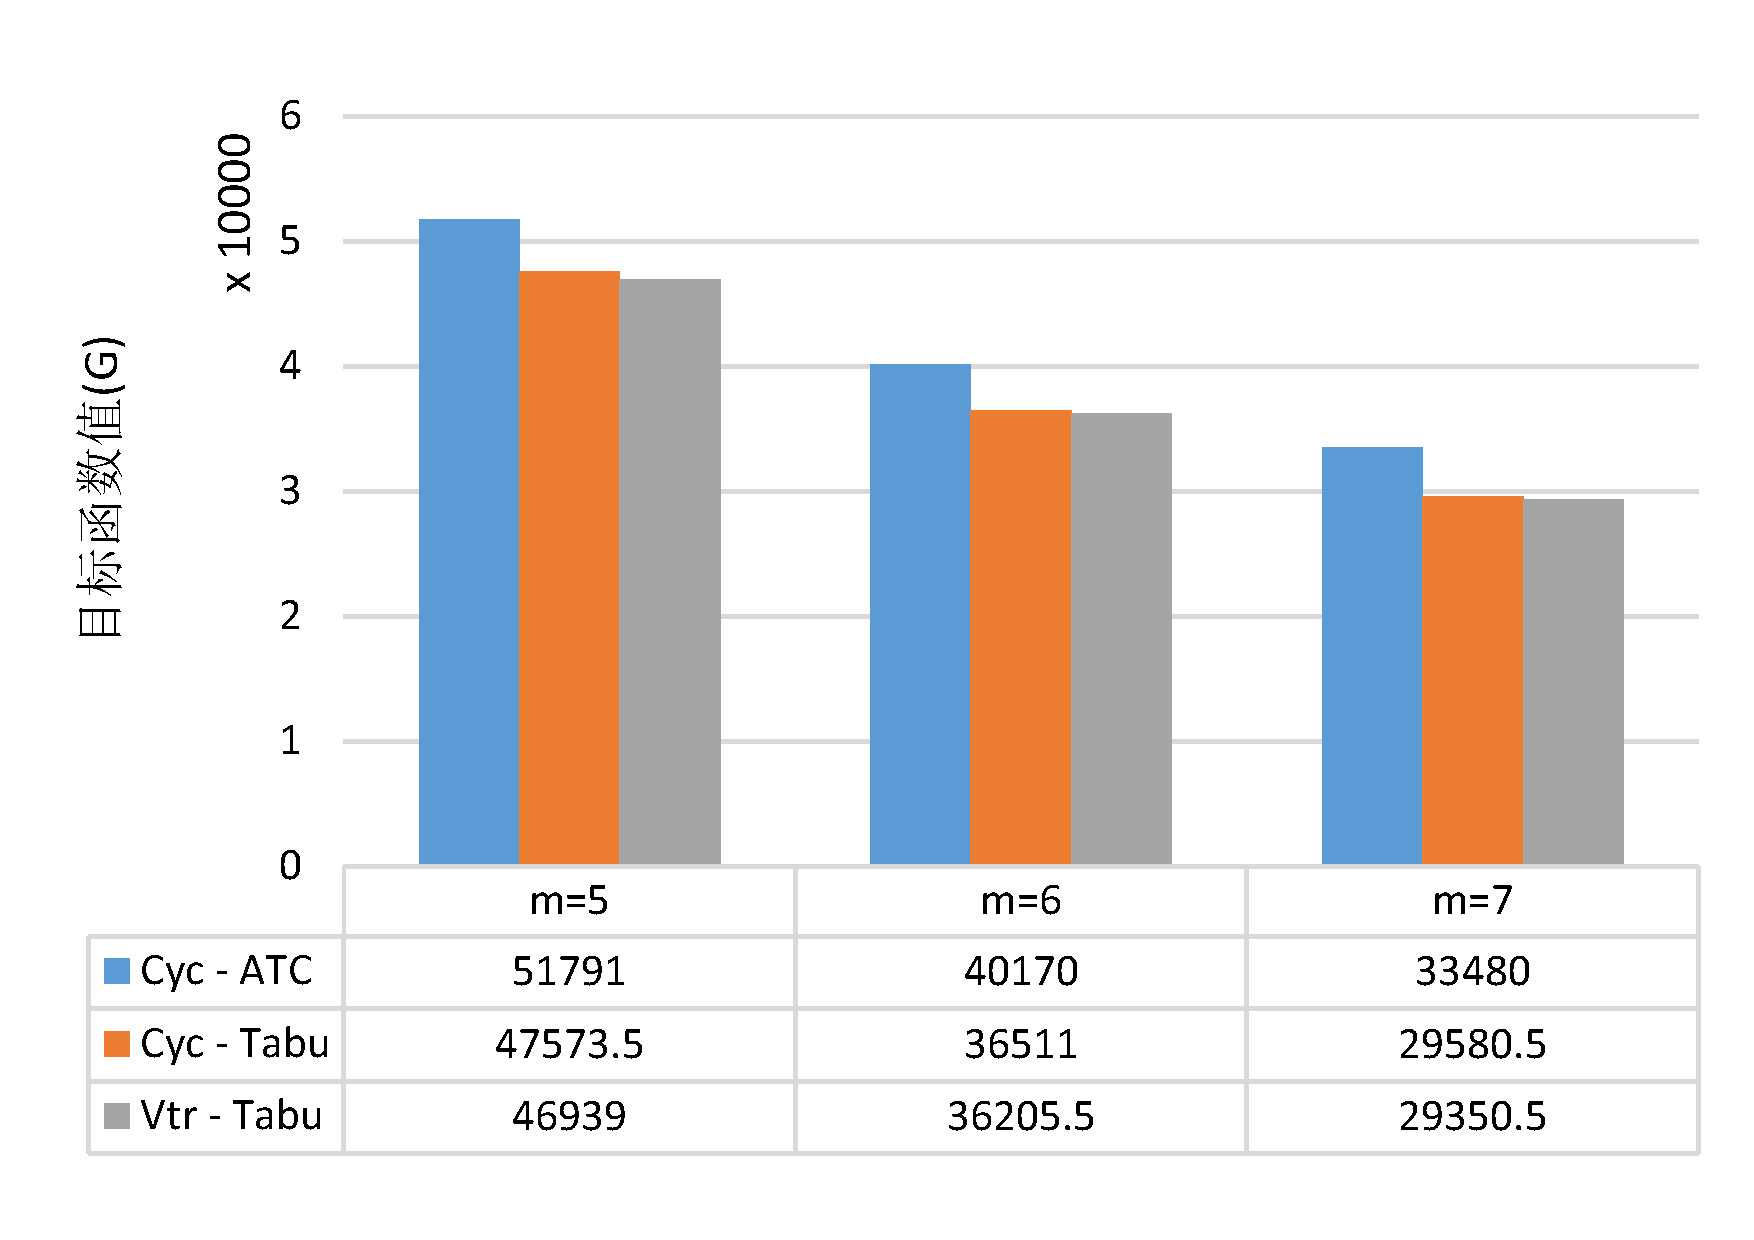
\includegraphics[height = 6cm, angle = -90]{basic_05_70}}\\
\subfloat[$n = 100$]{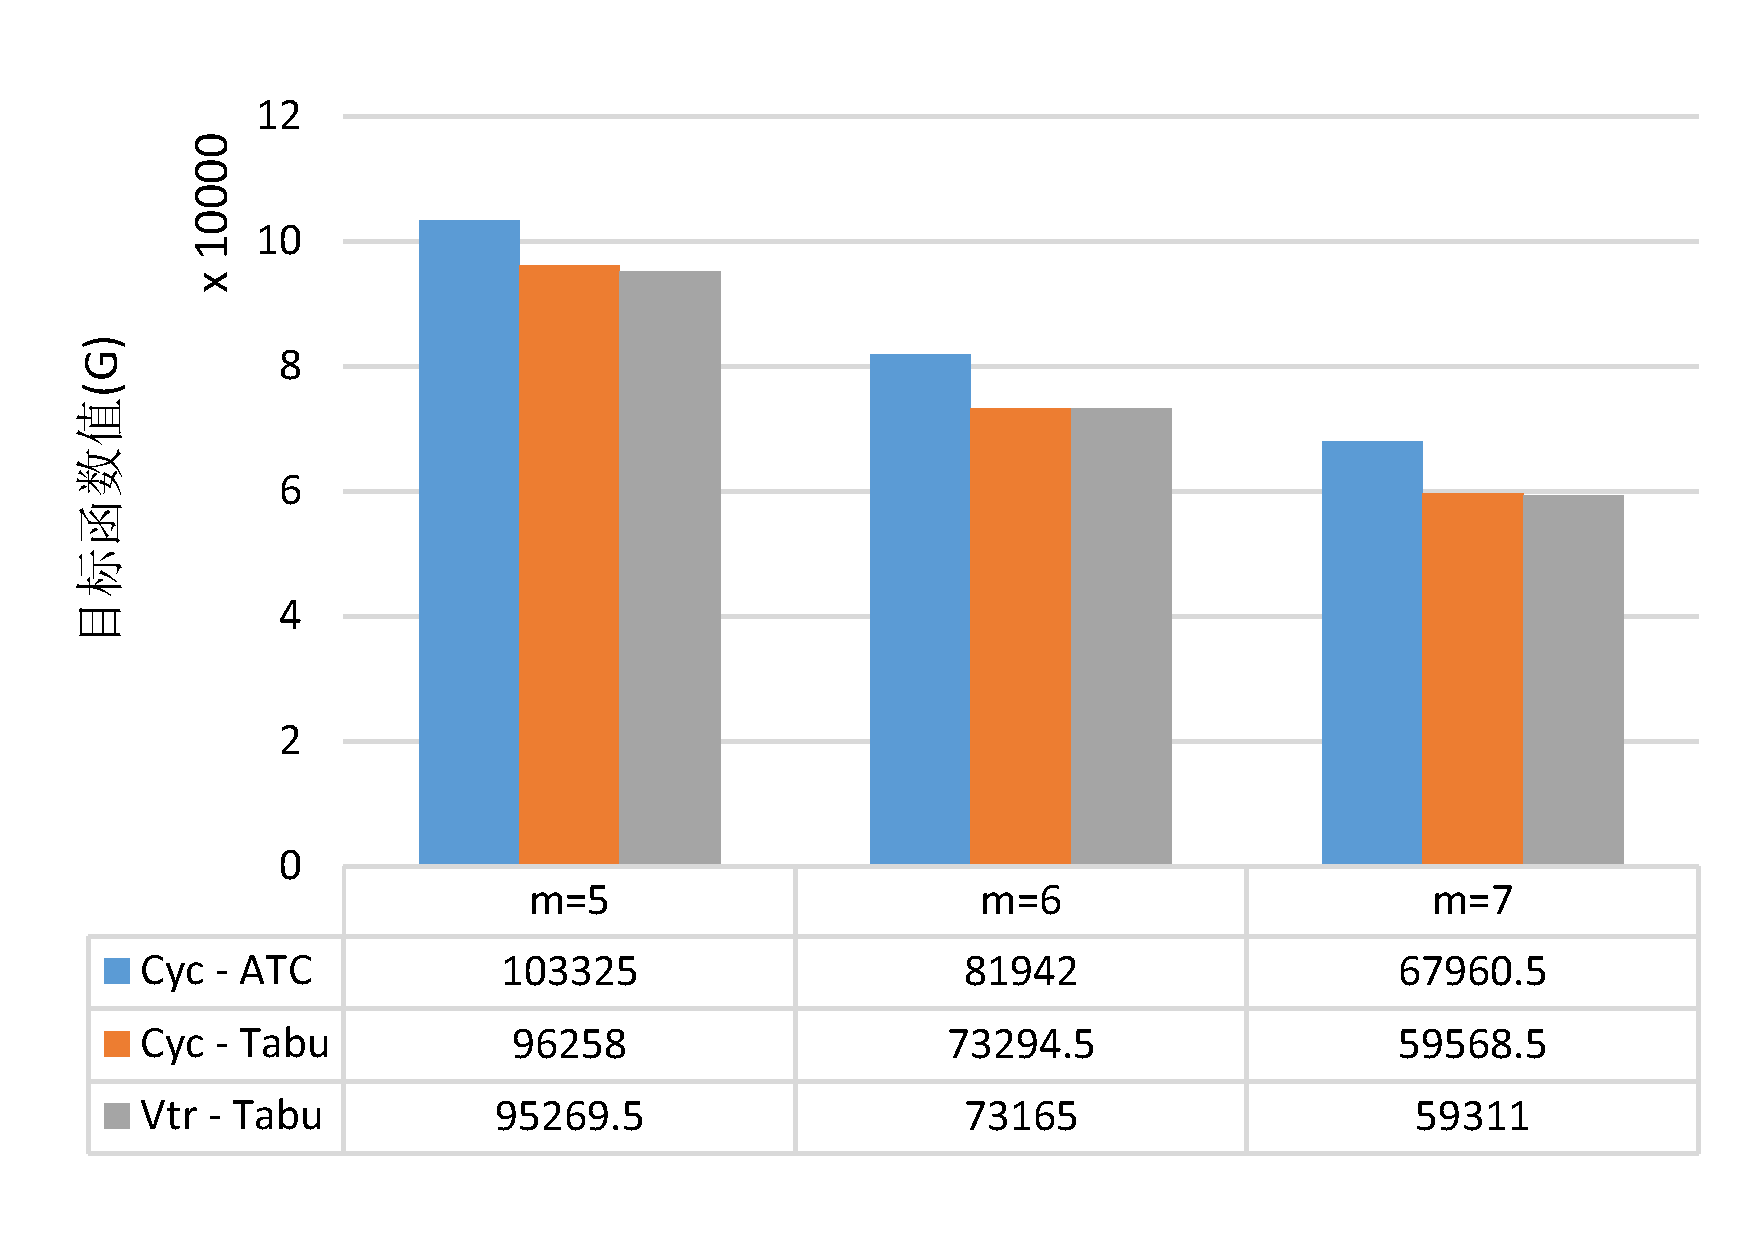
\includegraphics[height = 6cm, angle = -90]{basic_05_100}}
\subfloat[$n = 150$]{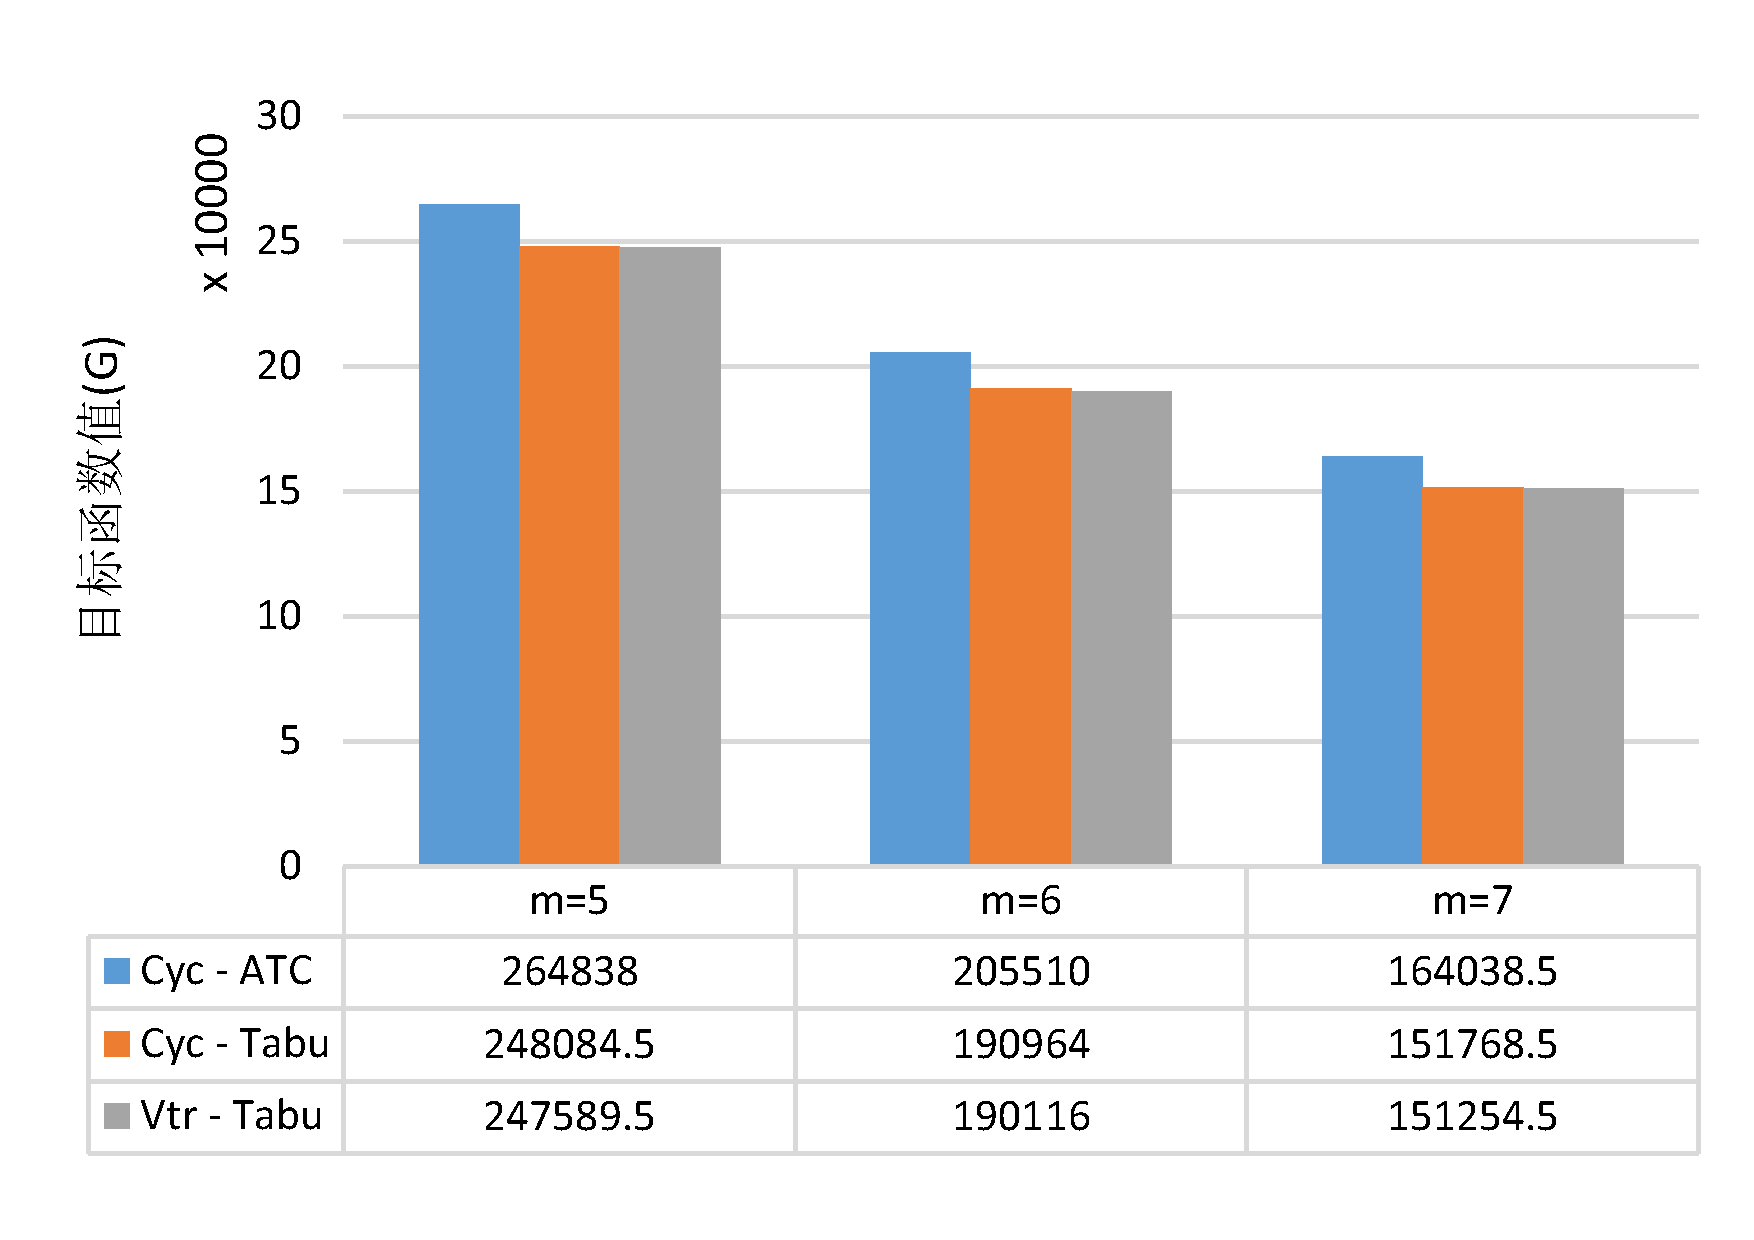
\includegraphics[height = 6cm, angle = -90]{basic_05_150}}
\subfloat[$n = 200$]{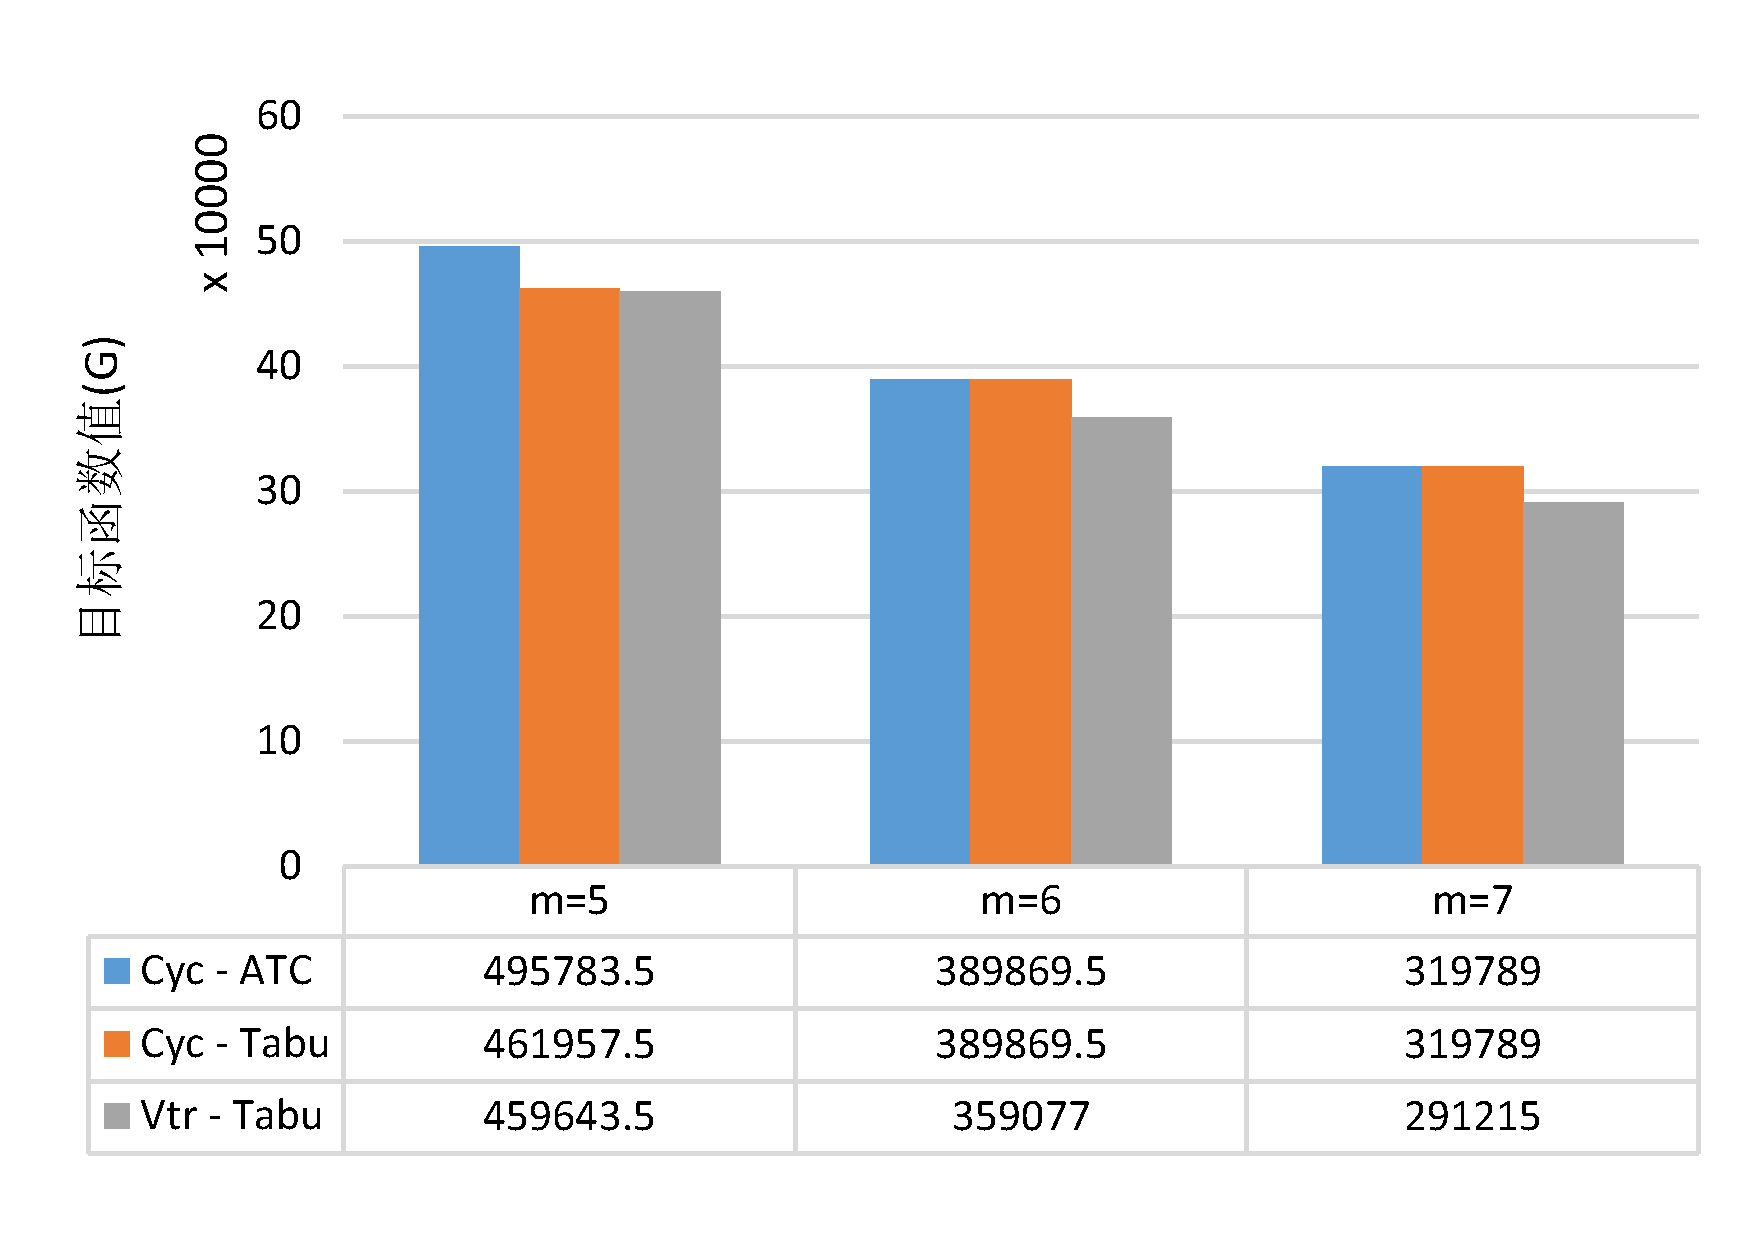
\includegraphics[height = 6cm, angle = -90]{basic_05_200}}
\subfloat[$n = 300$]{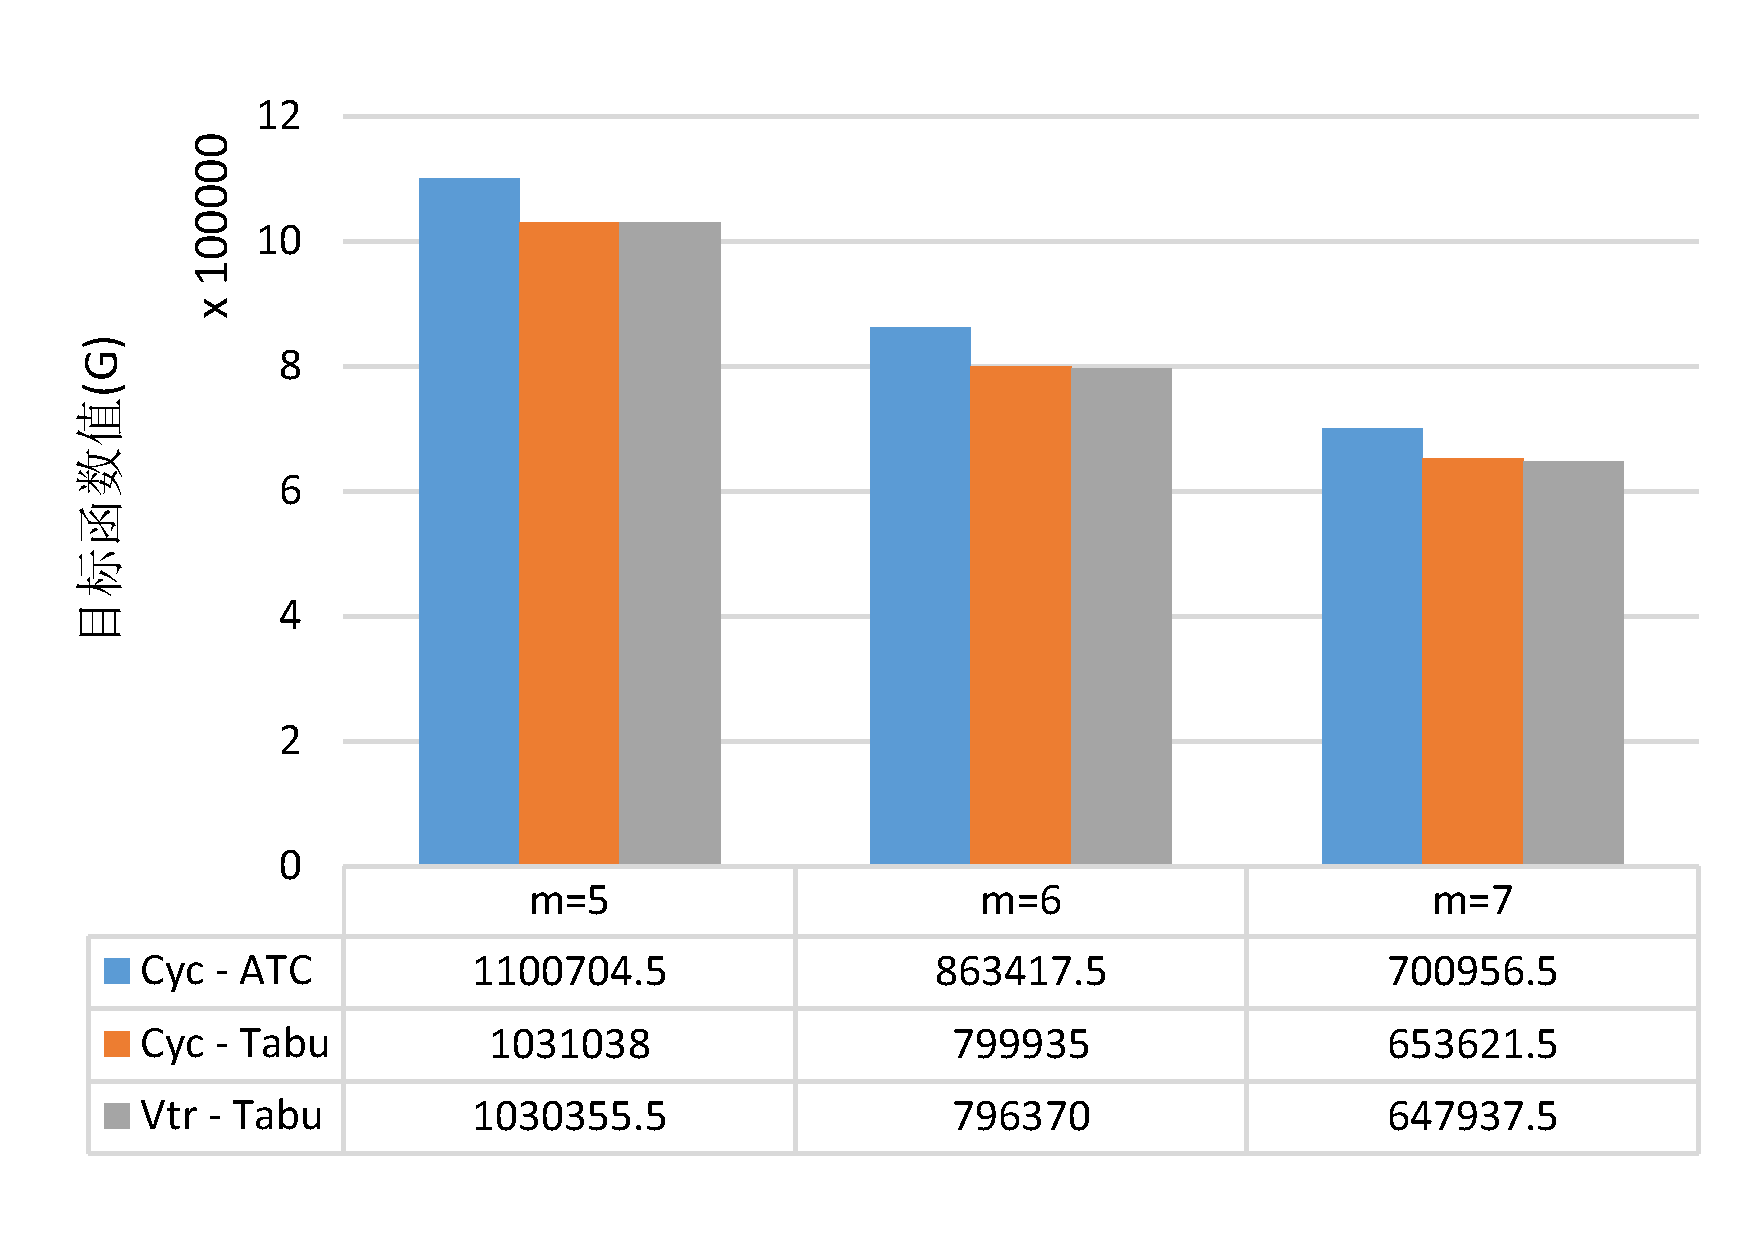
\includegraphics[height = 6cm, angle = -90]{basic_05_300}}\\
\subfloat[$n = 500$]{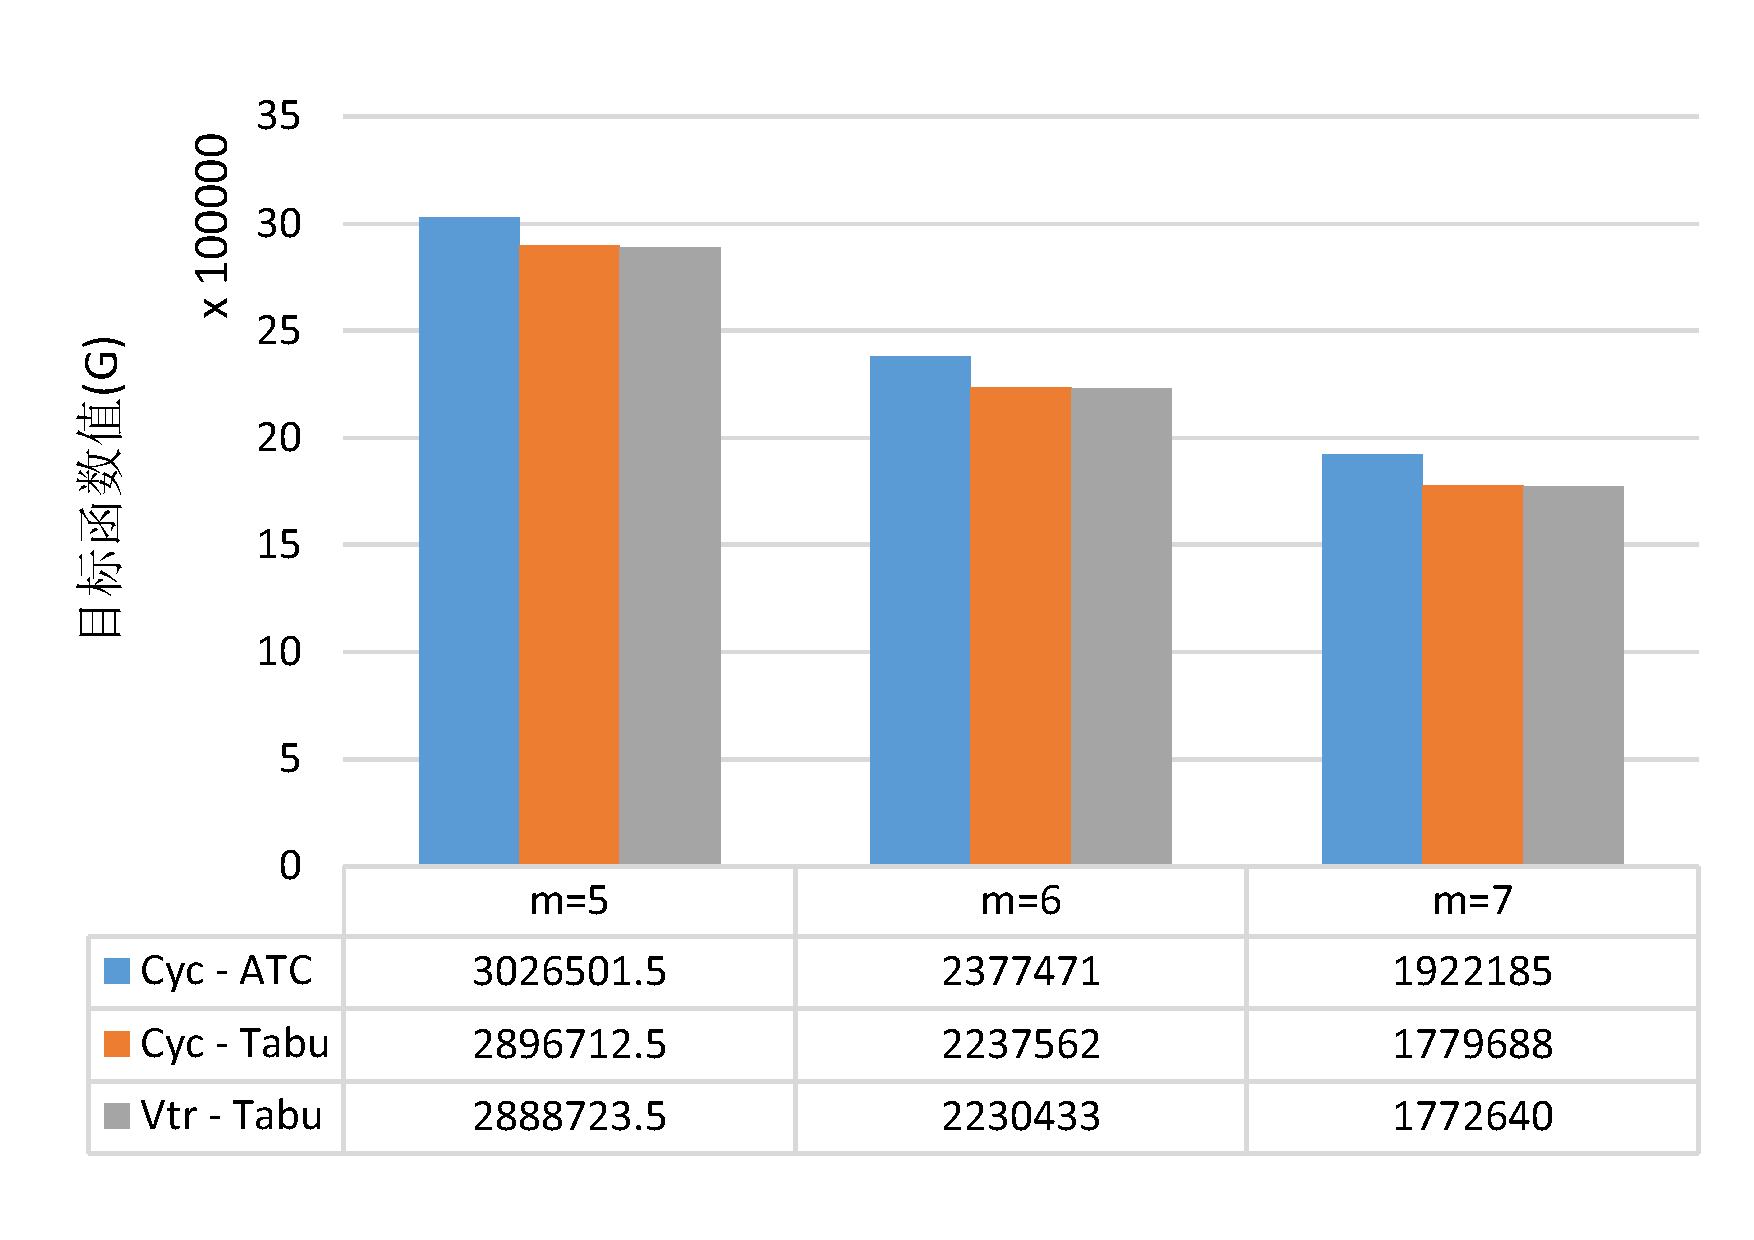
\includegraphics[height = 6cm, angle = -90]{basic_05_500}}
\subfloat[$n = 750$]{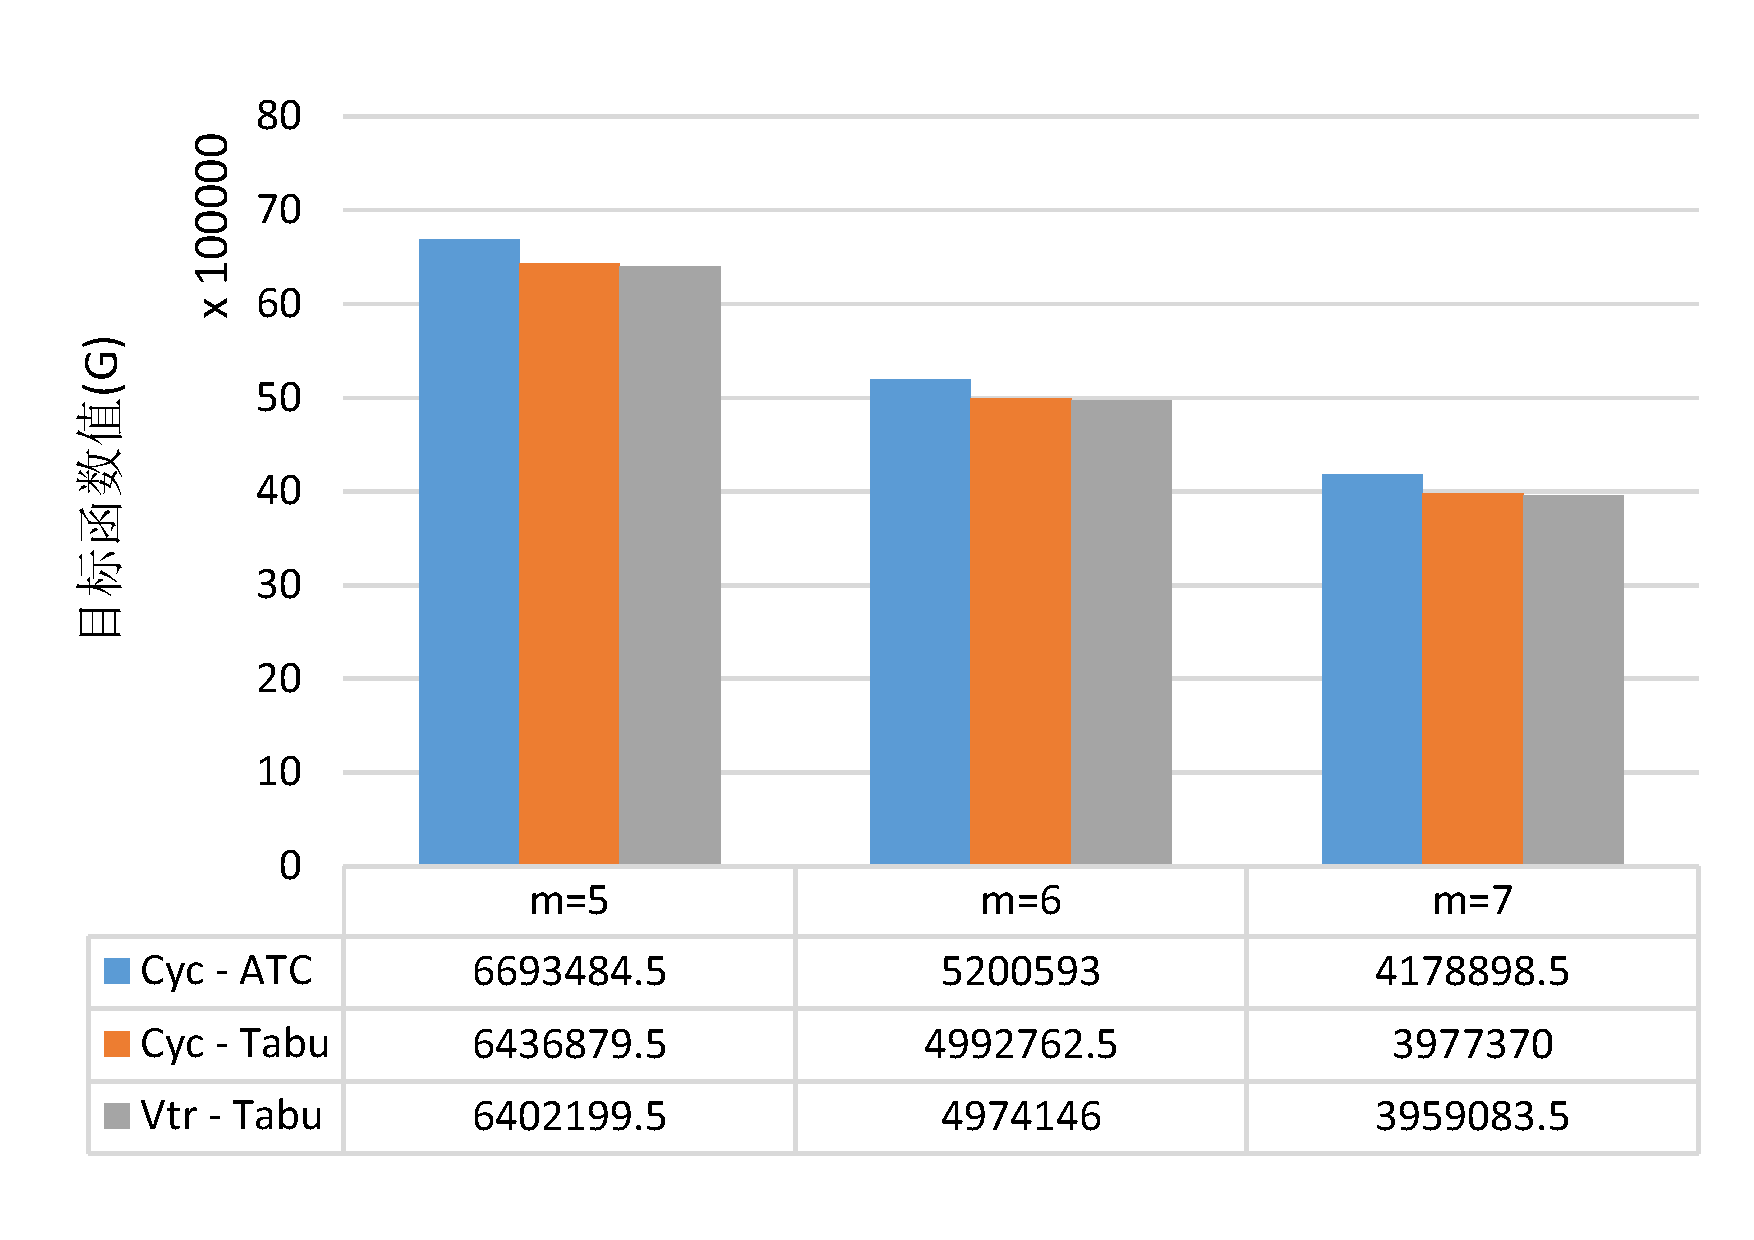
\includegraphics[height = 6cm, angle = -90]{basic_05_750}}
\subfloat[$n = 1000$]{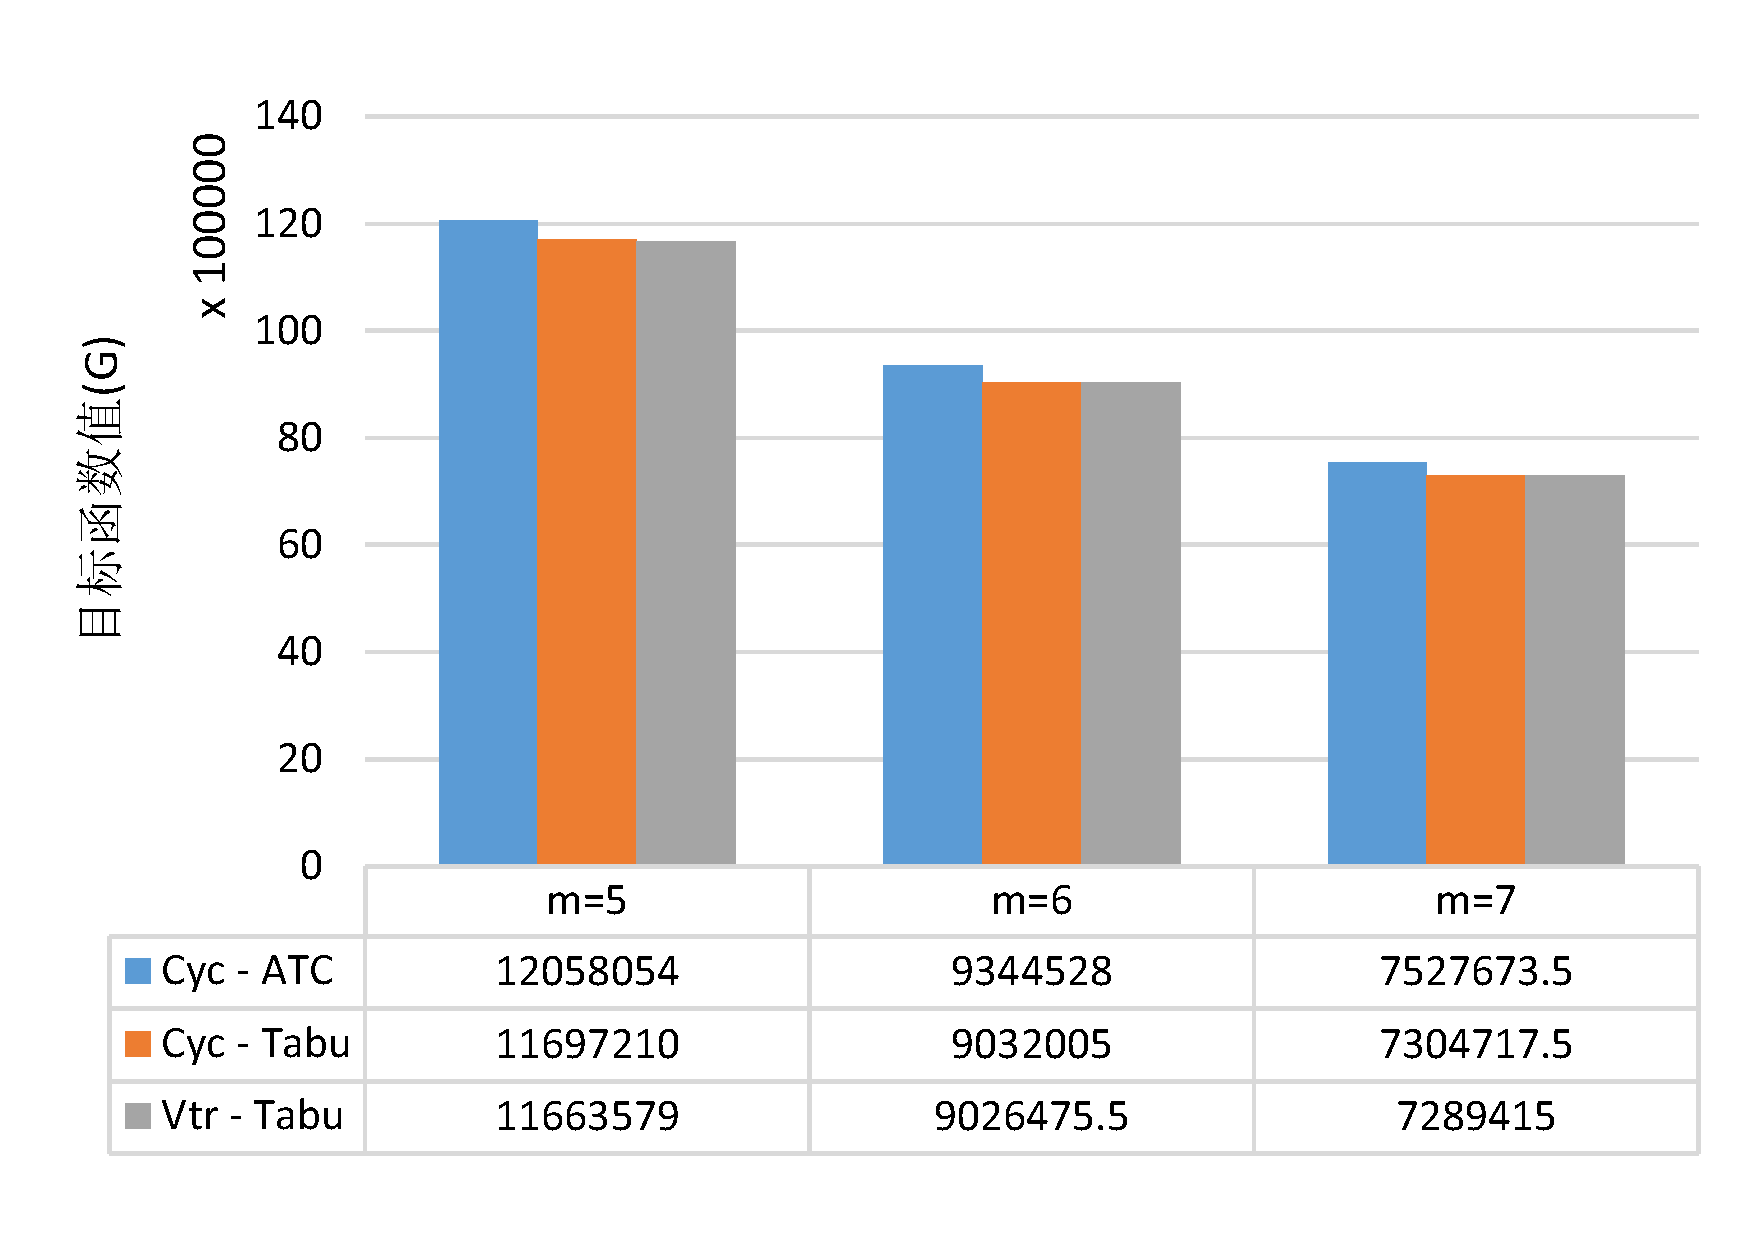
\includegraphics[height = 6cm, angle = -90]{basic_05_1000}}
\caption{\label{fig:result2}模型$1$的Cyc -- ATC、Cyc -- Tabu、Vtr -- Tabu 算法求解目标函数值比较$(\lambda_1 = 0.5)$}
\end{sidewaysfigure}

\begin{sidewaysfigure}
\centering
\subfloat[$n = 20$]{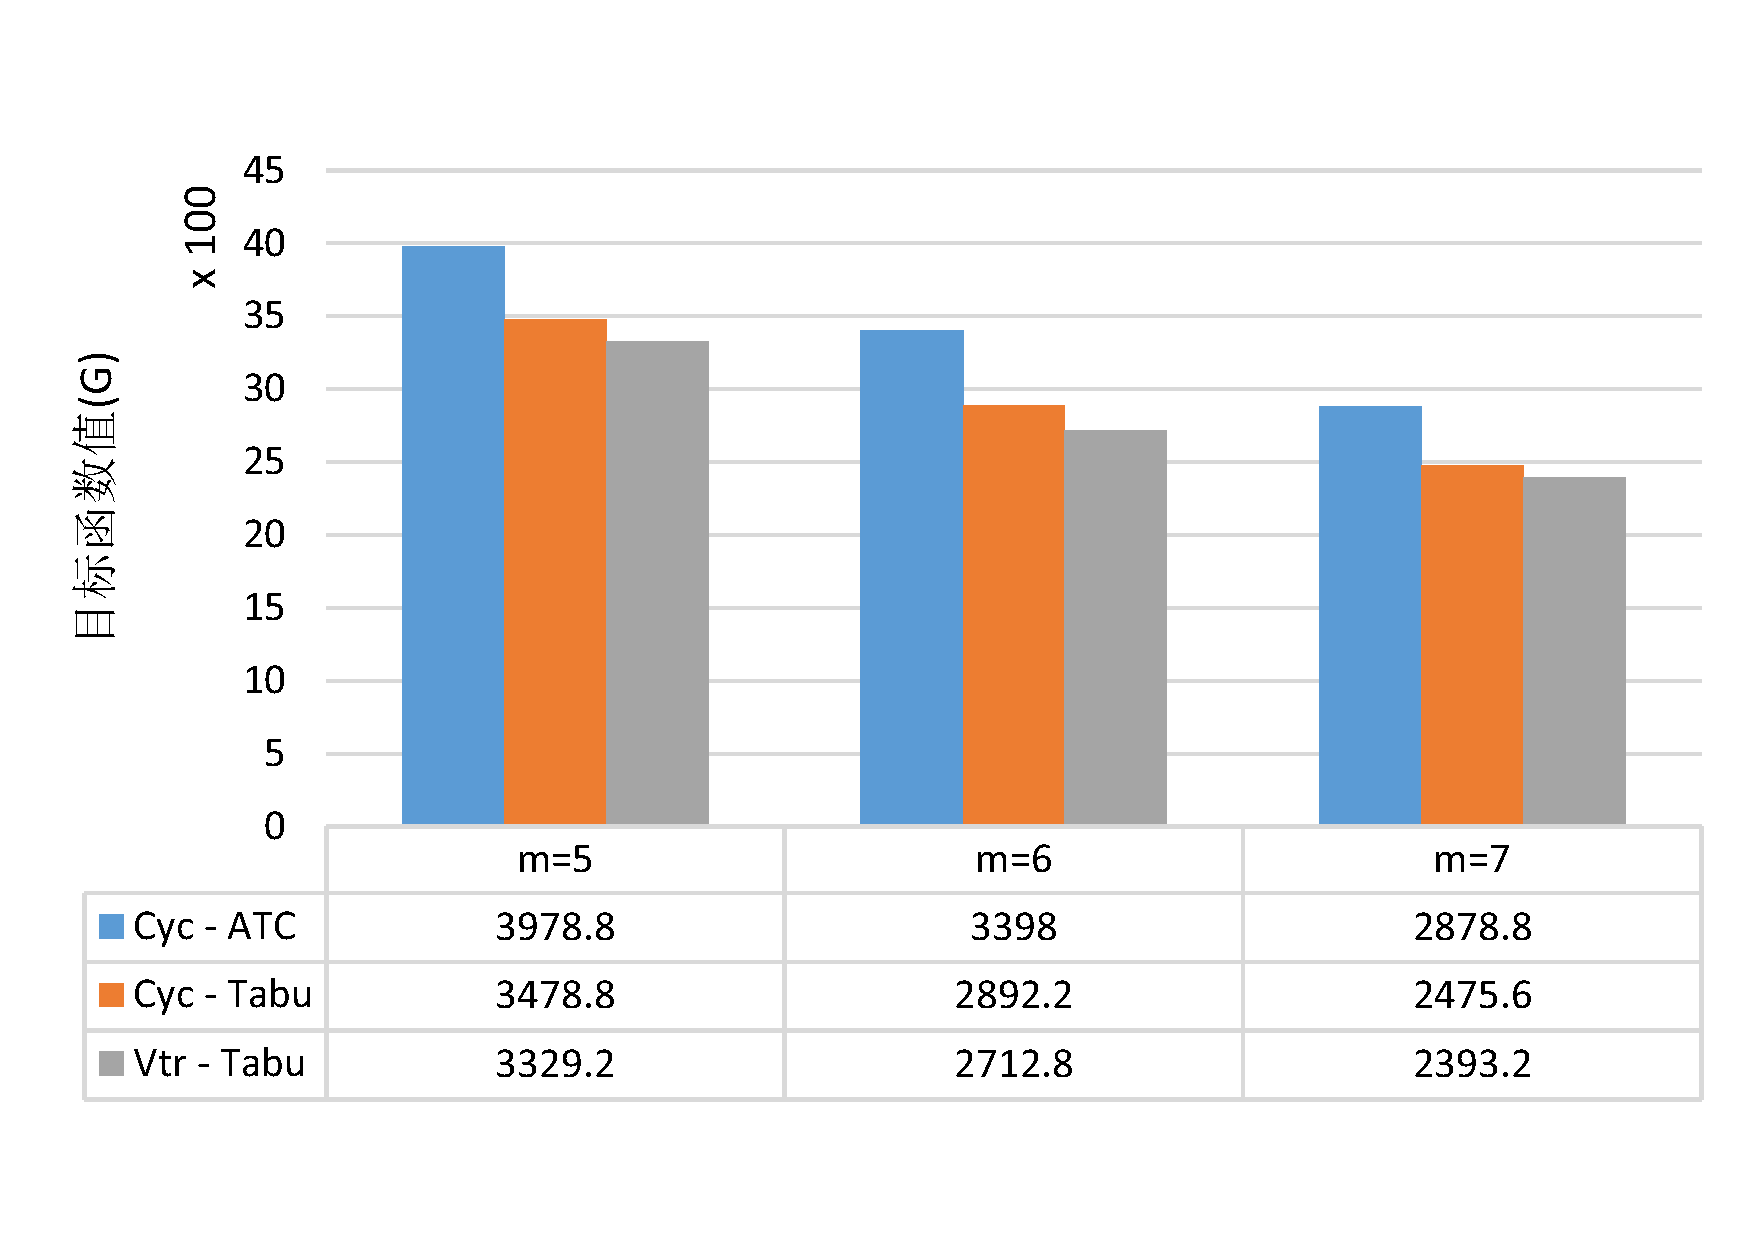
\includegraphics[height = 6cm, angle = -90]{basic_06_20}}
\subfloat[$n = 30$]{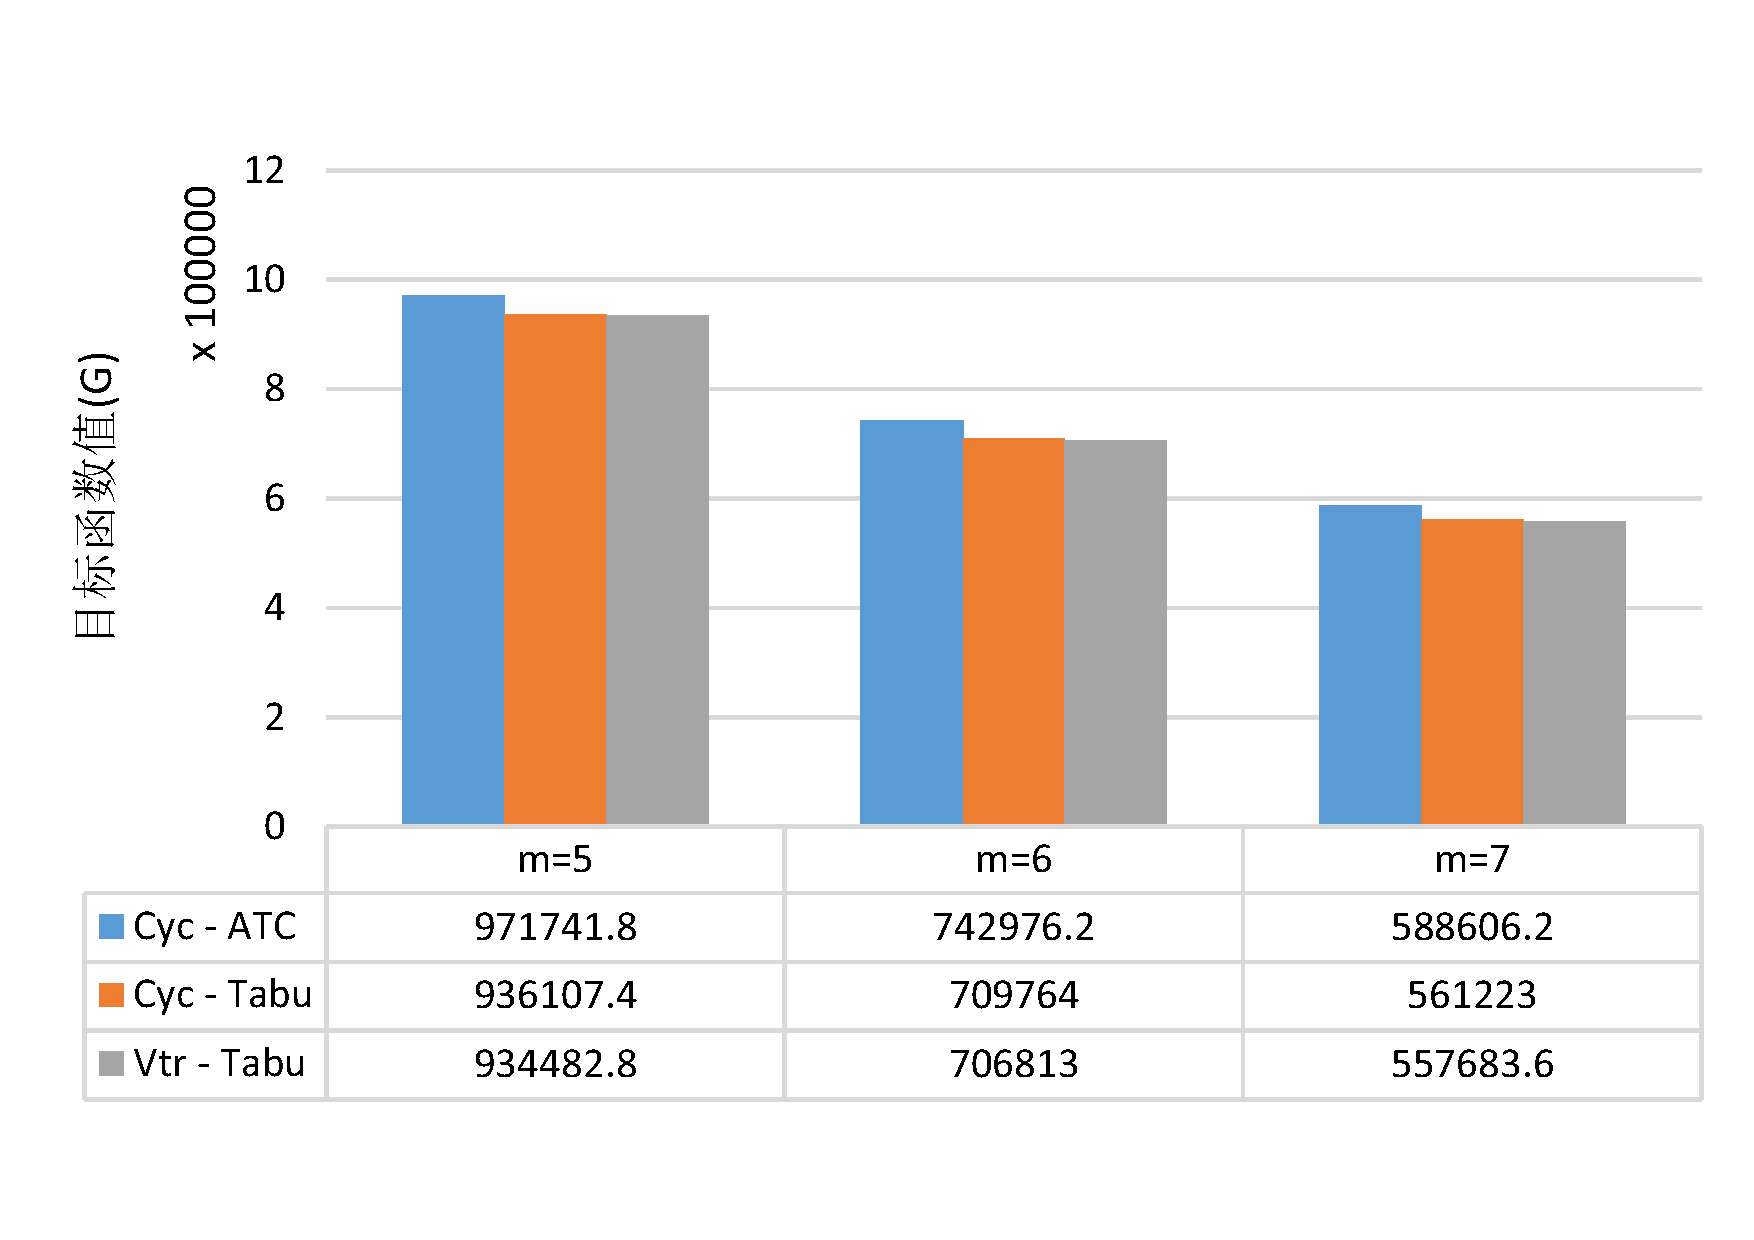
\includegraphics[height = 6cm, angle = -90]{basic_06_300}}
\subfloat[$n = 50$]{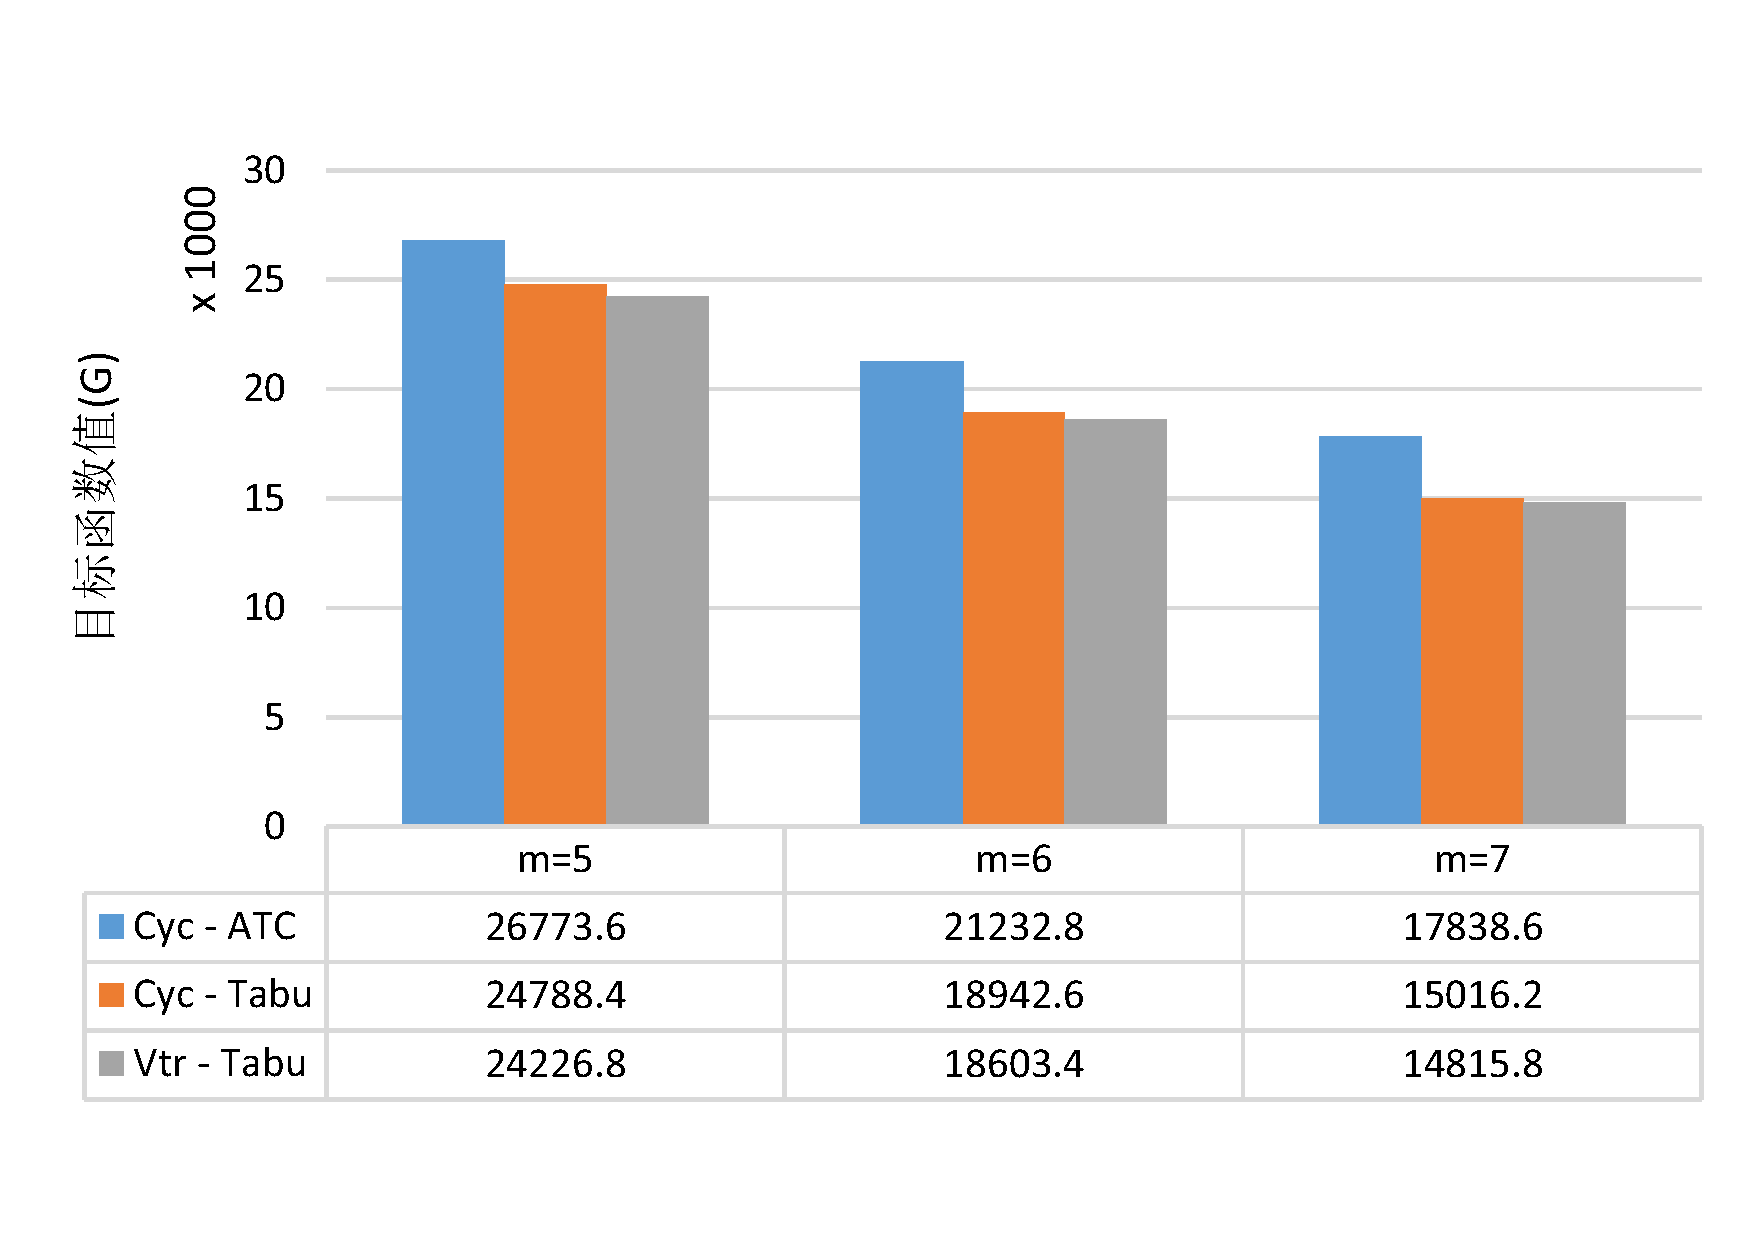
\includegraphics[height = 6cm, angle = -90]{basic_06_50}}
\subfloat[$n = 70$]{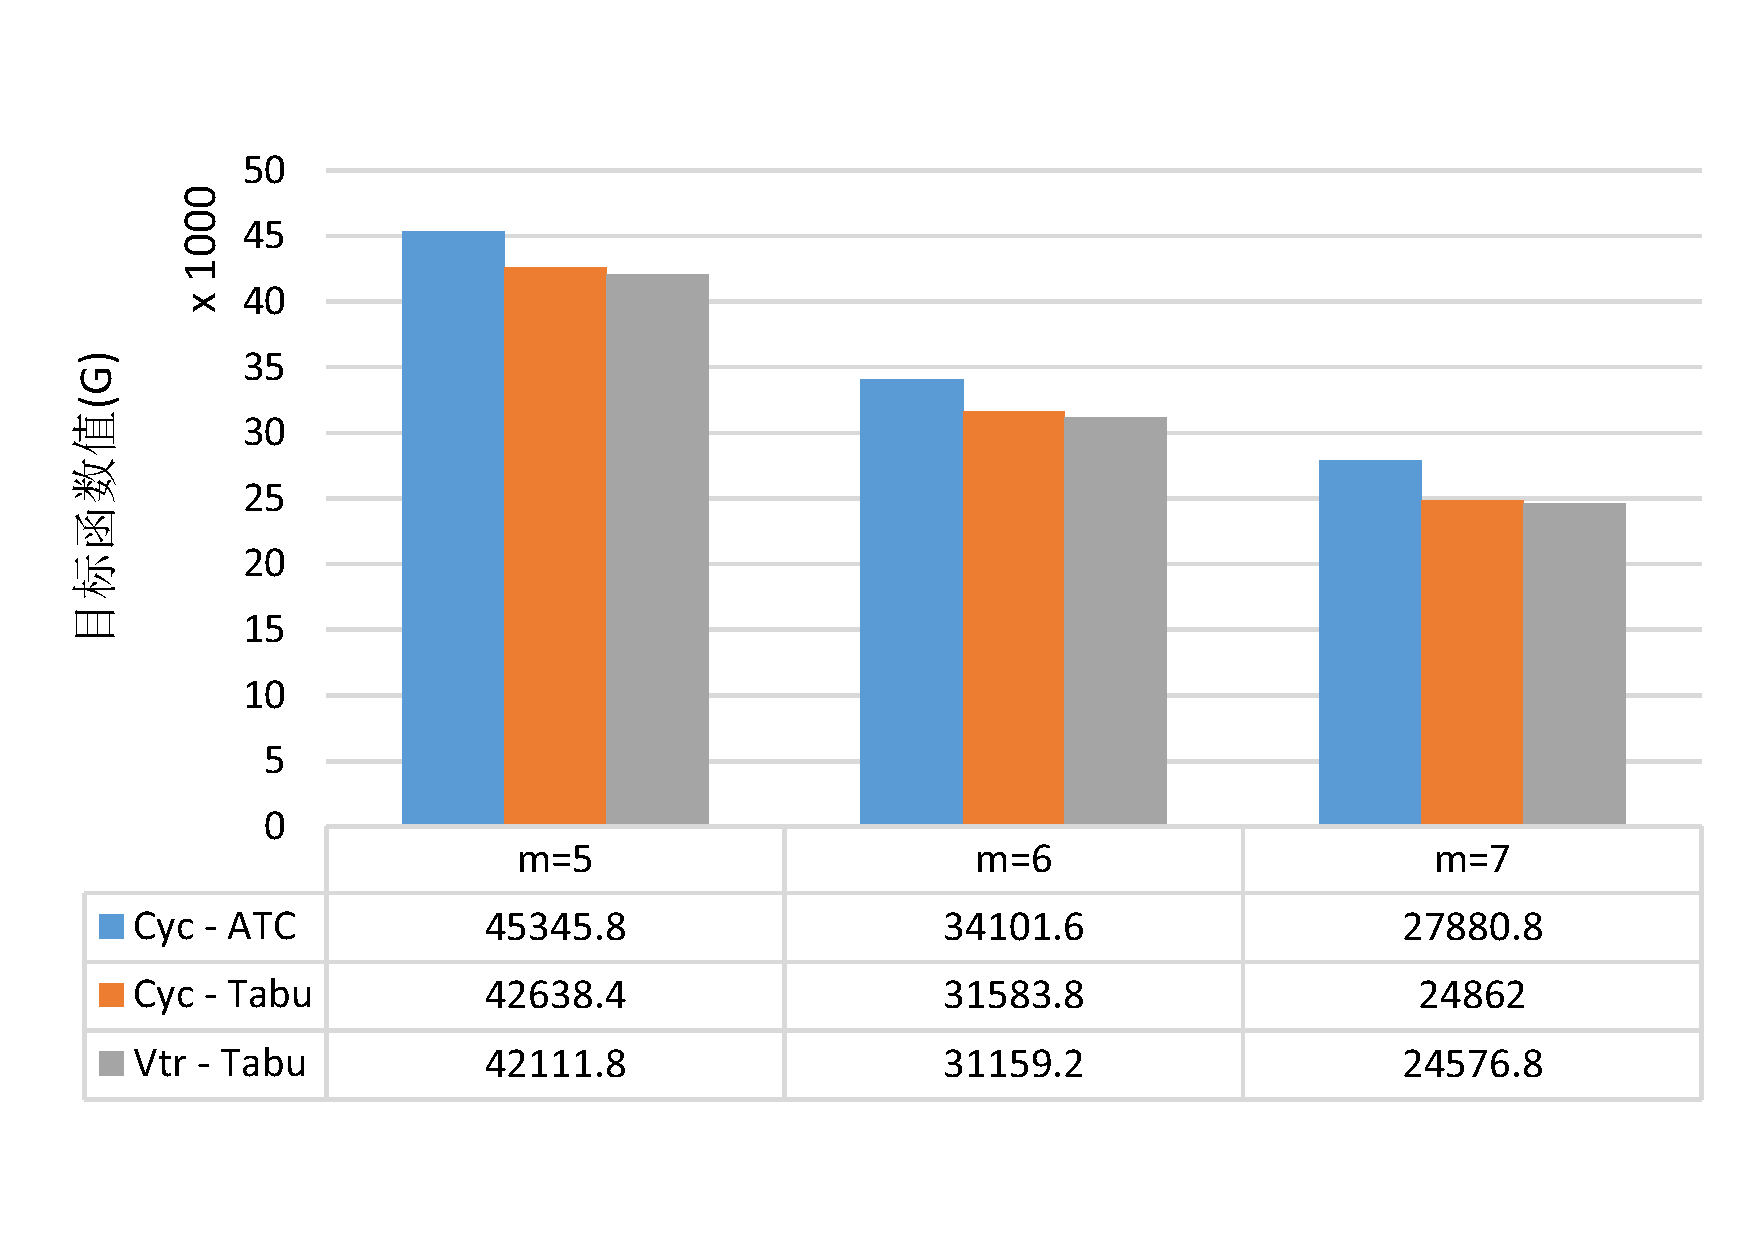
\includegraphics[height = 6cm, angle = -90]{basic_06_70}}\\
\subfloat[$n = 100$]{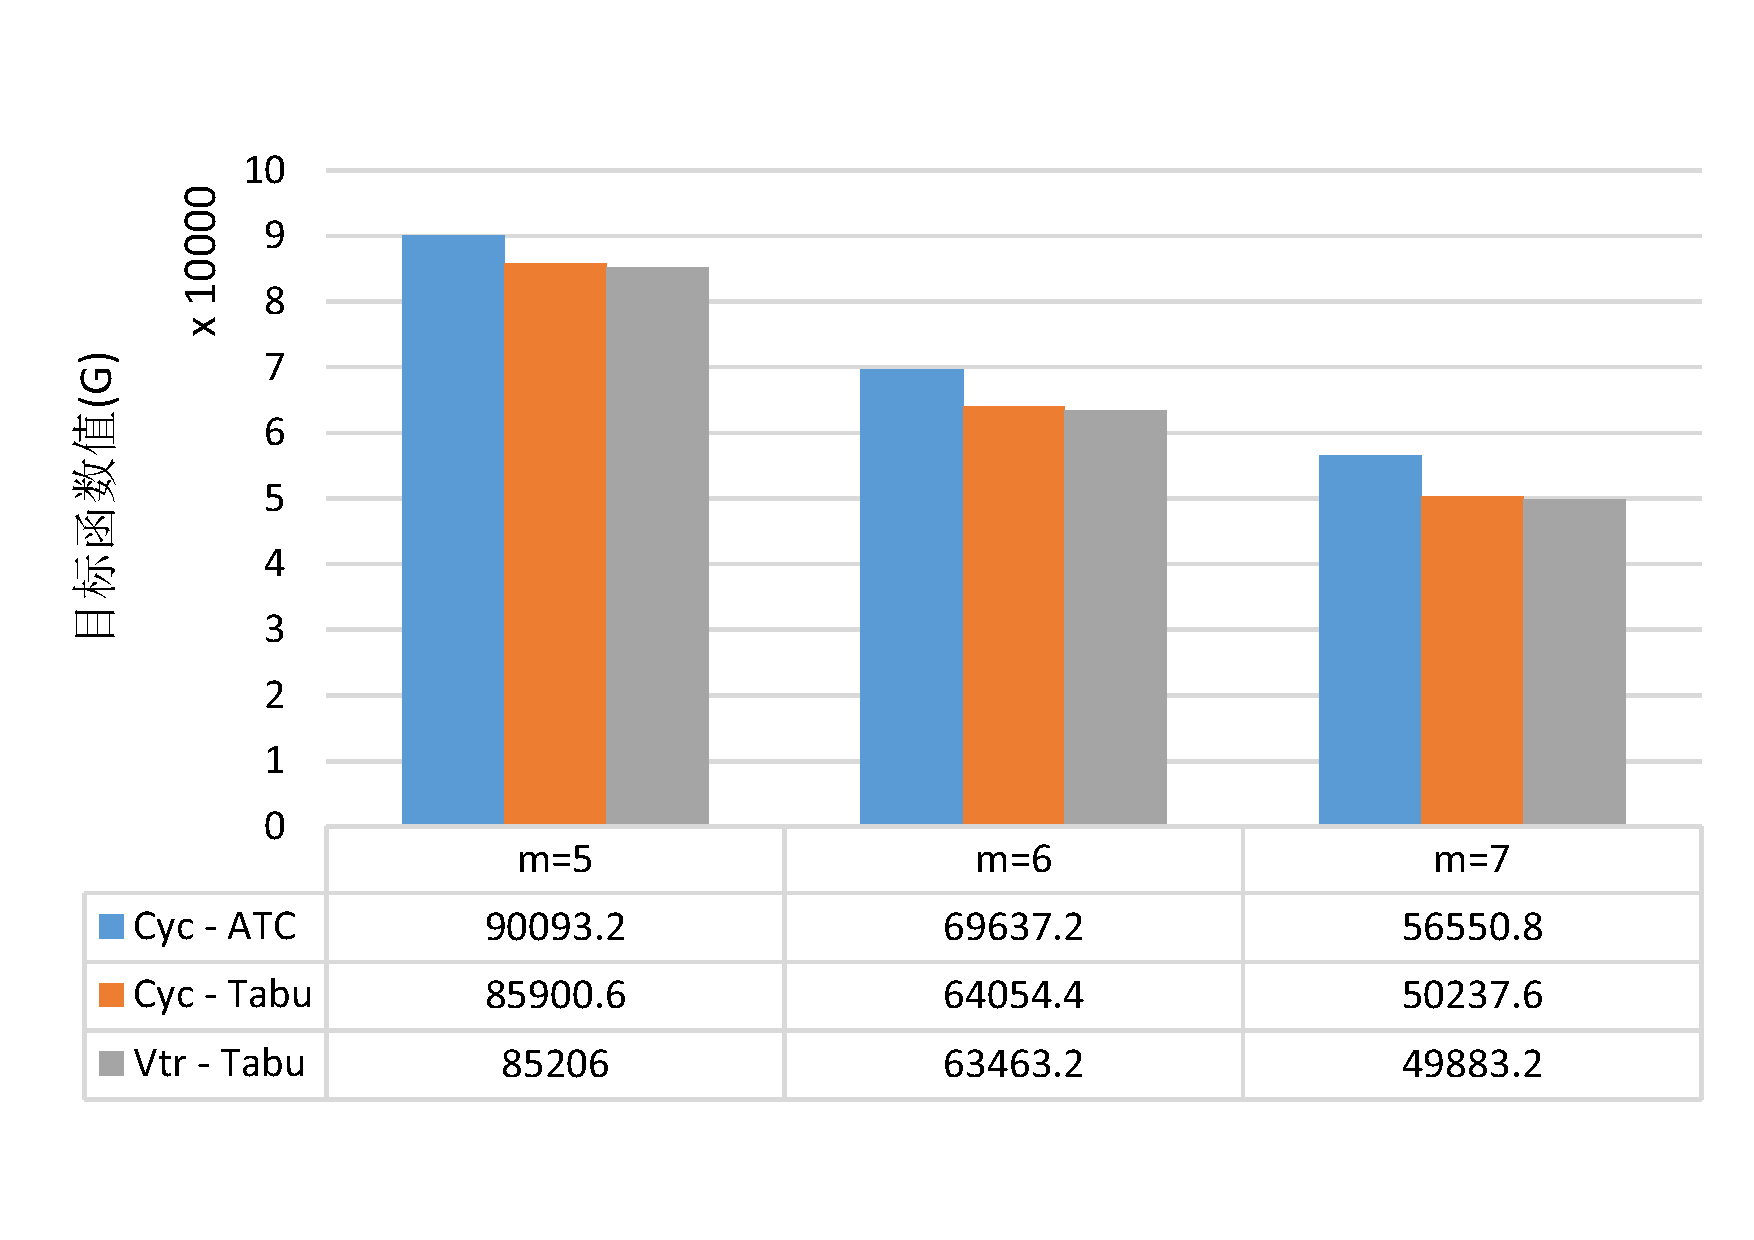
\includegraphics[height = 6cm, angle = -90]{basic_06_100}}
\subfloat[$n = 150$]{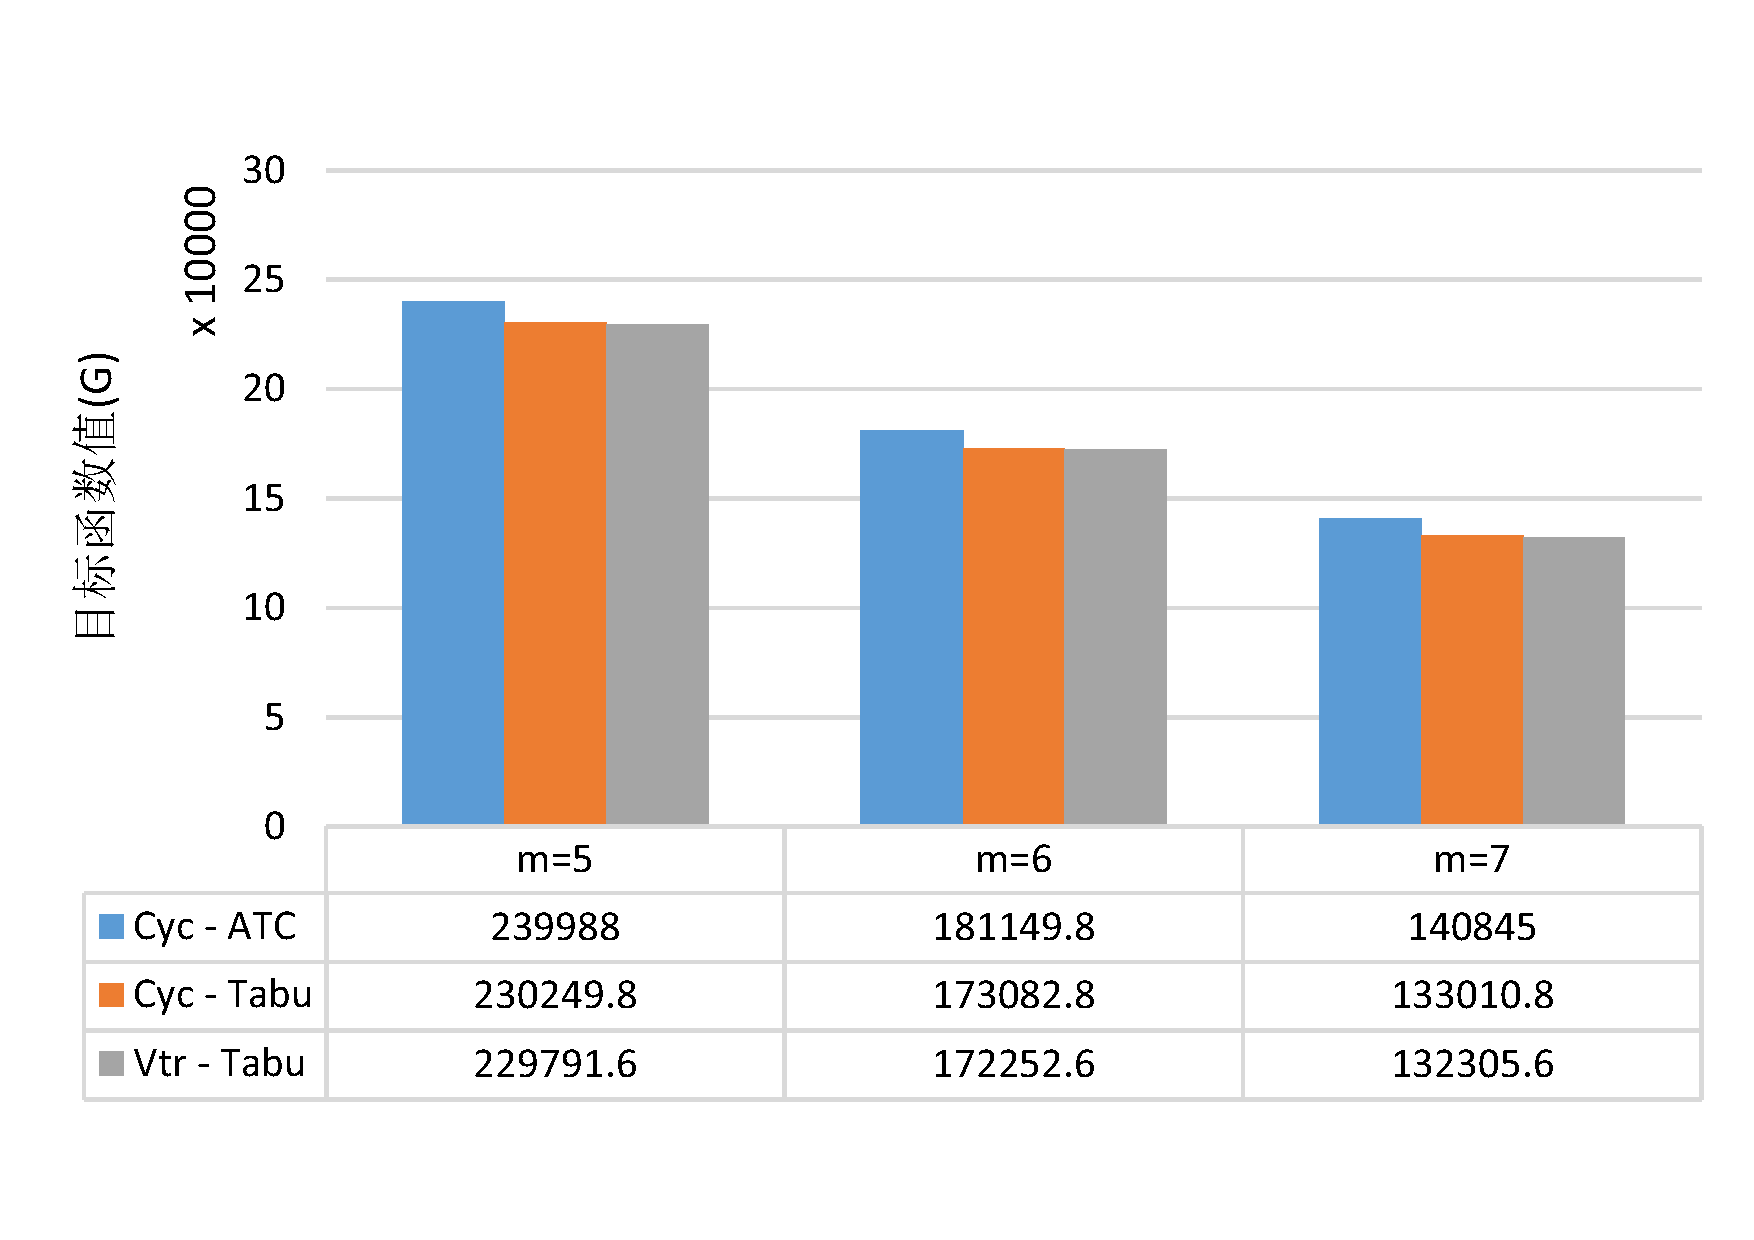
\includegraphics[height = 6cm, angle = -90]{basic_06_150}}
\subfloat[$n = 200$]{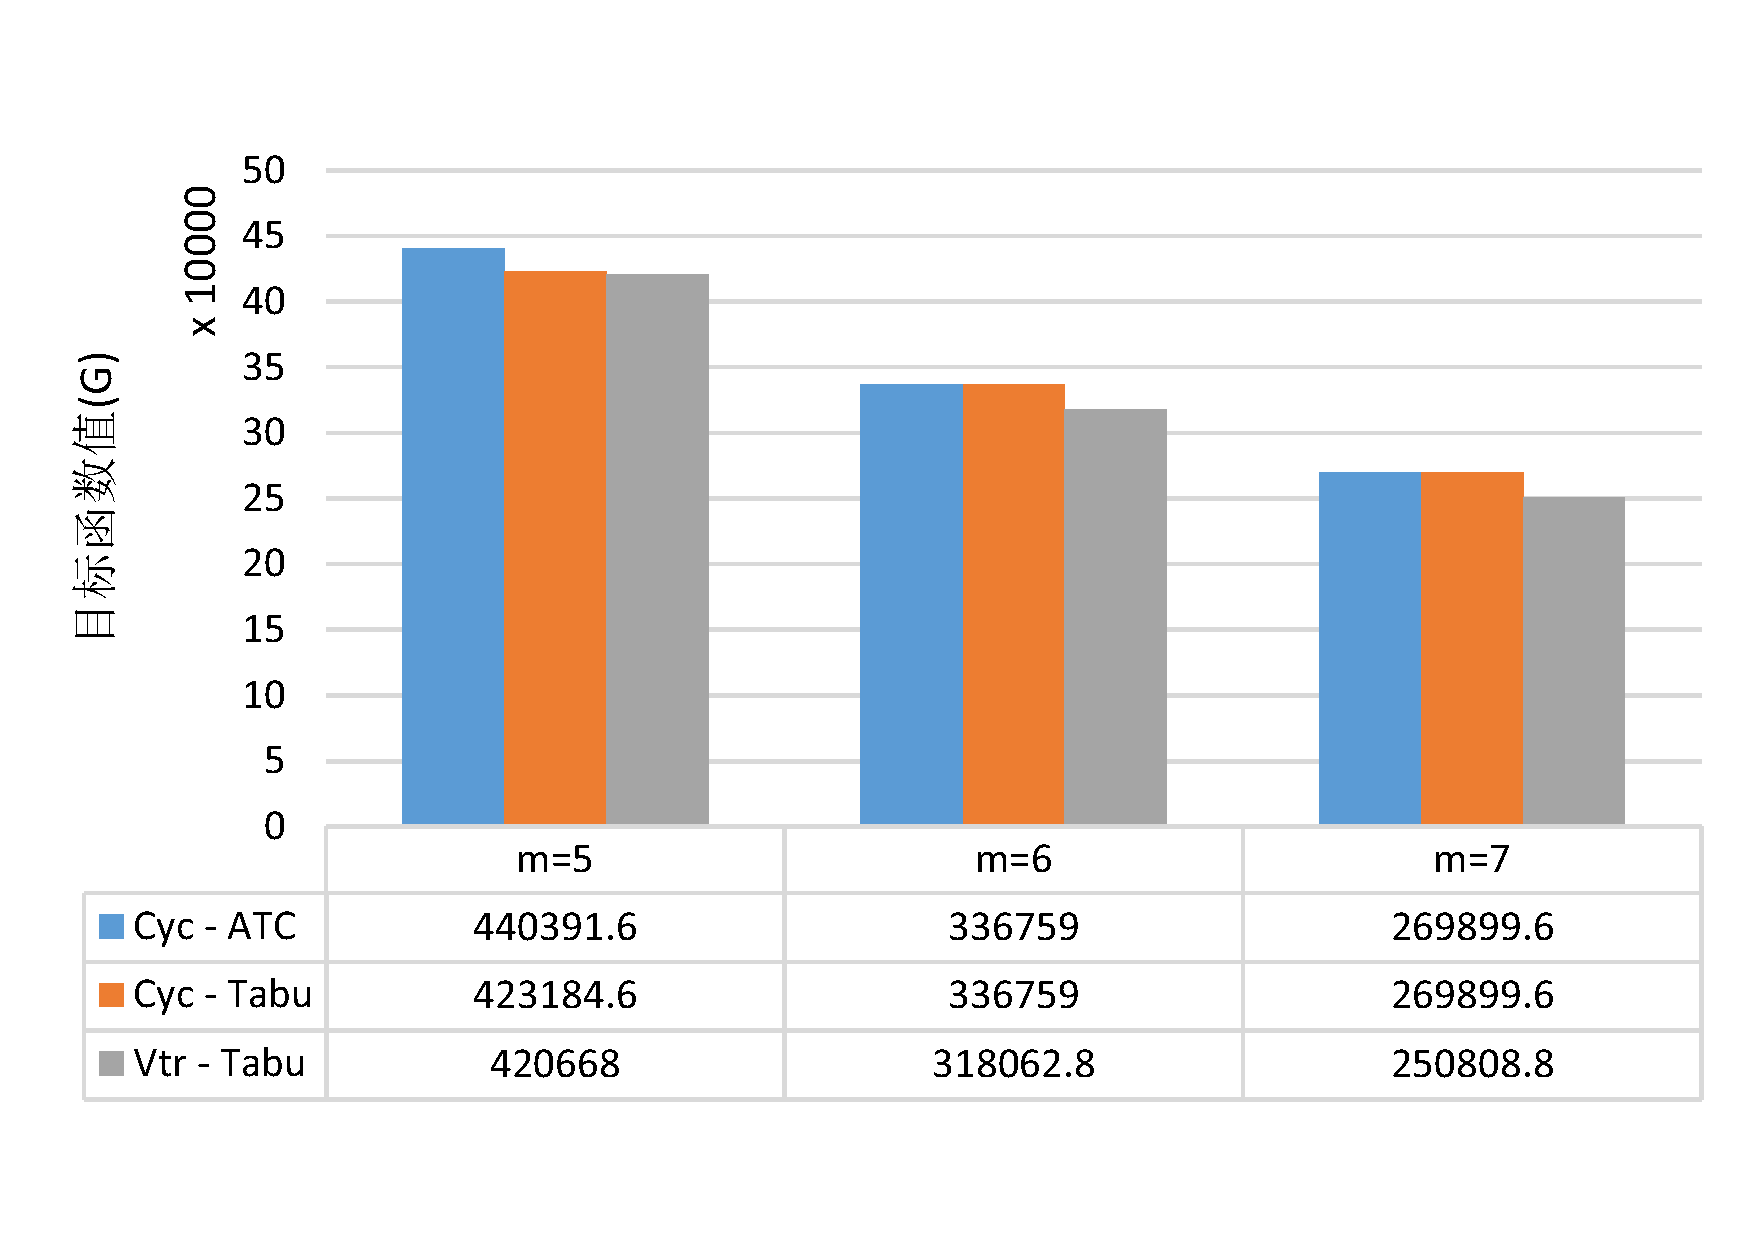
\includegraphics[height = 6cm, angle = -90]{basic_06_200}}
\subfloat[$n = 300$]{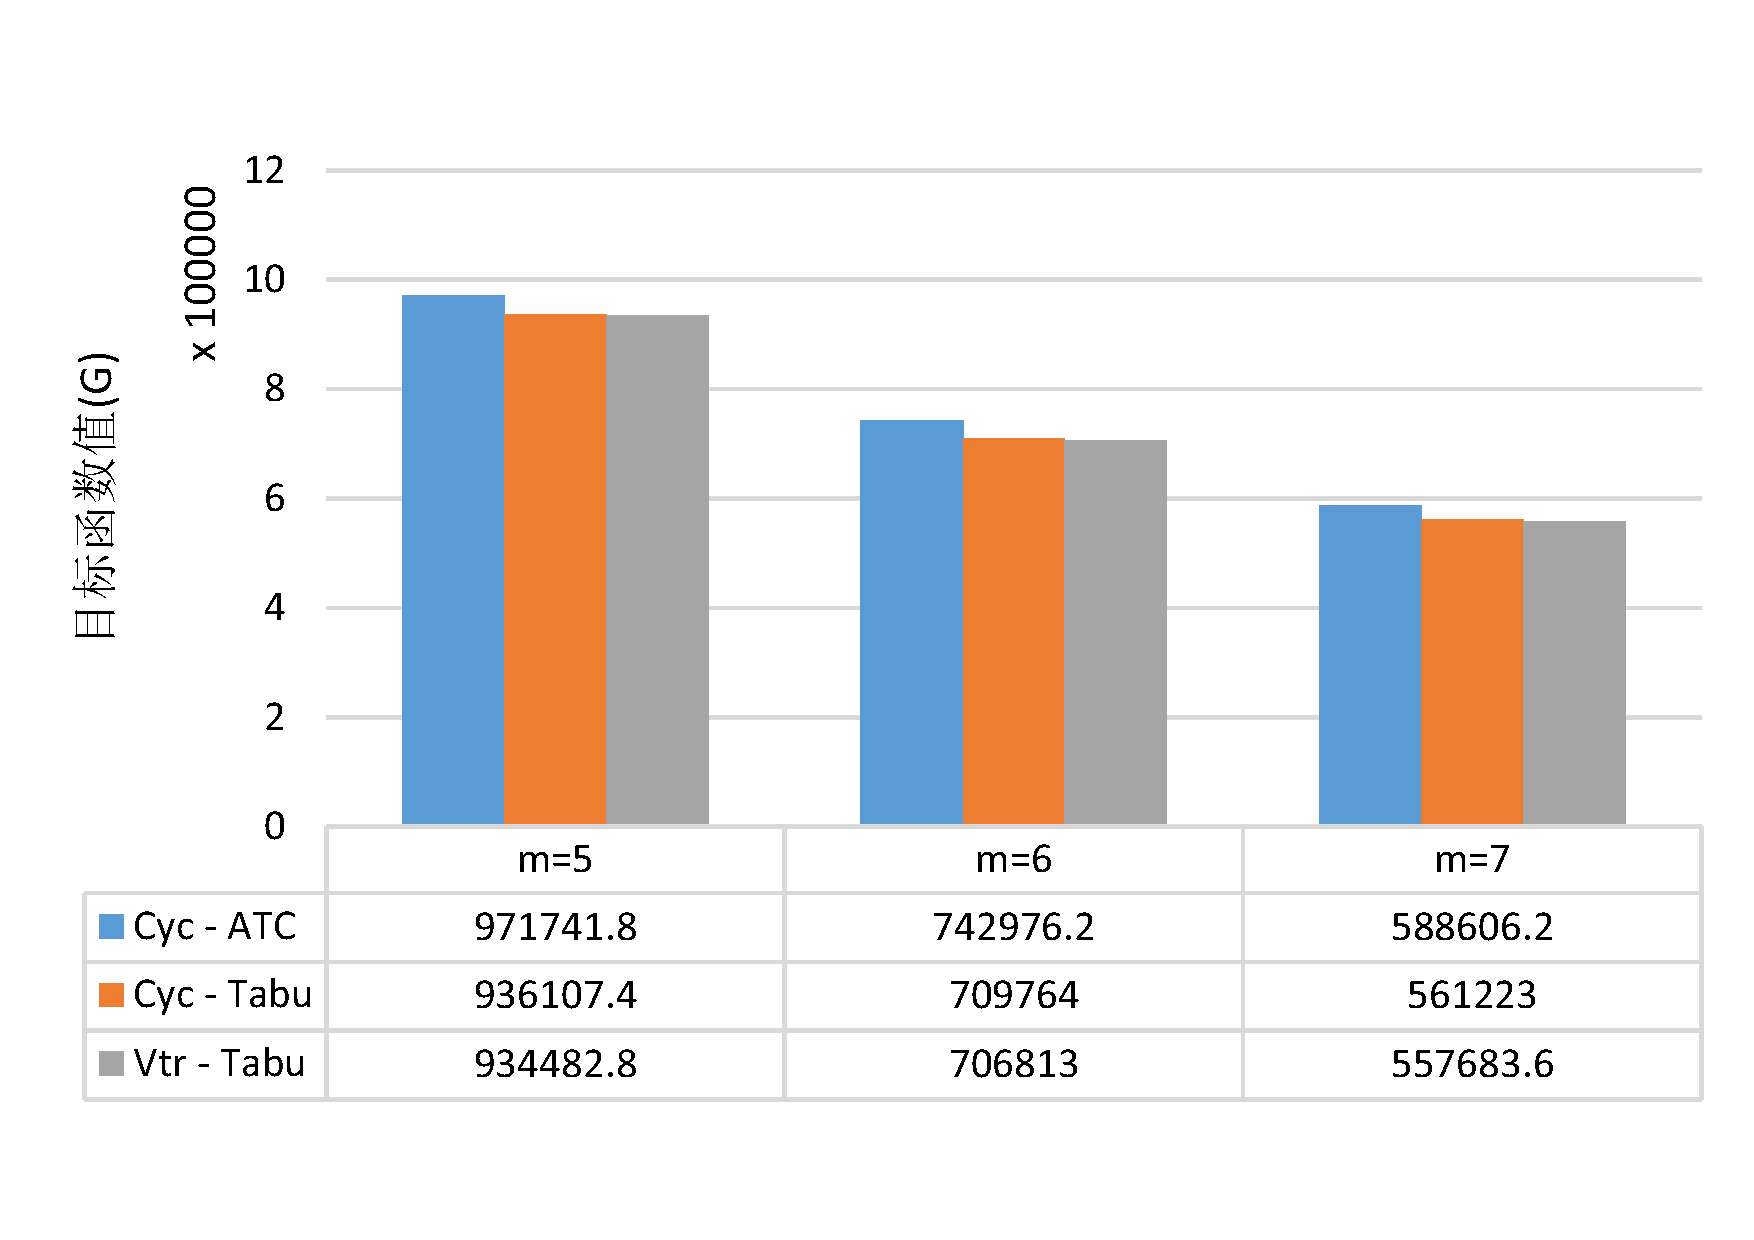
\includegraphics[height = 6cm, angle = -90]{basic_06_300}}\\
\subfloat[$n = 500$]{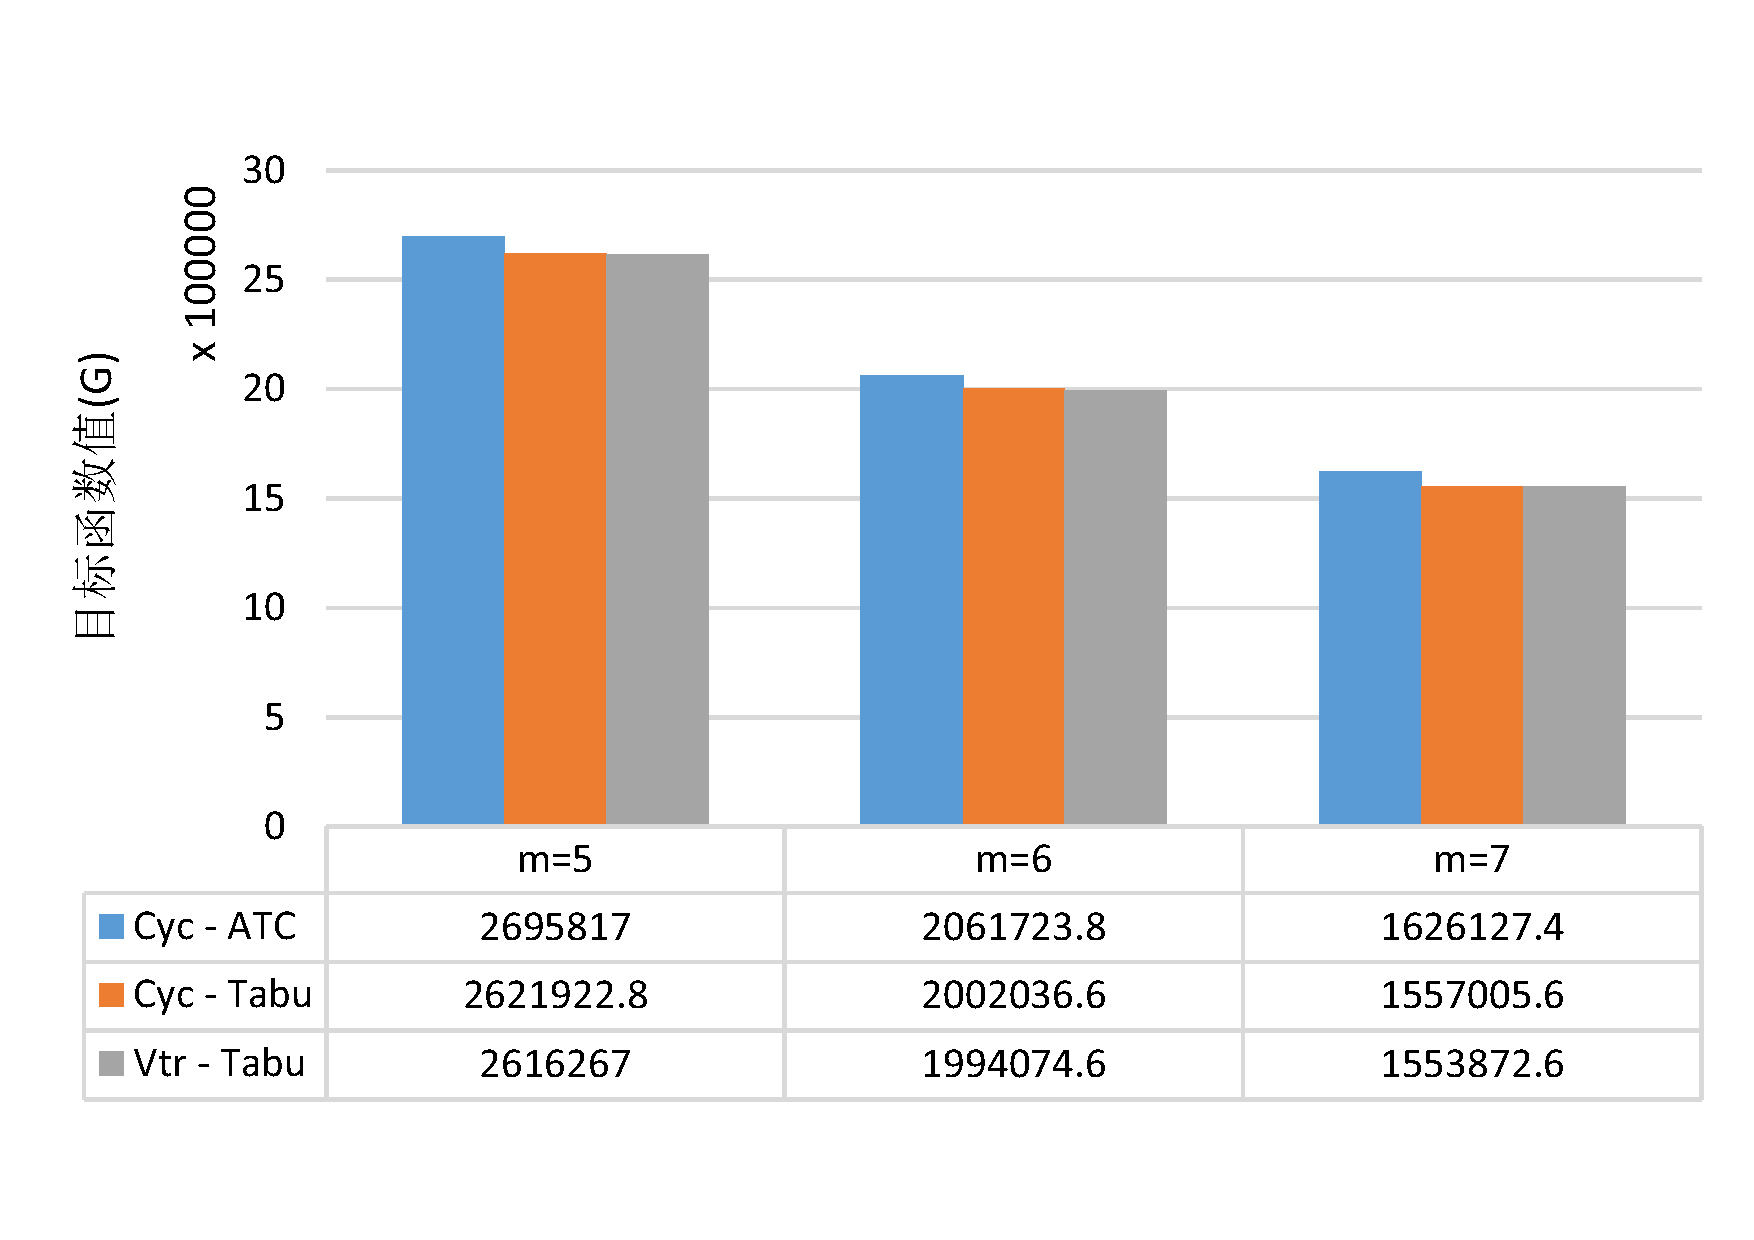
\includegraphics[height = 6cm, angle = -90]{basic_06_500}}
\subfloat[$n = 750$]{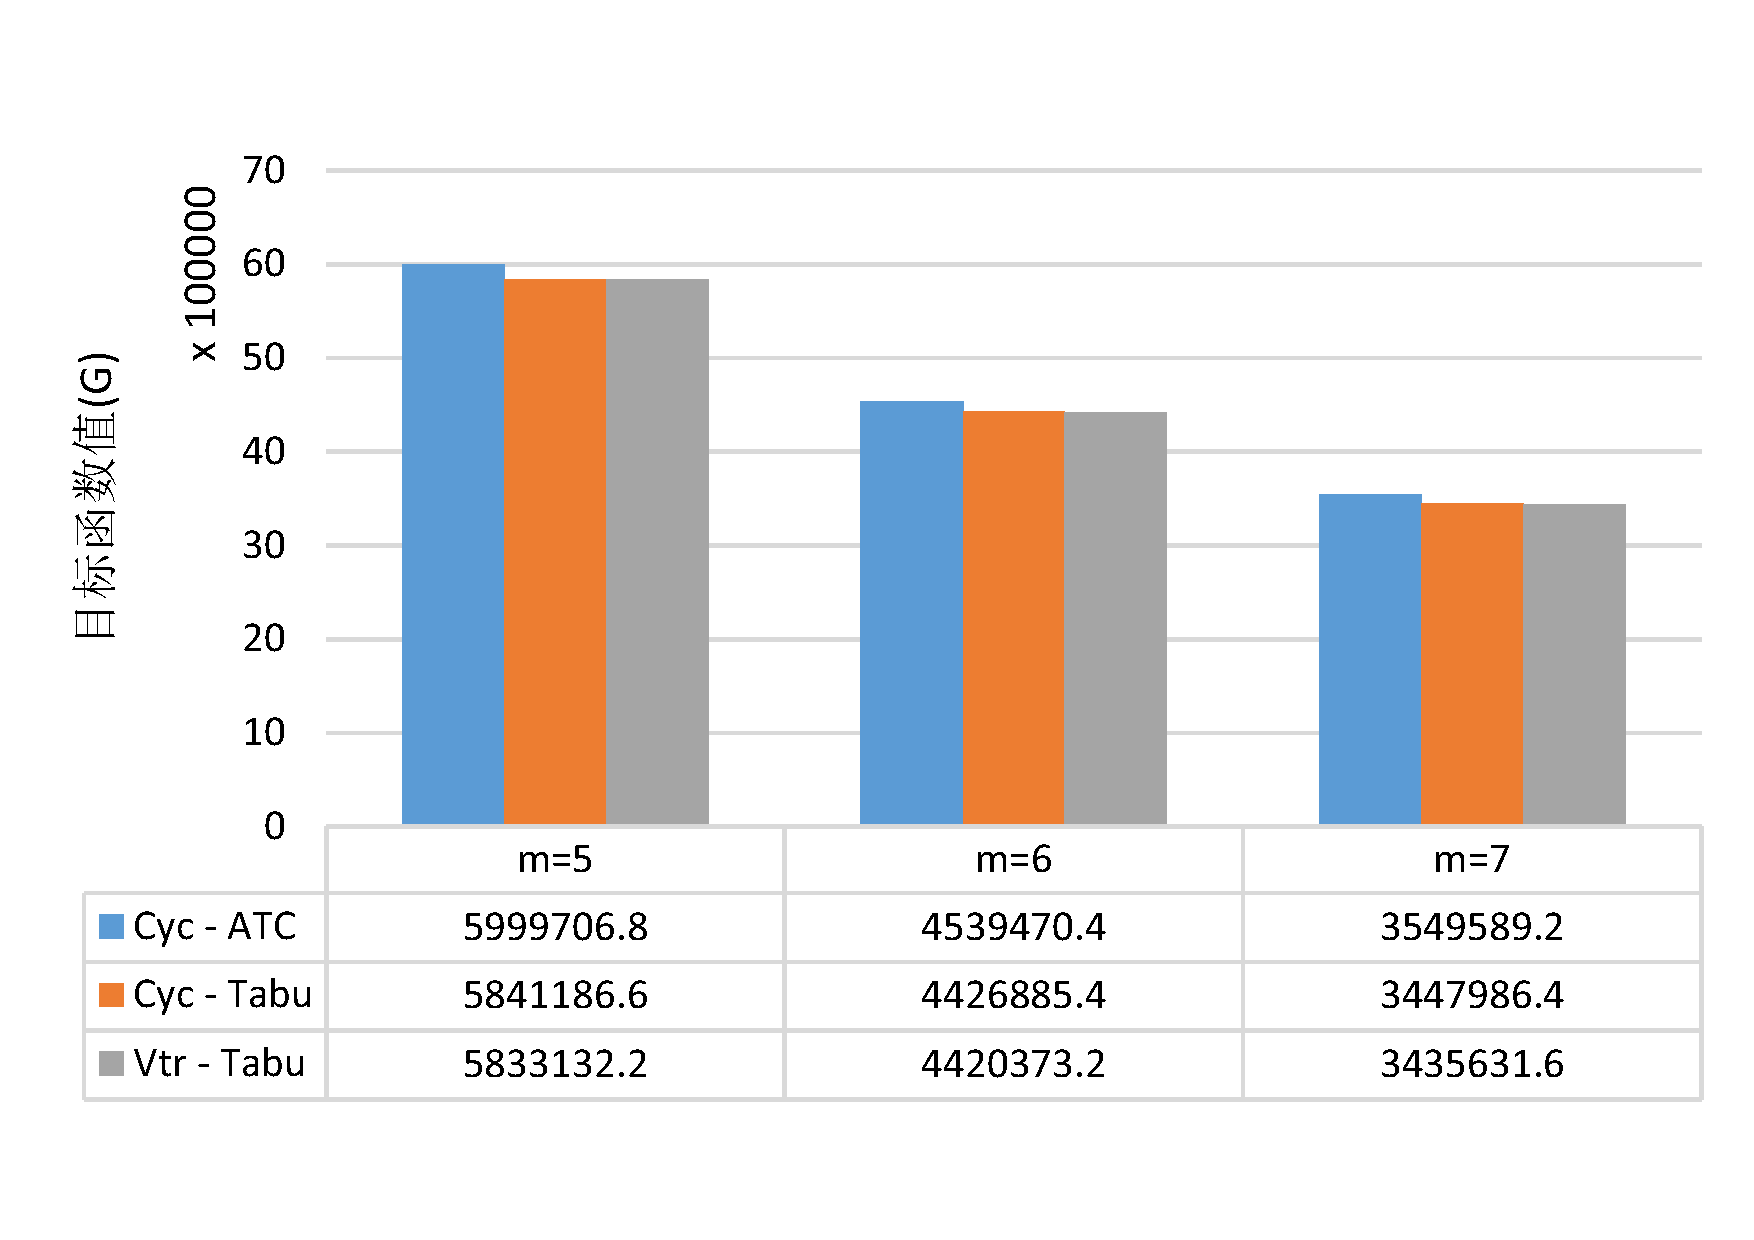
\includegraphics[height = 6cm, angle = -90]{basic_06_750}}
\subfloat[$n = 1000$]{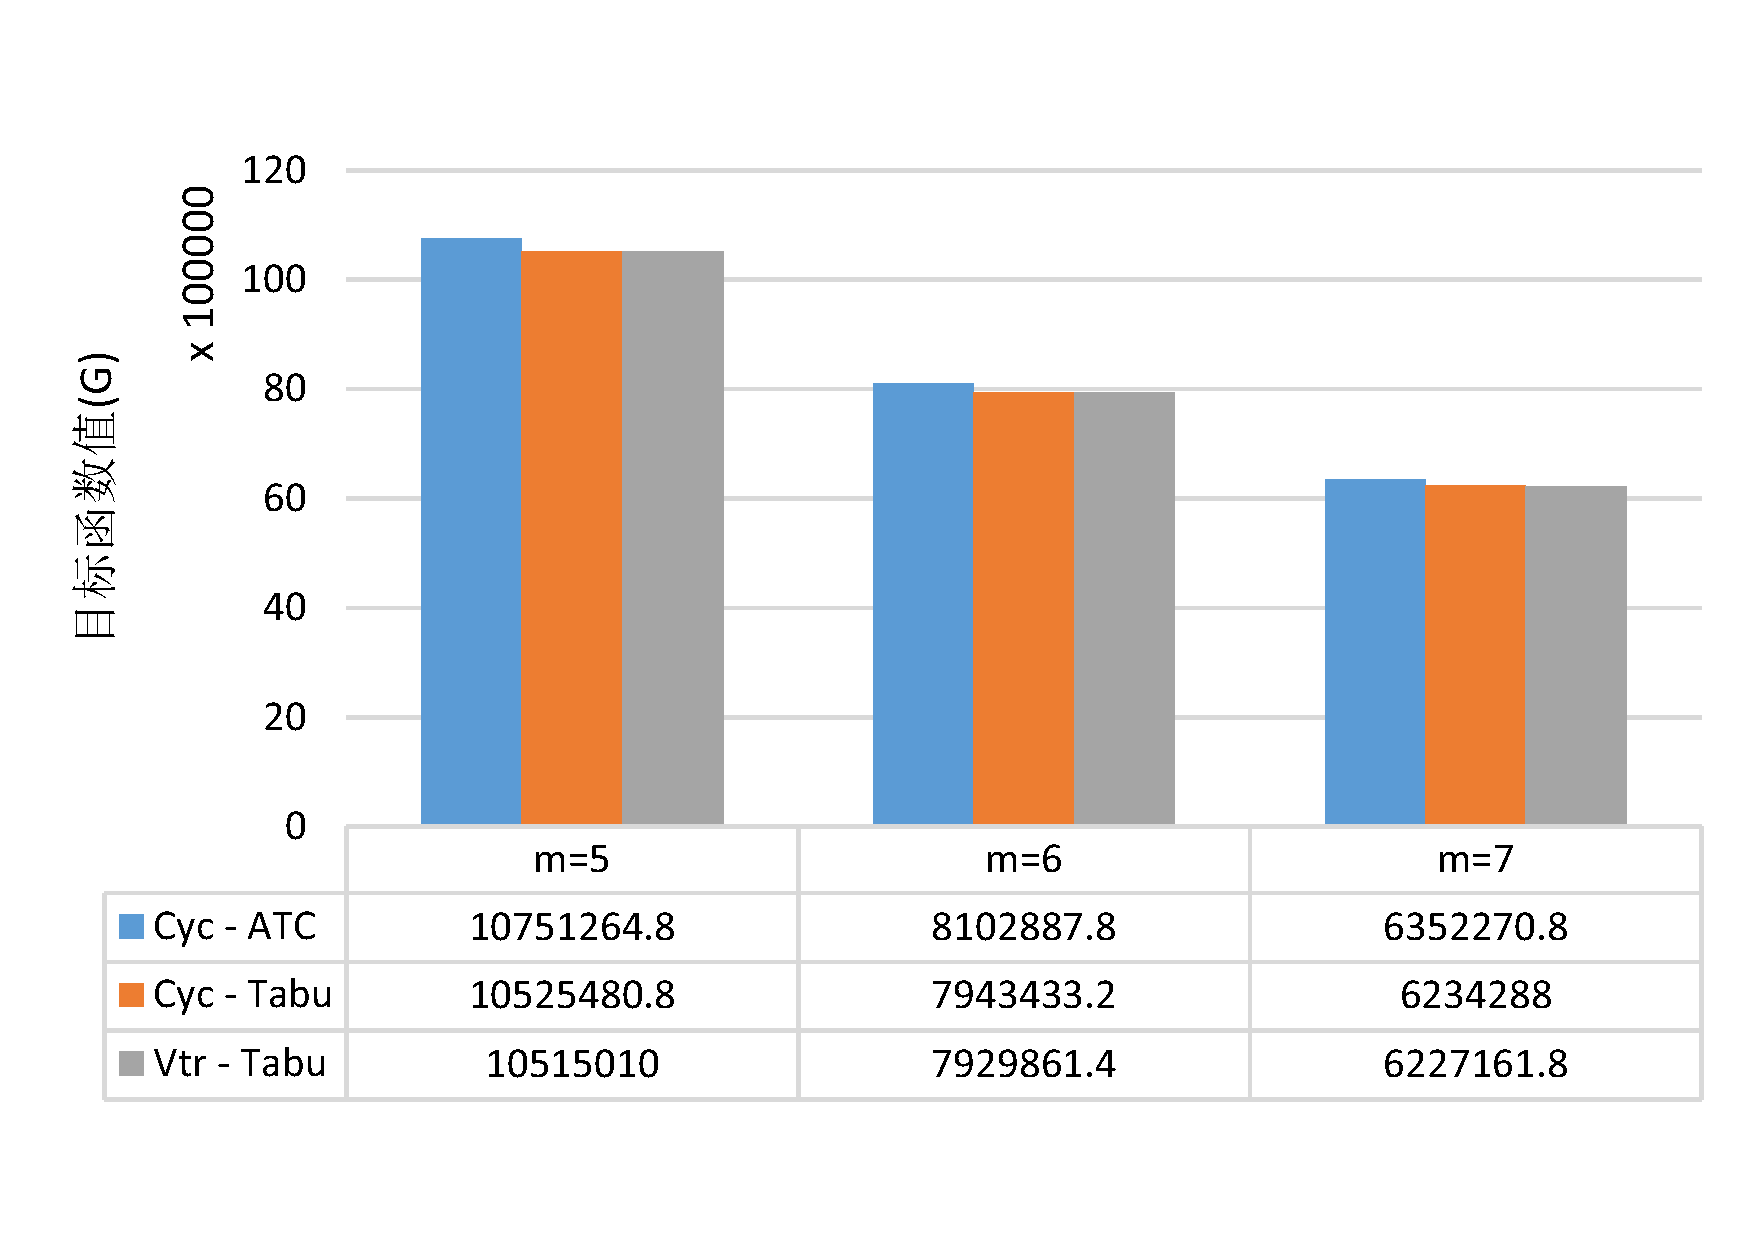
\includegraphics[height = 6cm, angle = -90]{basic_06_1000}}
\caption{\label{fig:result3}模型$1$的Cyc -- ATC、Cyc -- Tabu、Vtr -- Tabu 算法求解目标函数值比较$(\lambda_1 = 0.6)$}
\end{sidewaysfigure}

\begin{sidewaysfigure}
\centering
\subfloat[$n = 20$]{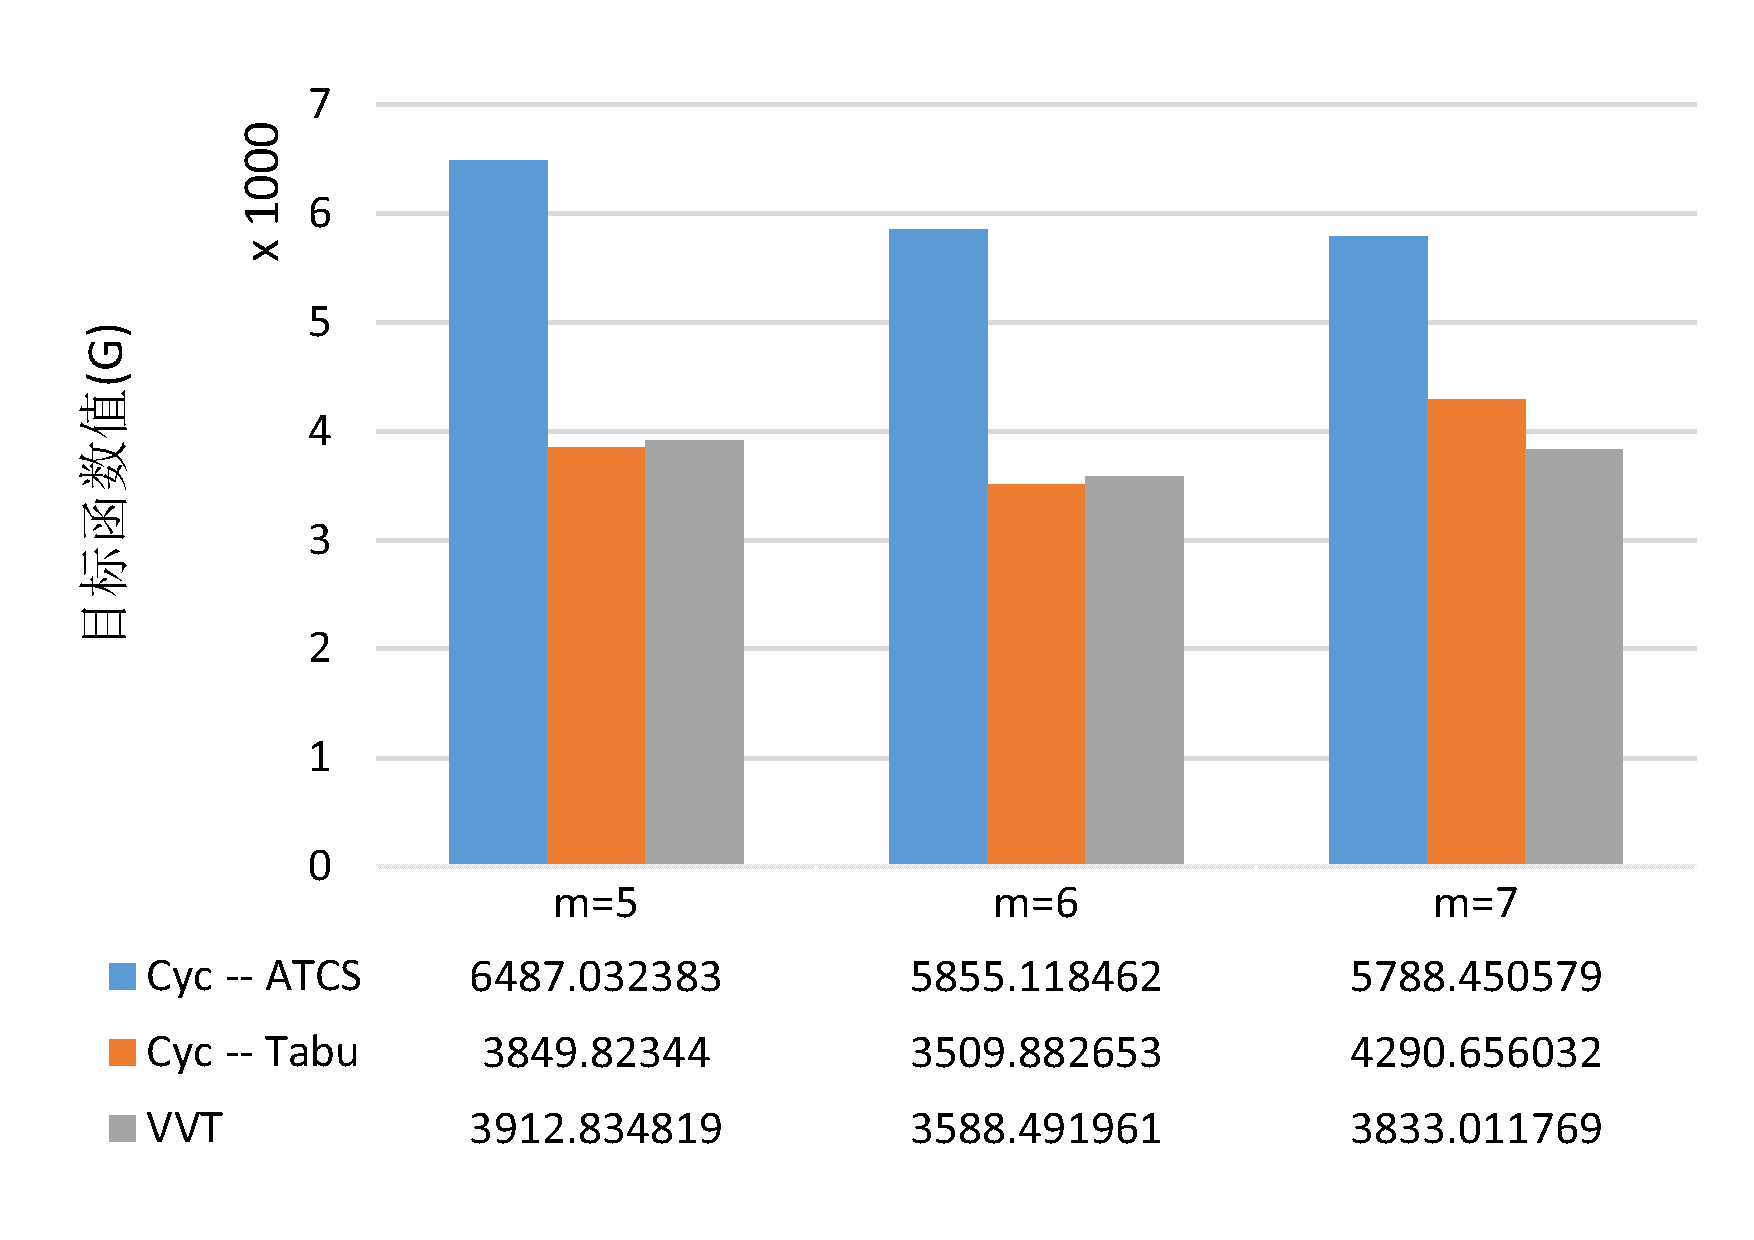
\includegraphics[height = 6cm, angle = -90]{continue_04_20}}
\subfloat[$n = 30$]{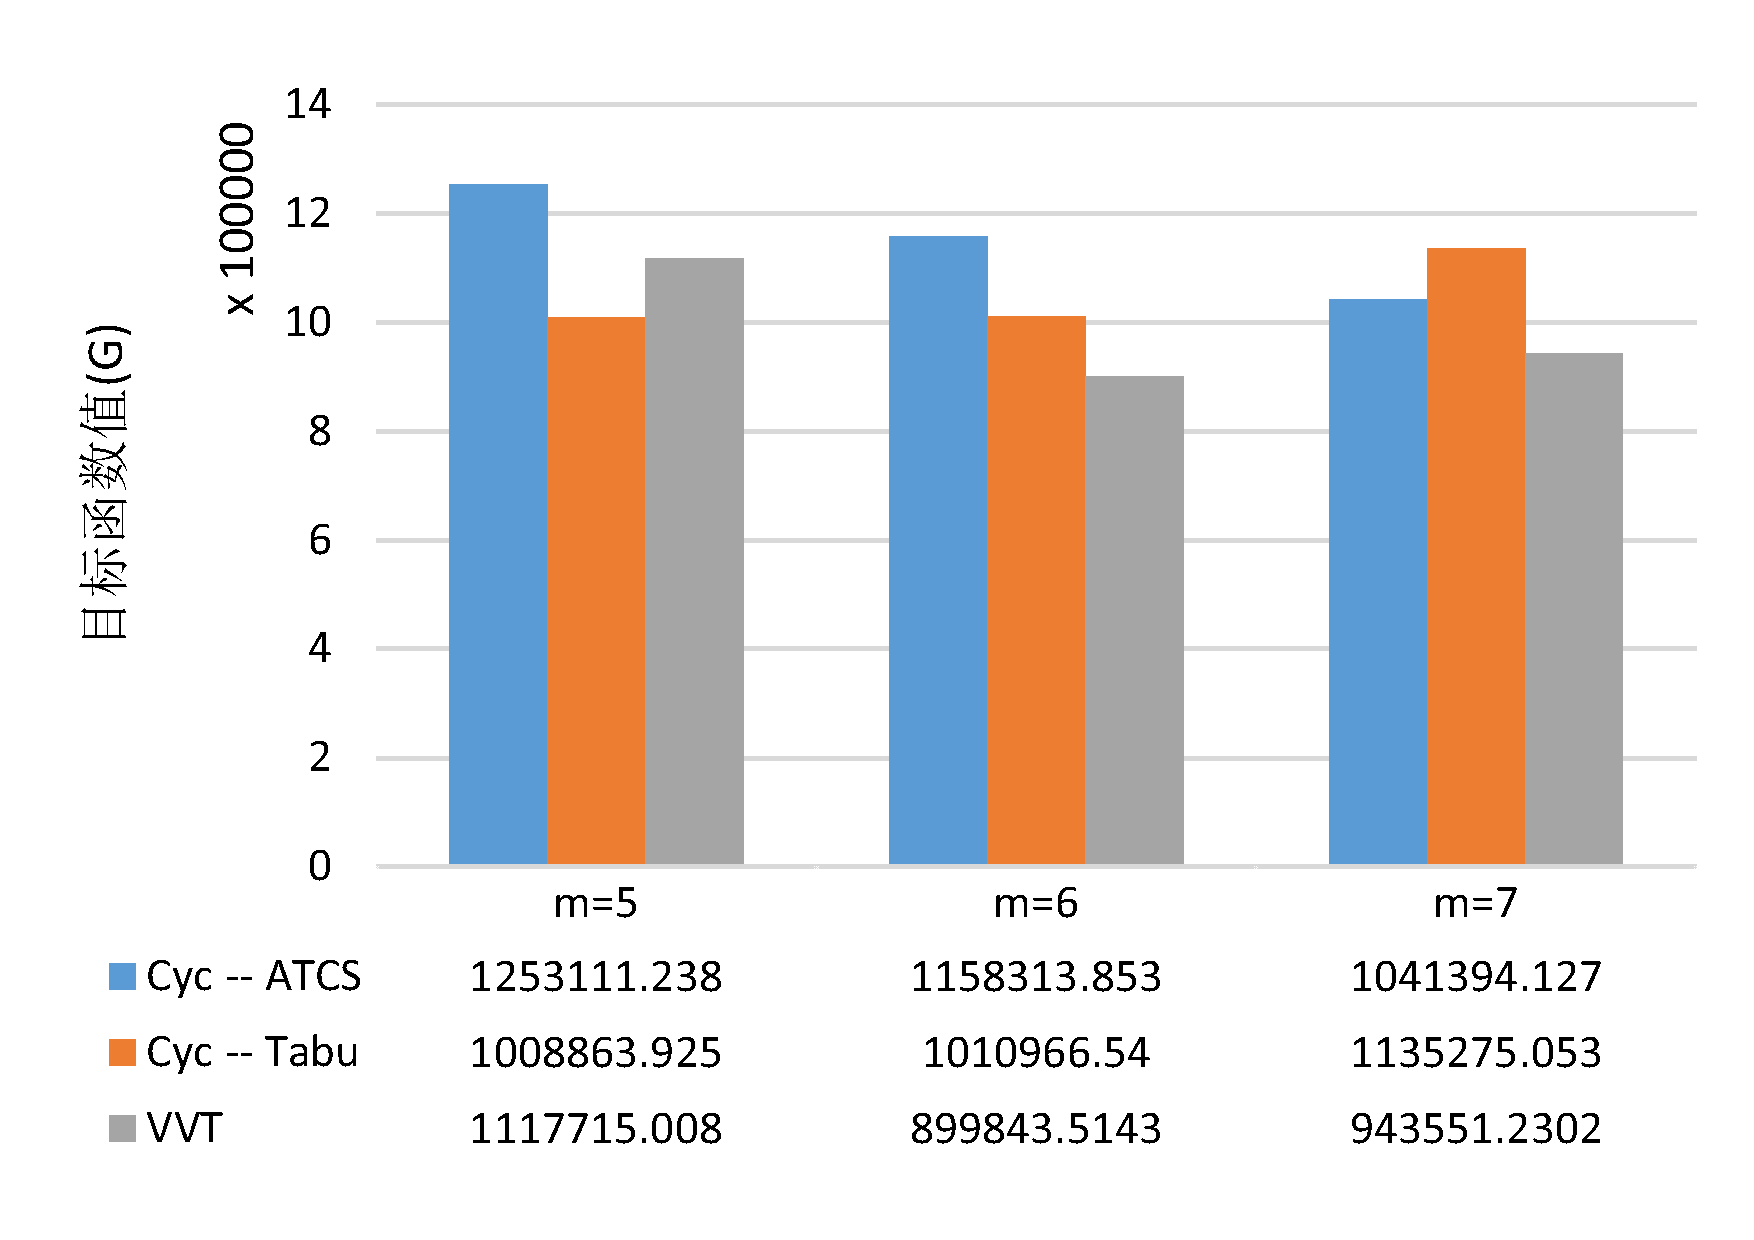
\includegraphics[height = 6cm, angle = -90]{continue_04_300}}
\subfloat[$n = 50$]{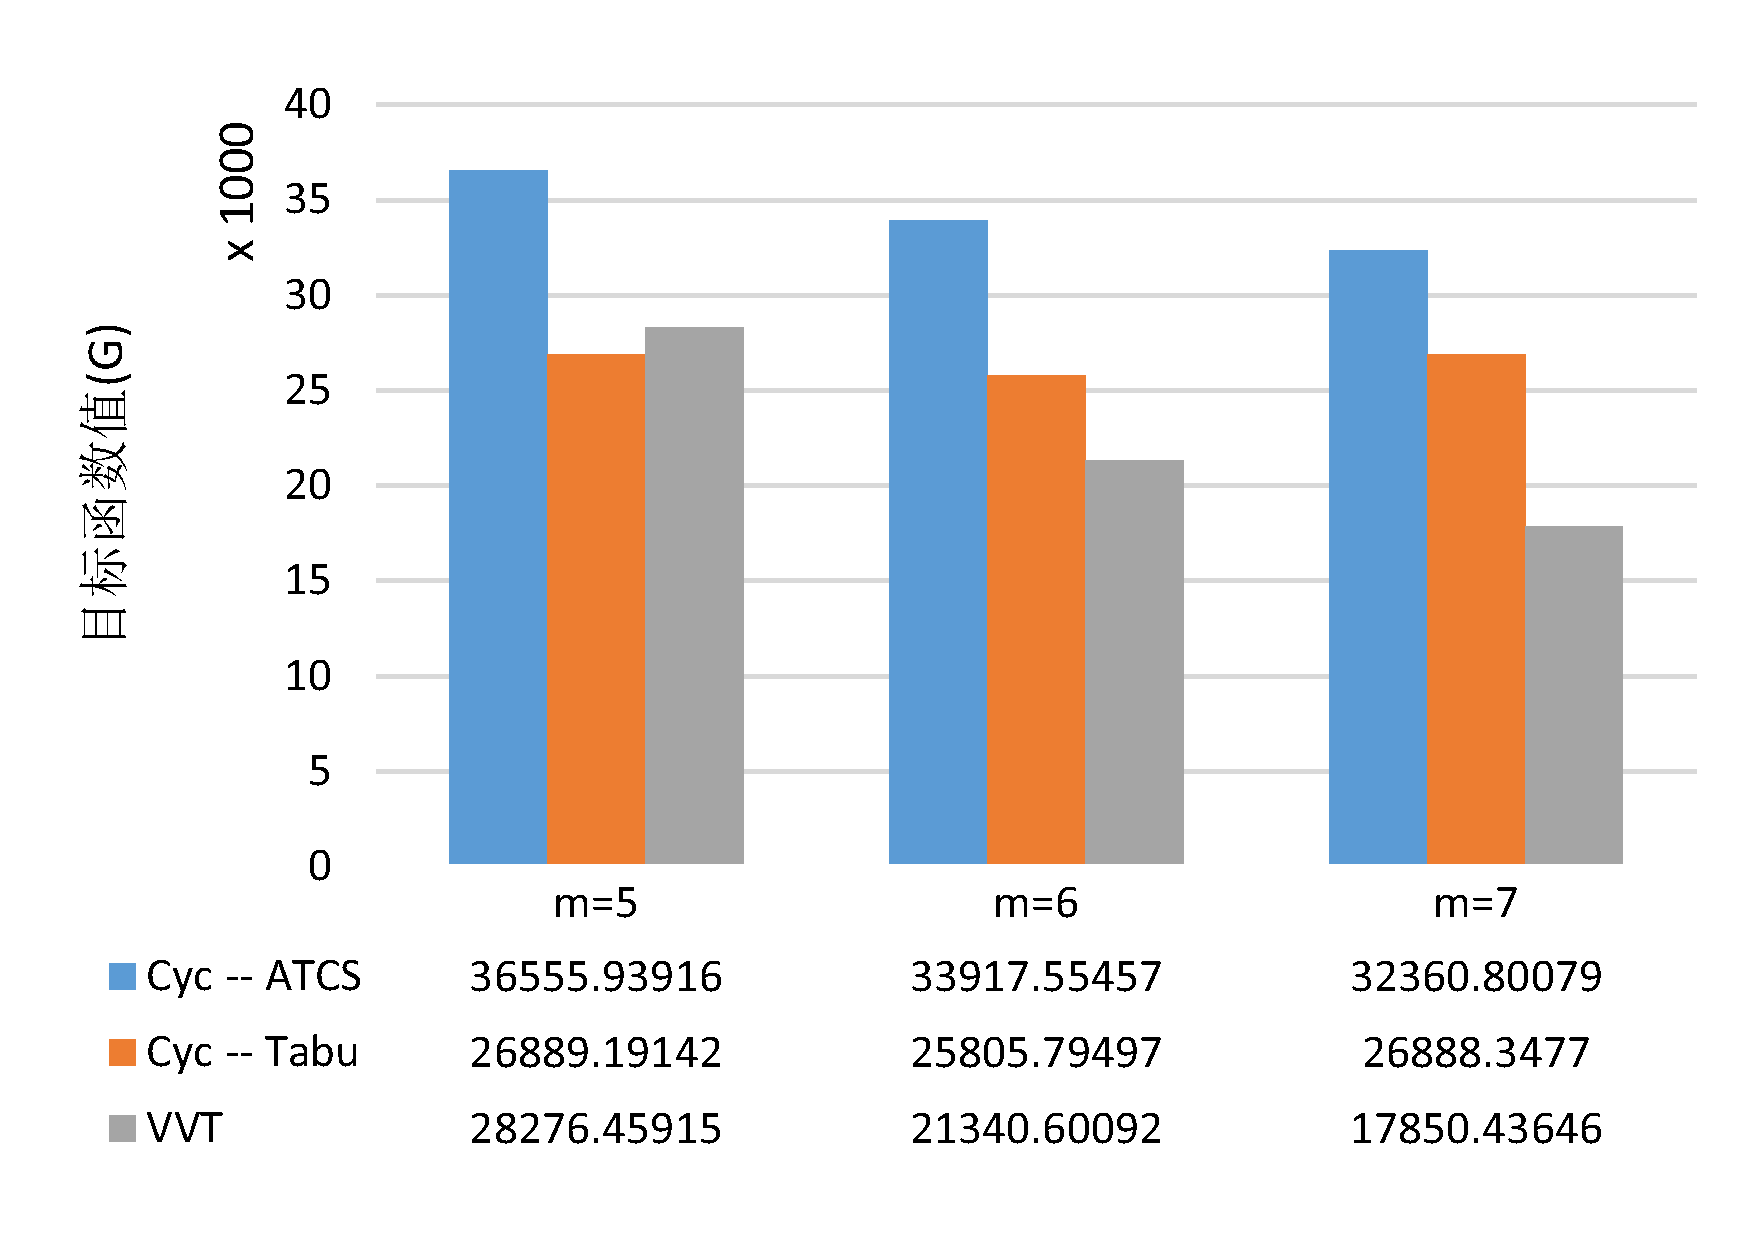
\includegraphics[height = 6cm, angle = -90]{continue_04_50}}
\subfloat[$n = 70$]{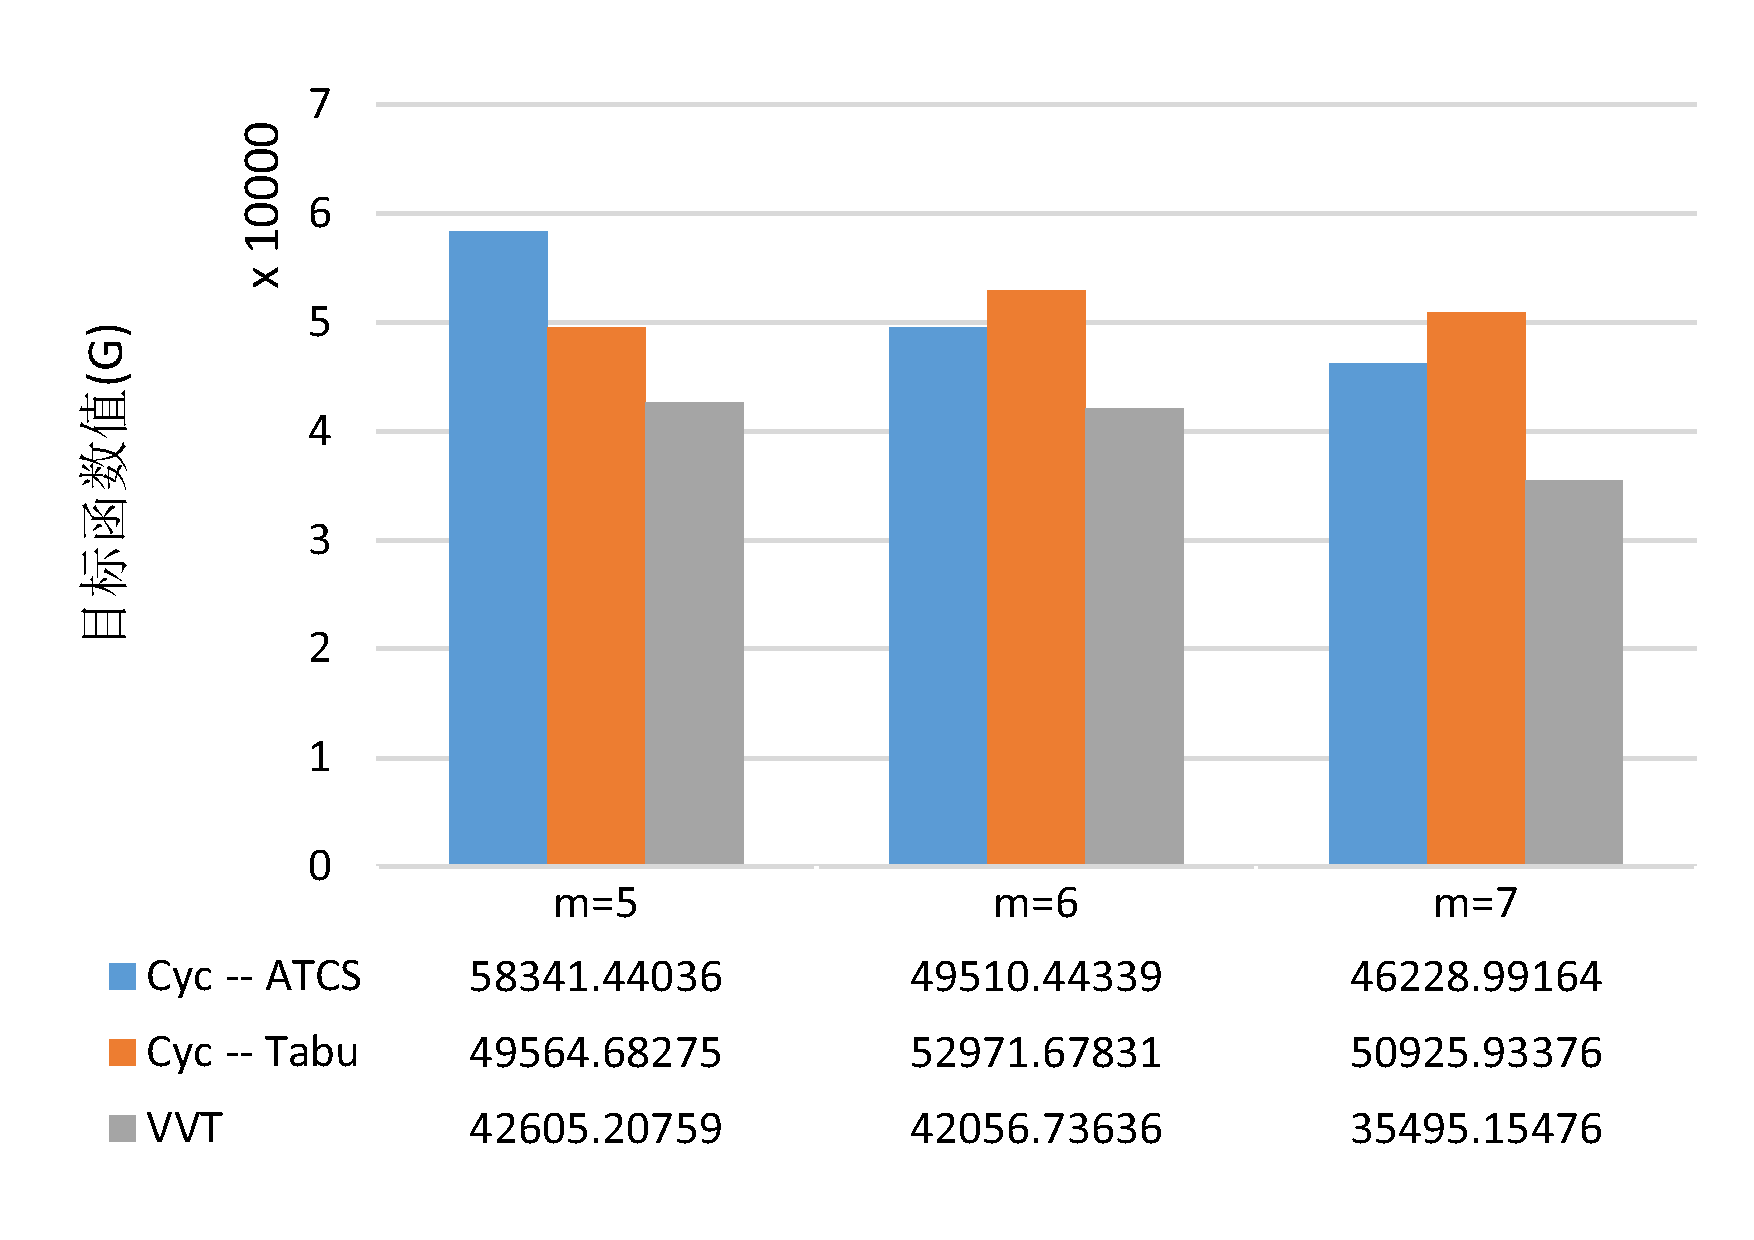
\includegraphics[height = 6cm, angle = -90]{continue_04_70}}\\
\subfloat[$n = 100$]{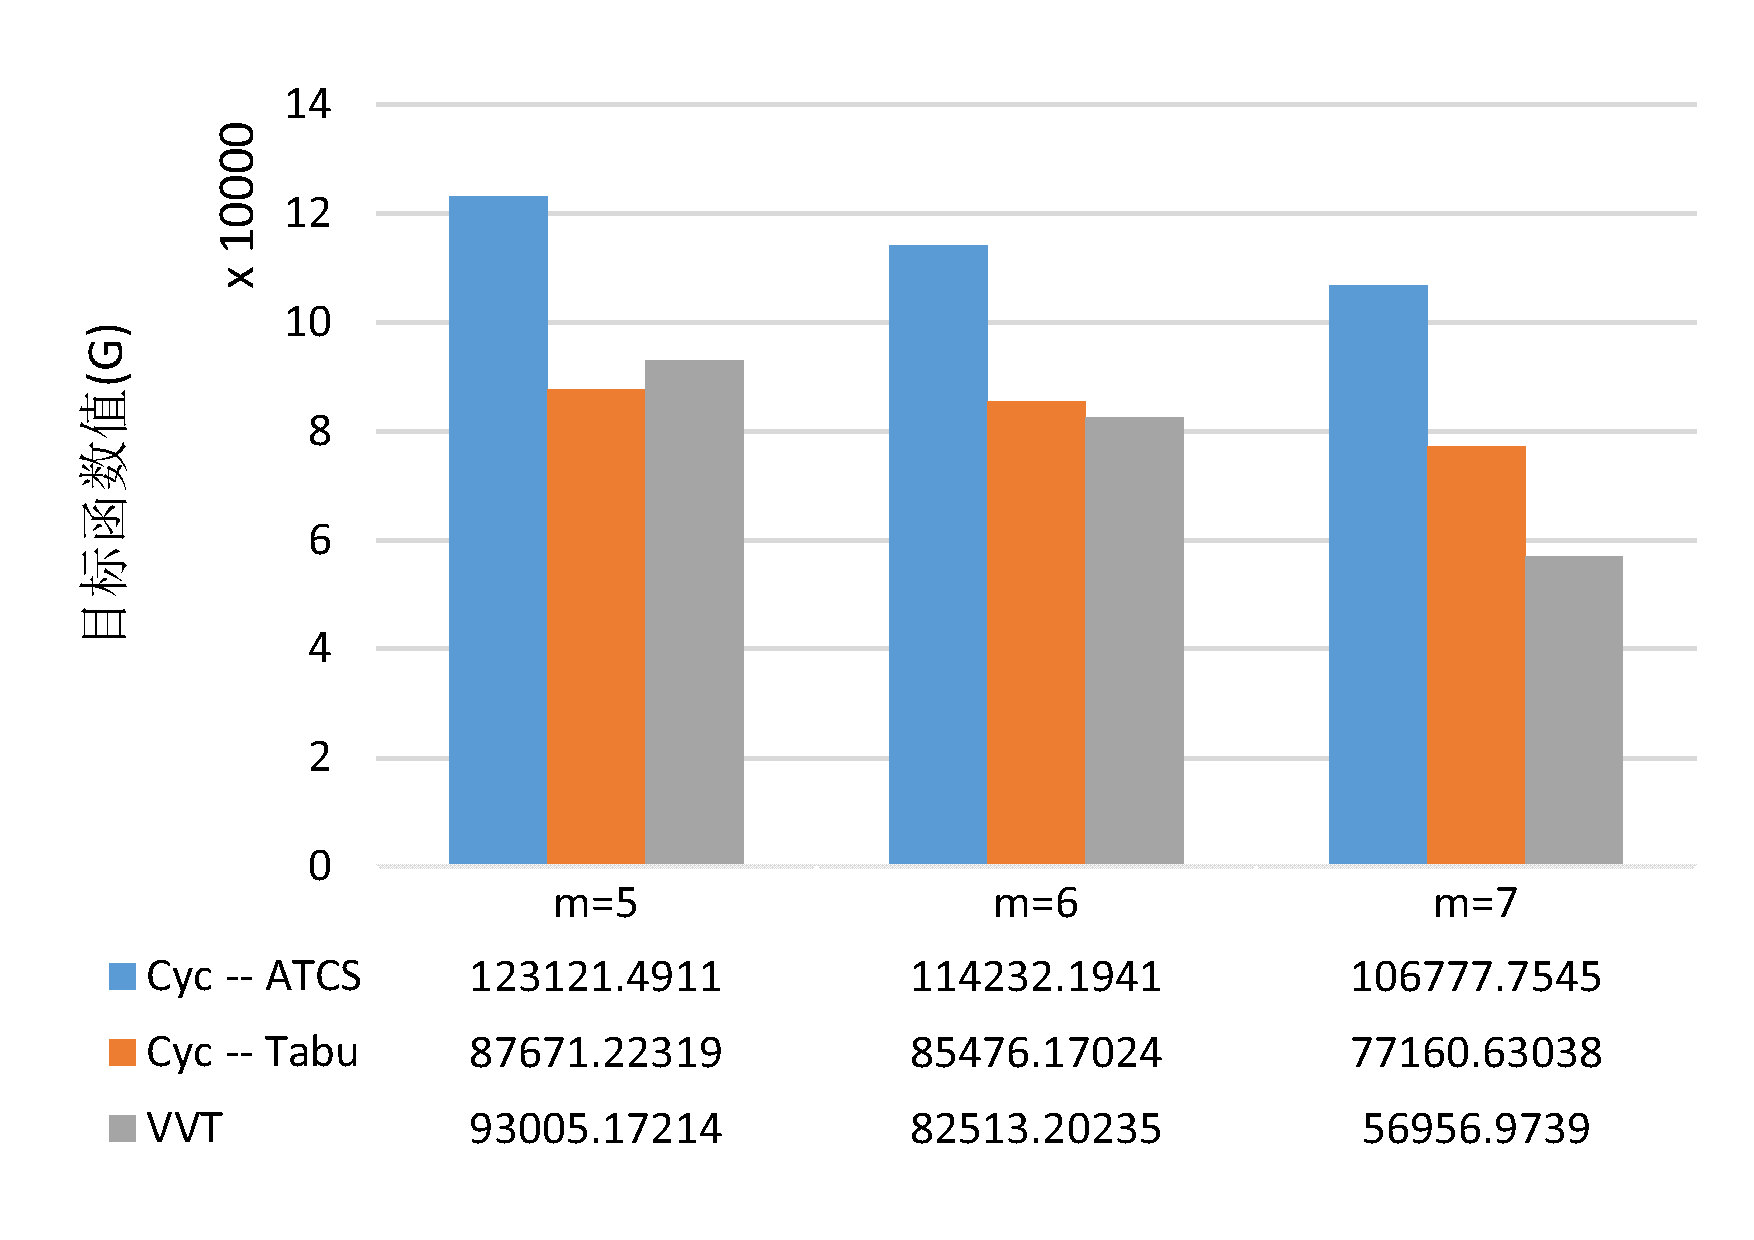
\includegraphics[height = 6cm, angle = -90]{continue_04_100}}
\subfloat[$n = 150$]{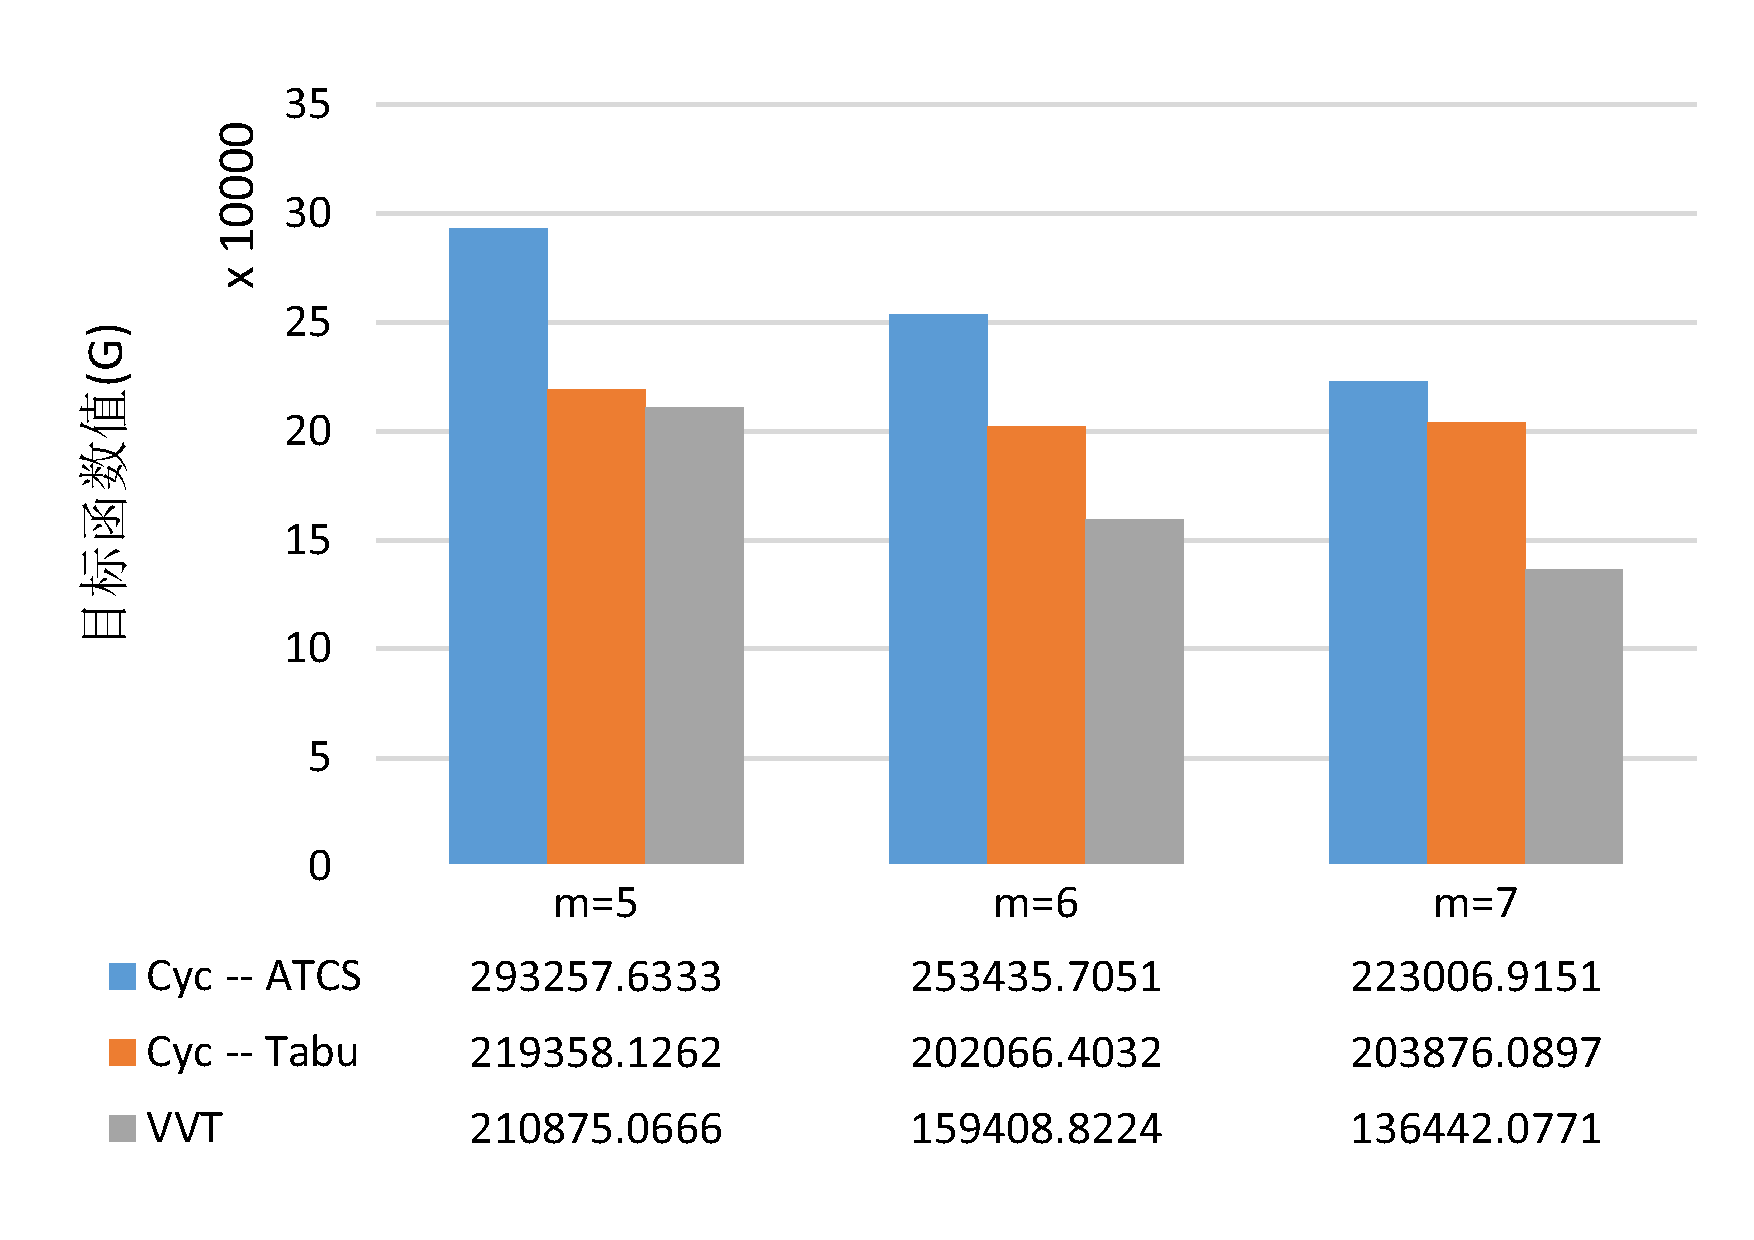
\includegraphics[height = 6cm, angle = -90]{continue_04_150}}
\subfloat[$n = 200$]{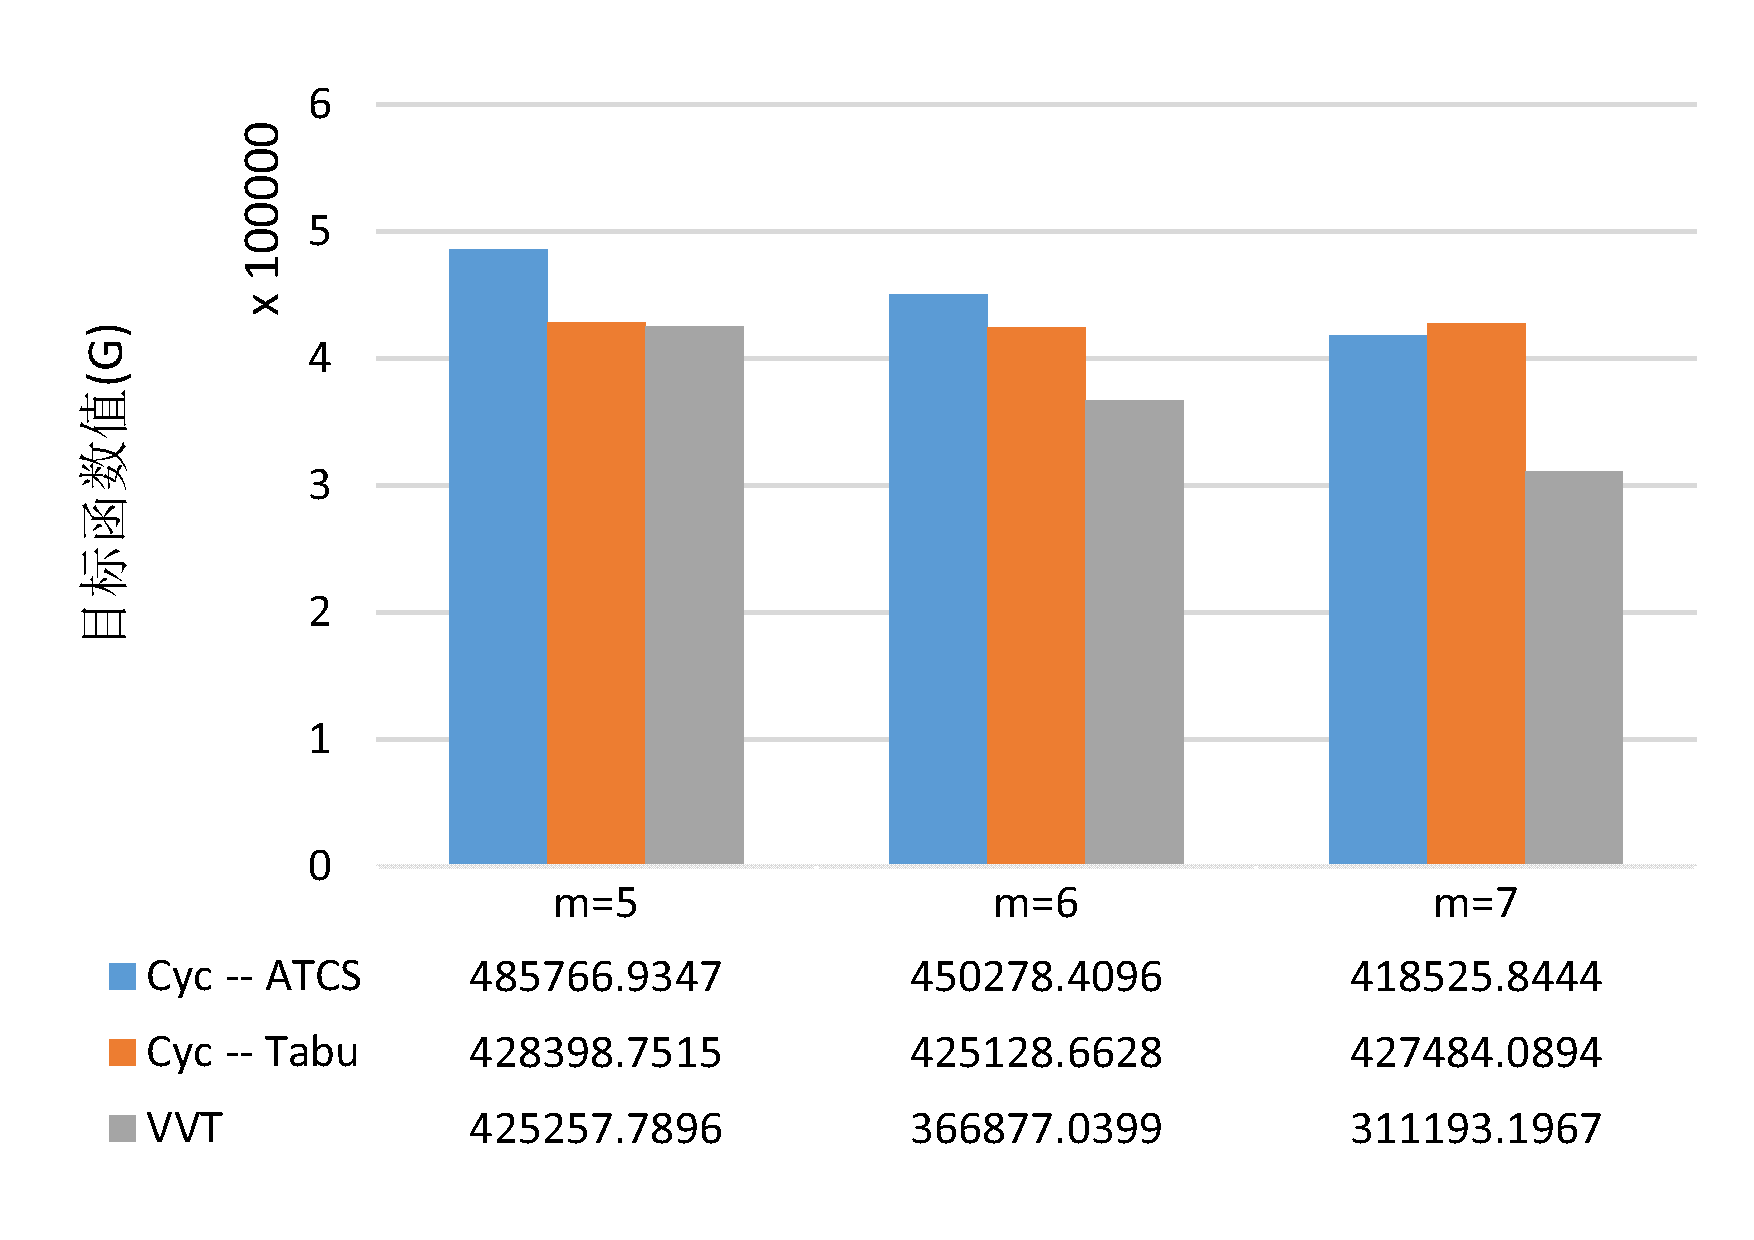
\includegraphics[height = 6cm, angle = -90]{continue_04_200}}
\subfloat[$n = 300$]{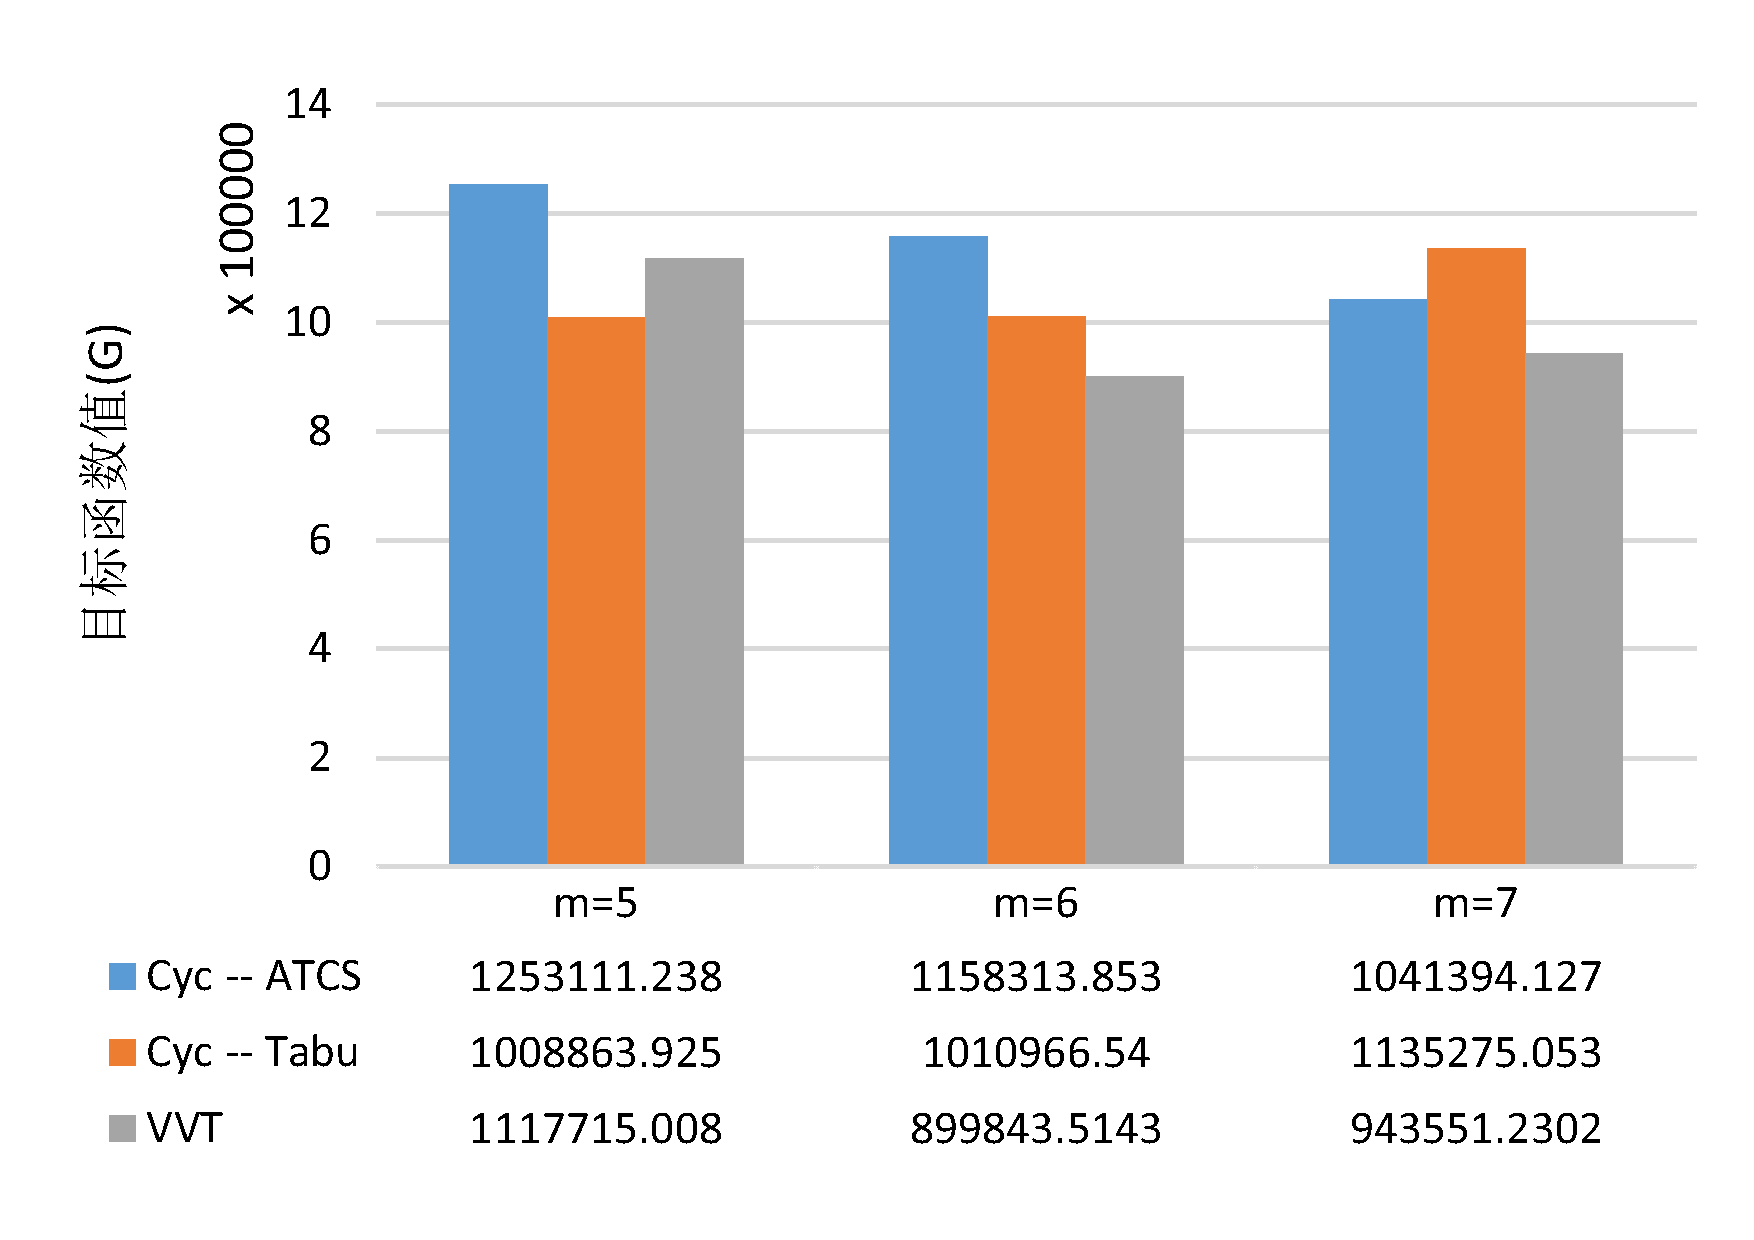
\includegraphics[height = 6cm, angle = -90]{continue_04_300}}\\
\subfloat[$n = 500$]{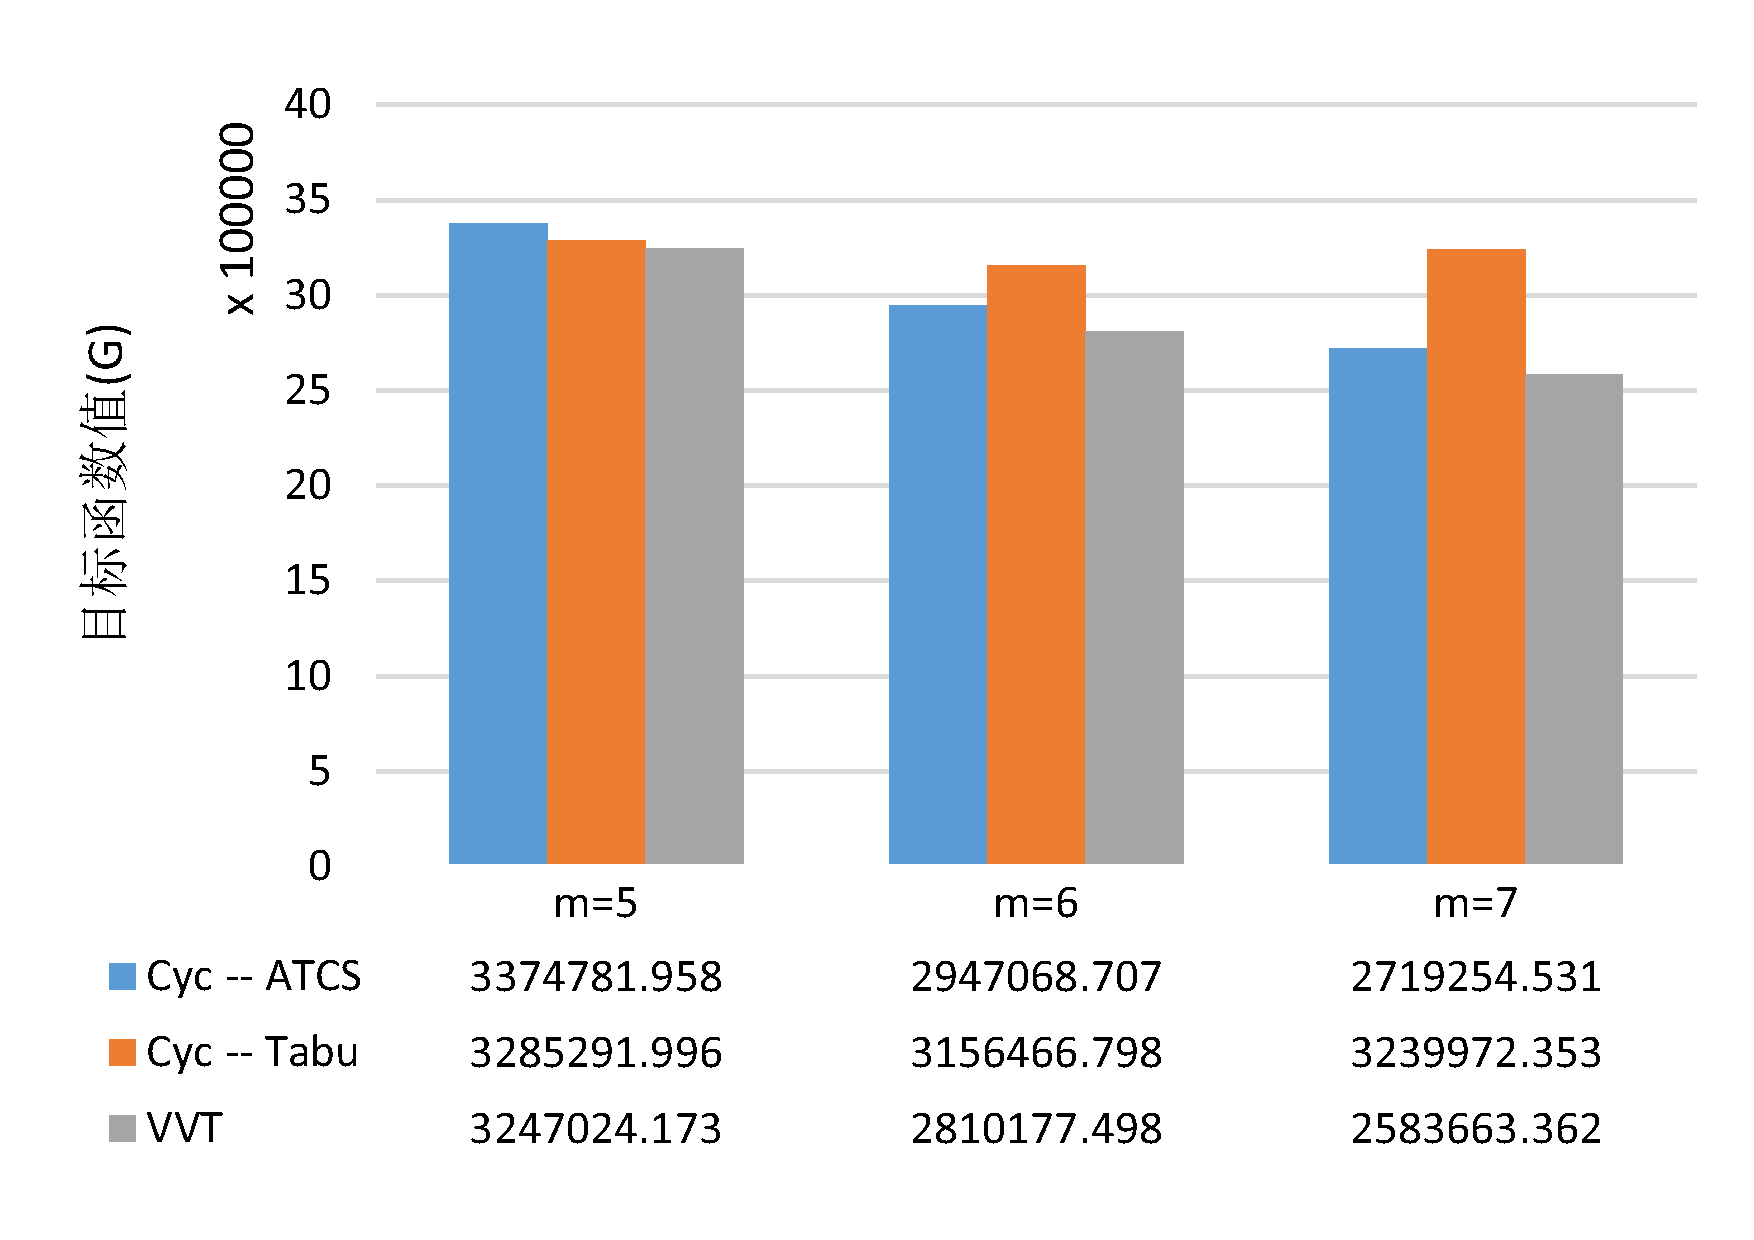
\includegraphics[height = 6cm, angle = -90]{continue_04_500}}
\subfloat[$n = 750$]{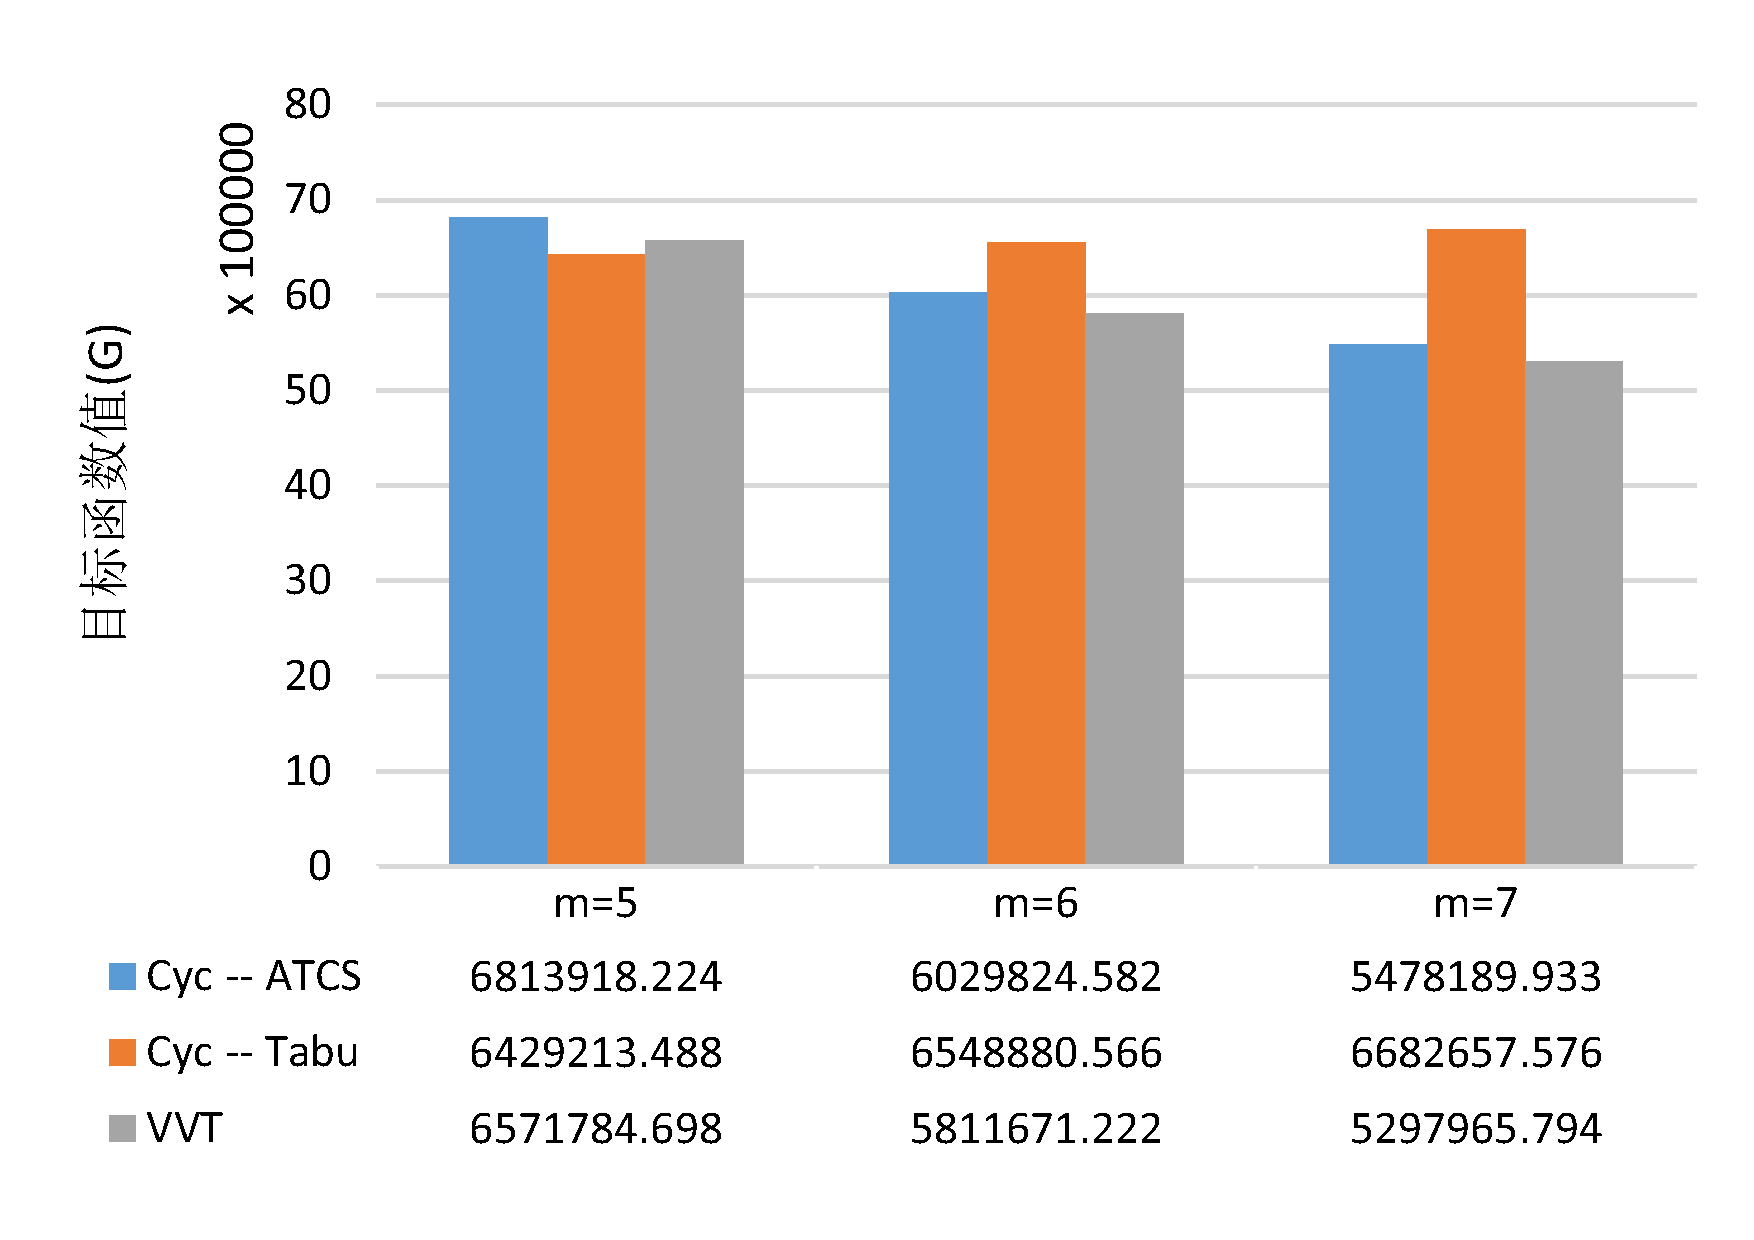
\includegraphics[height = 6cm, angle = -90]{continue_04_750}}
\subfloat[$n = 1000$]{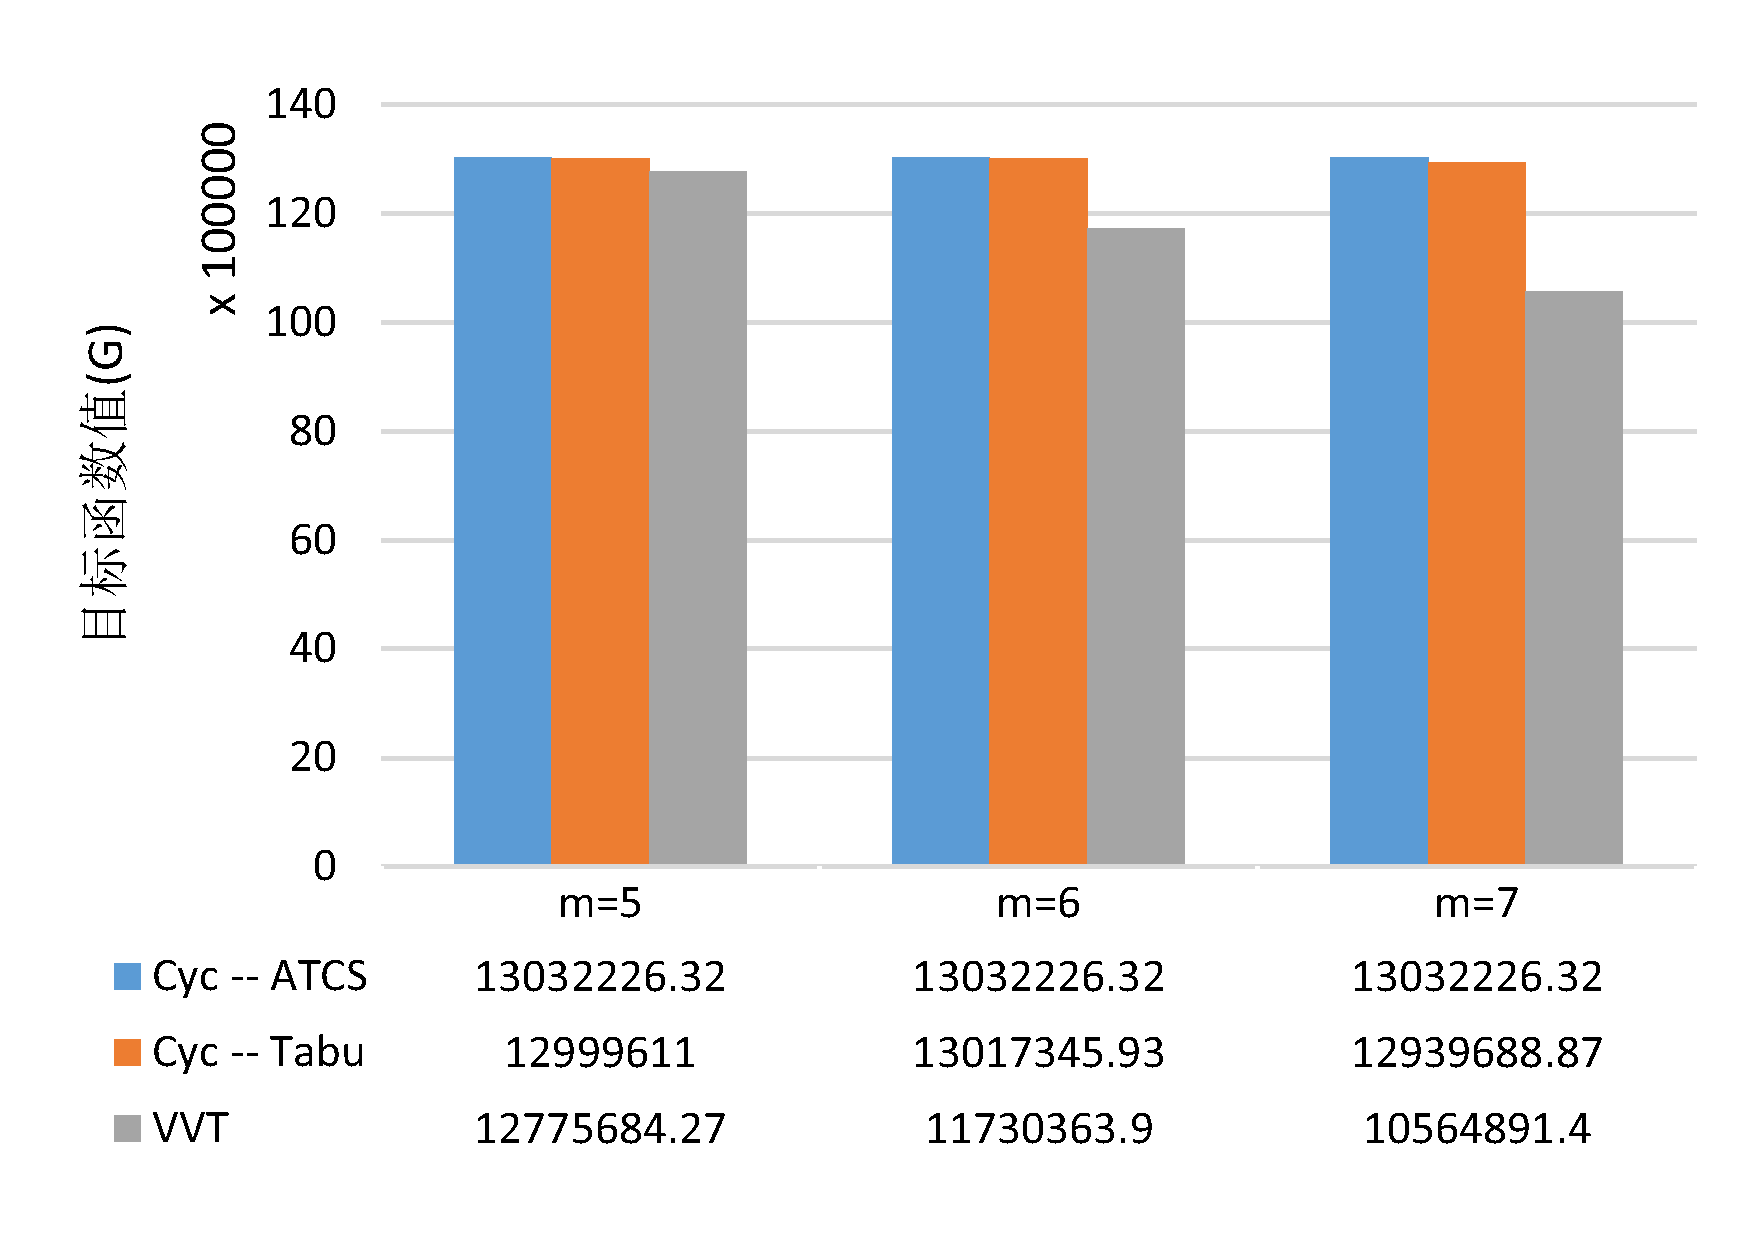
\includegraphics[height = 6cm, angle = -90]{continue_04_1000}}
\caption{\label{fig:result4}模型$2$的Cyc -- ATCS、Cyc -- Tabu、VVT 算法求解目标函数值比较$(\lambda_1 = 0.4)$}
\end{sidewaysfigure}

\begin{sidewaysfigure}
\centering
\subfloat[$n = 20$]{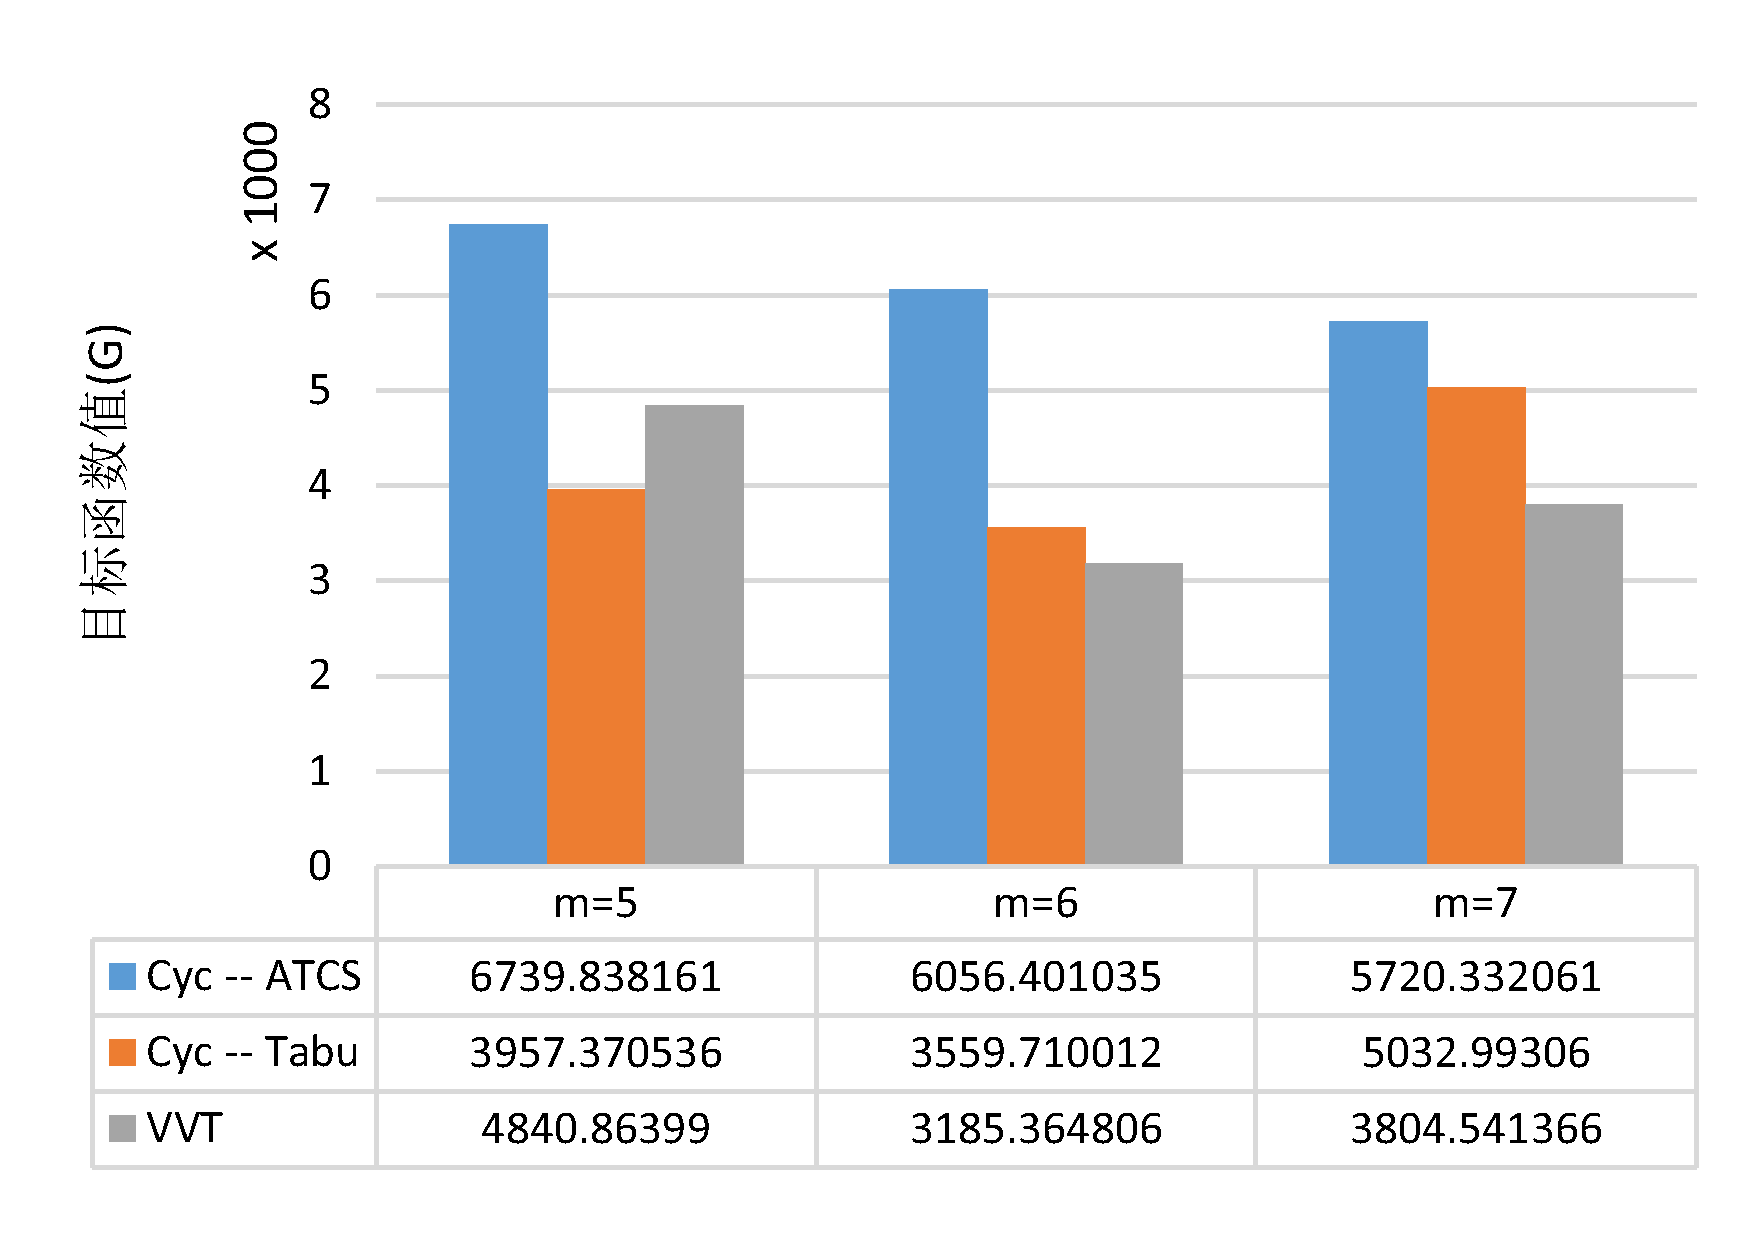
\includegraphics[height = 6cm, angle = -90]{continue_05_20}}
\subfloat[$n = 30$]{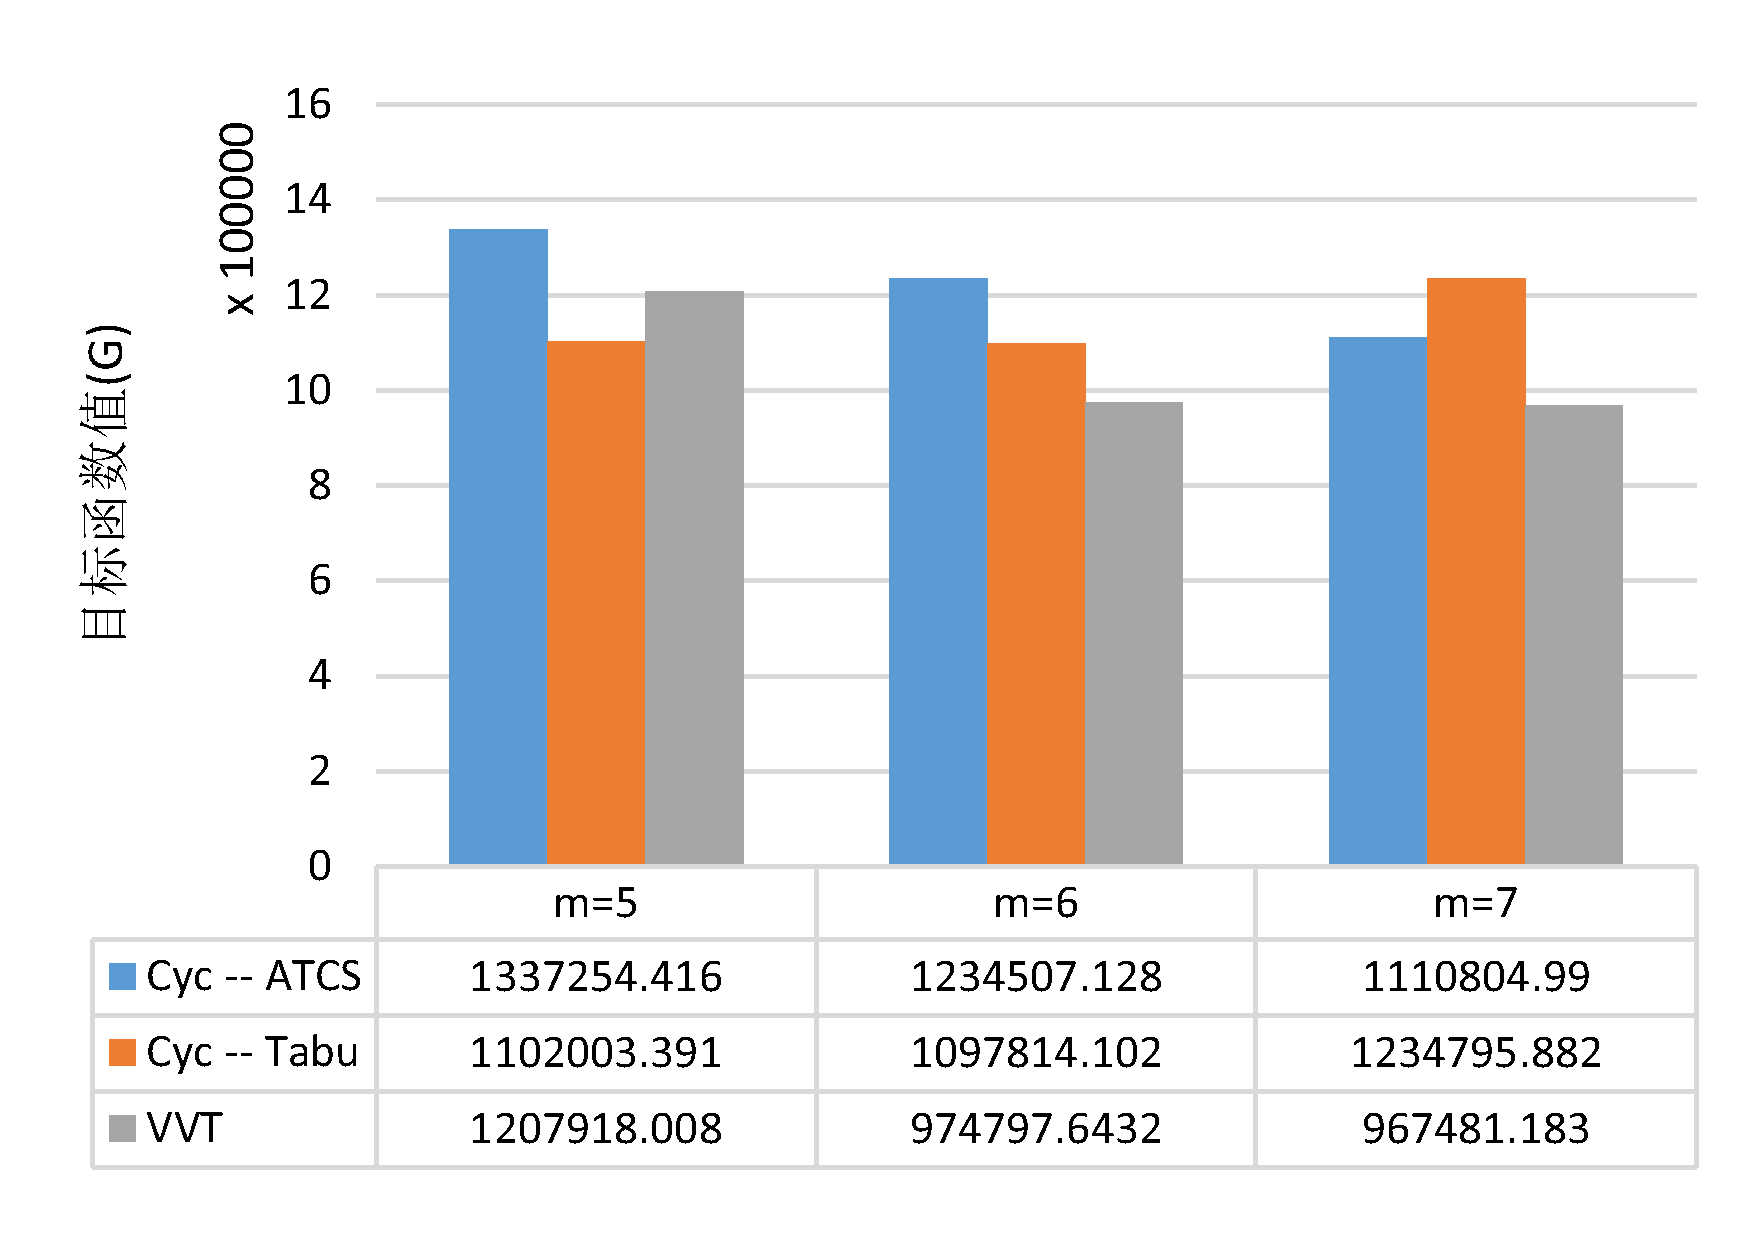
\includegraphics[height = 6cm, angle = -90]{continue_05_300}}
\subfloat[$n = 50$]{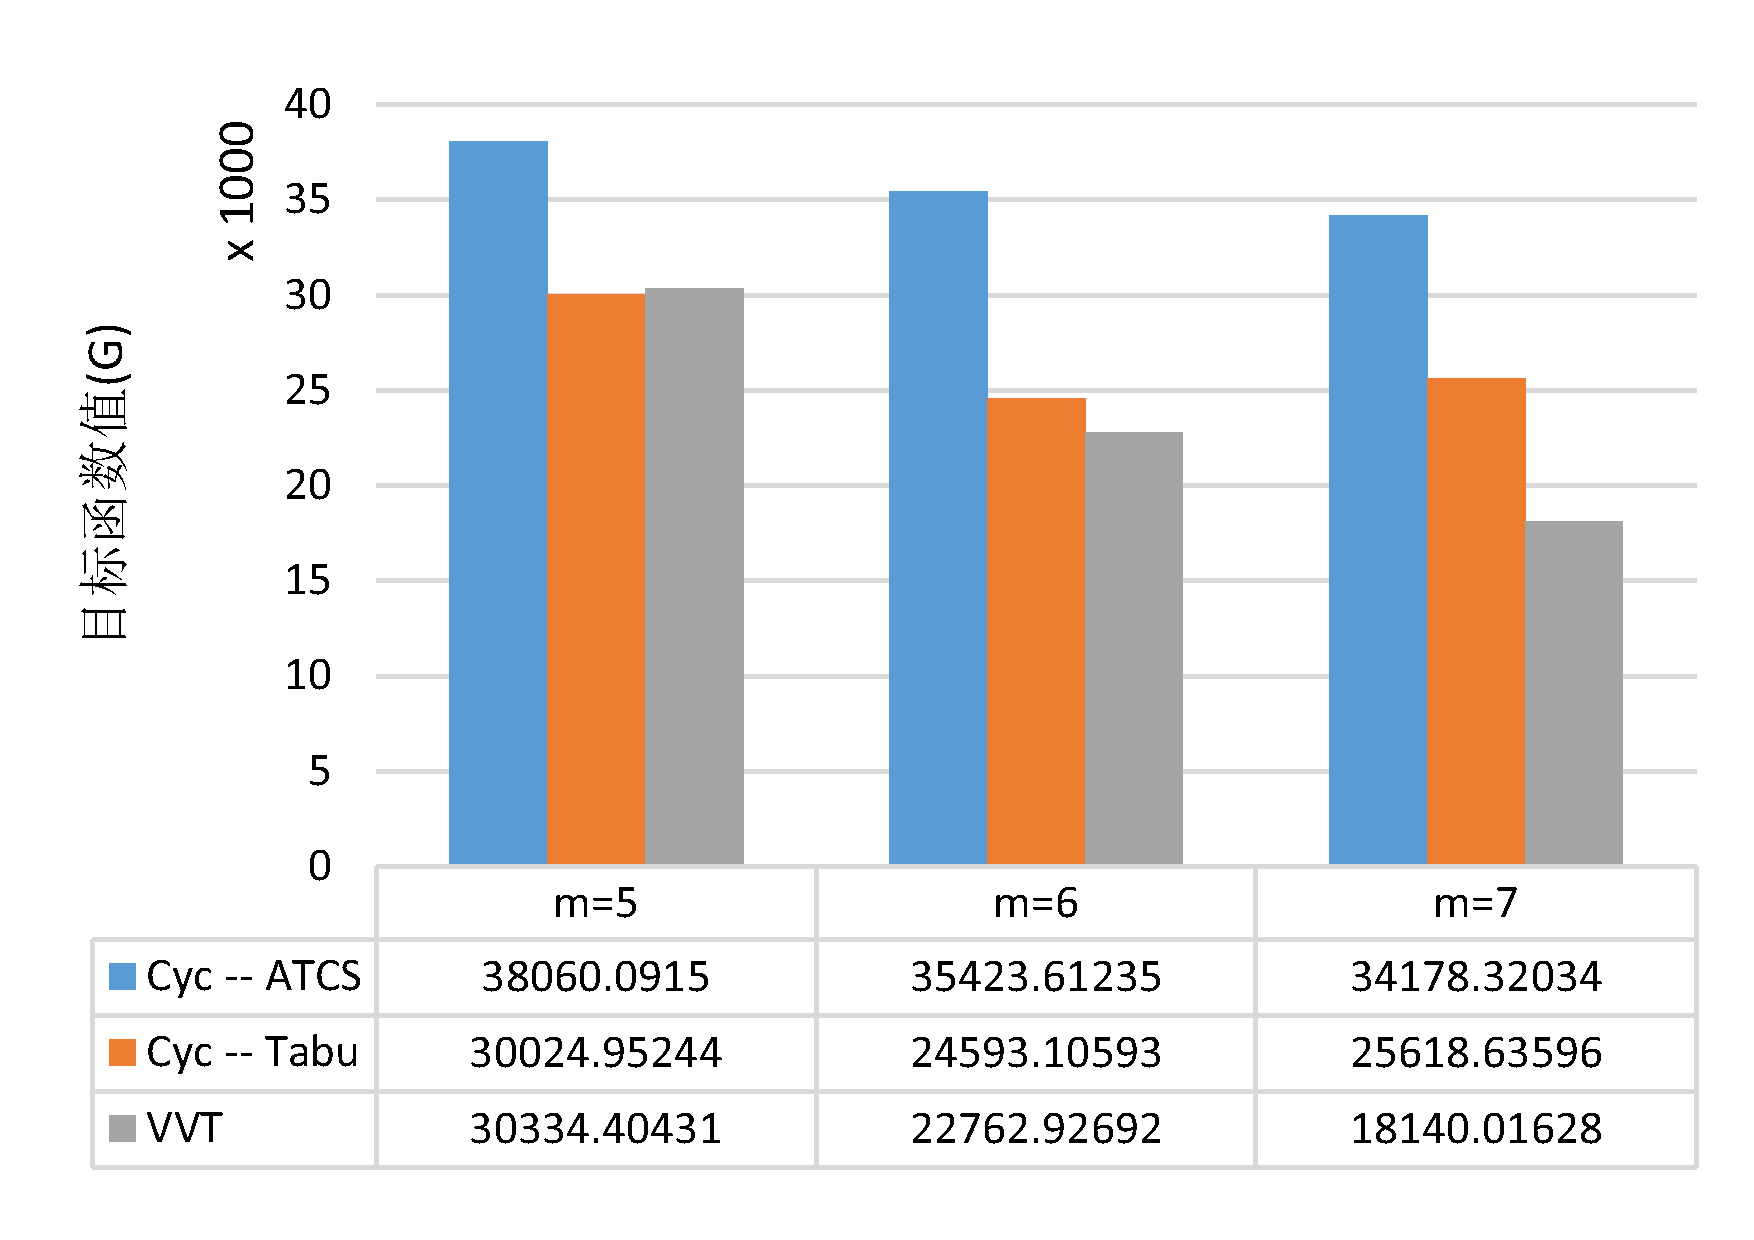
\includegraphics[height = 6cm, angle = -90]{continue_05_50}}
\subfloat[$n = 70$]{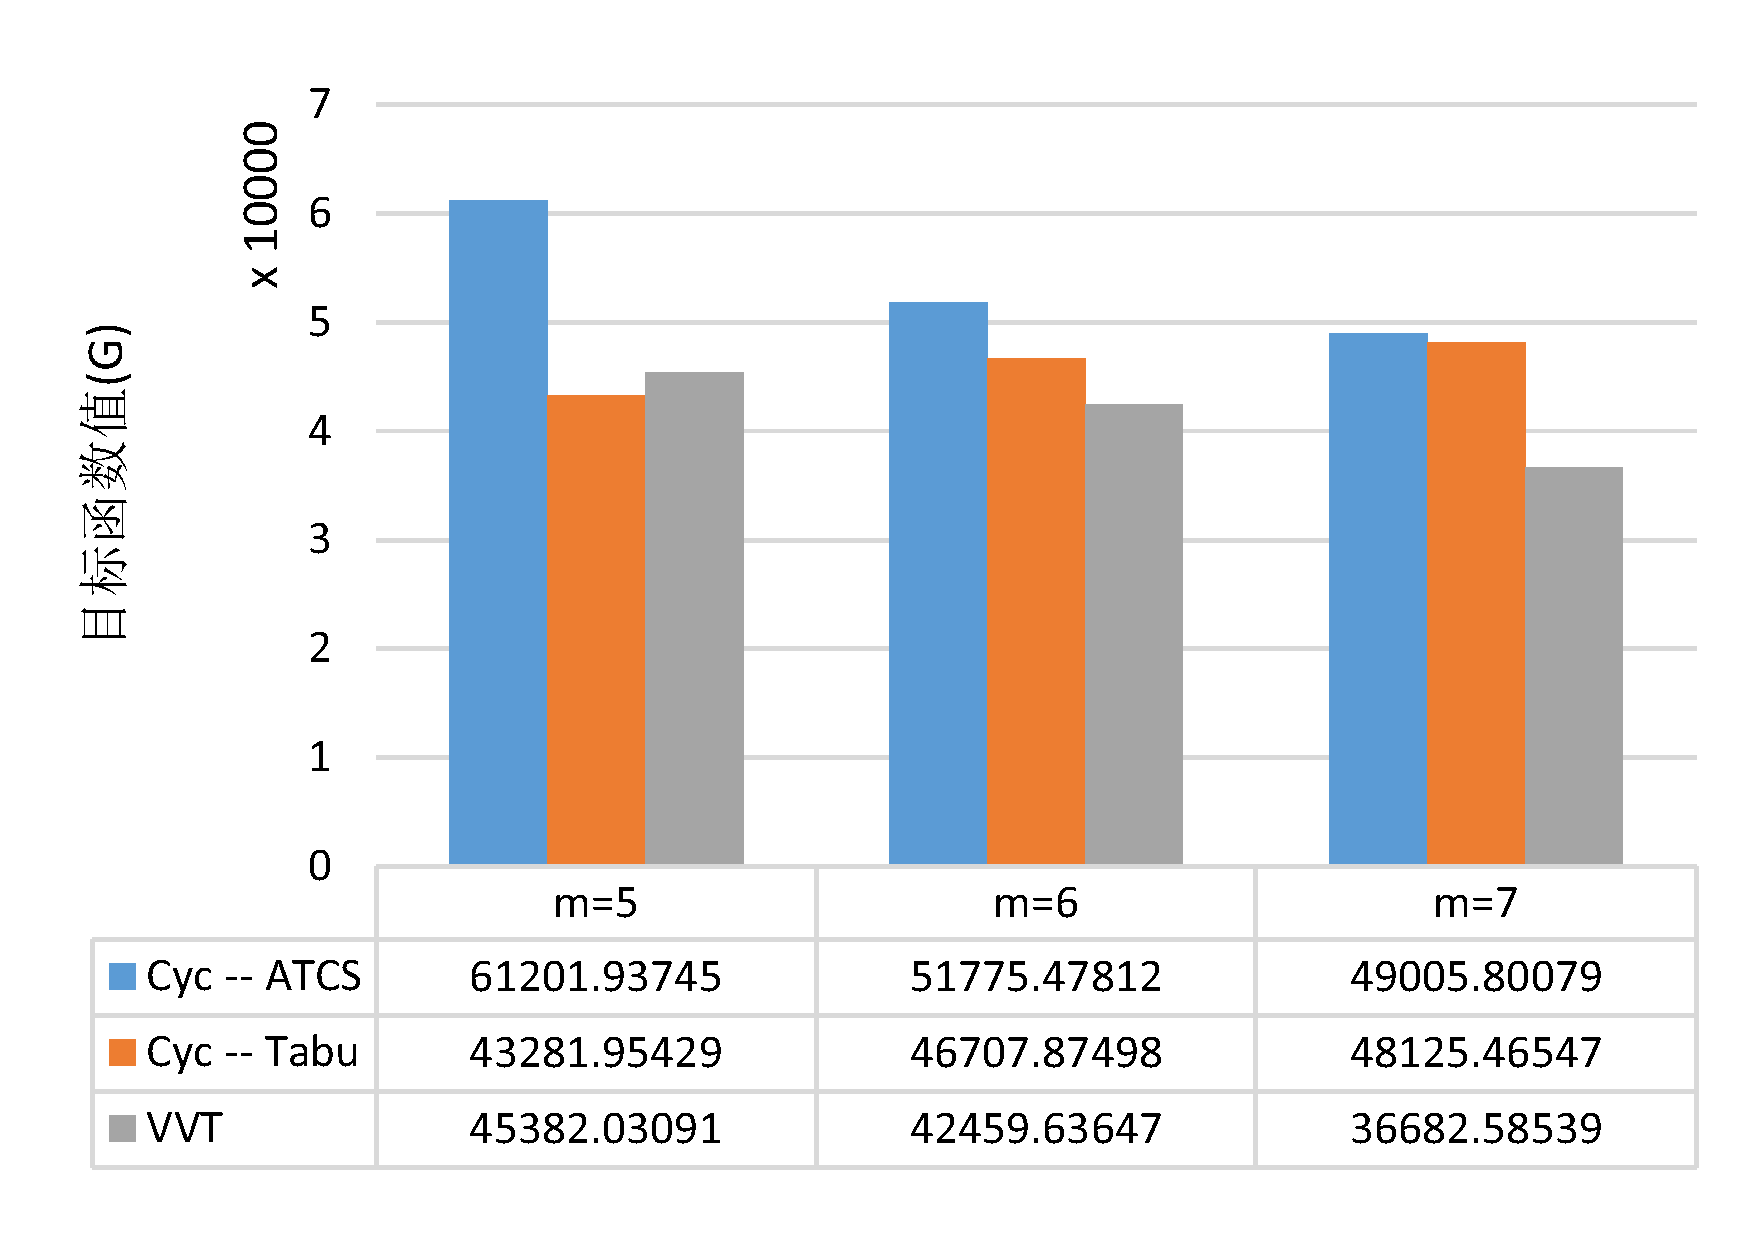
\includegraphics[height = 6cm, angle = -90]{continue_05_70}}\\
\subfloat[$n = 100$]{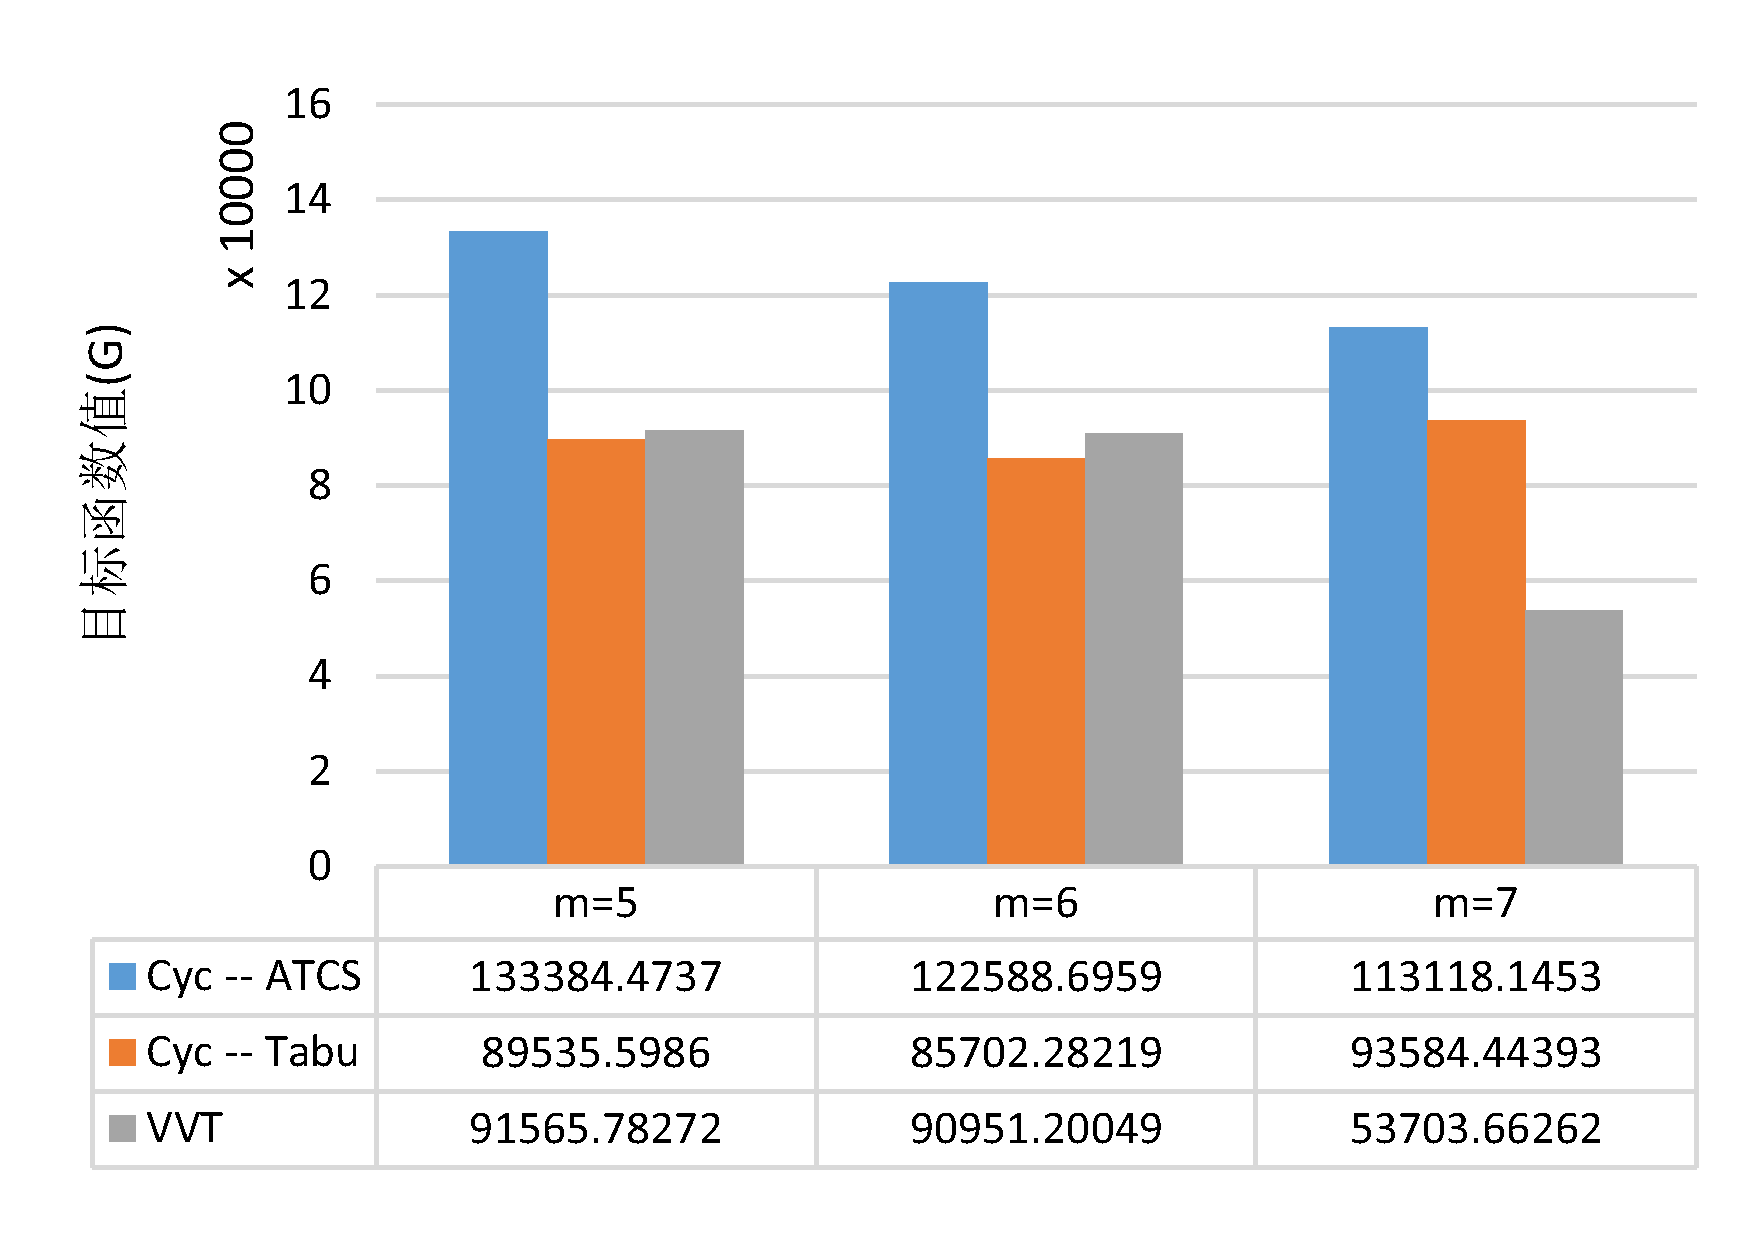
\includegraphics[height = 6cm, angle = -90]{continue_05_100}}
\subfloat[$n = 150$]{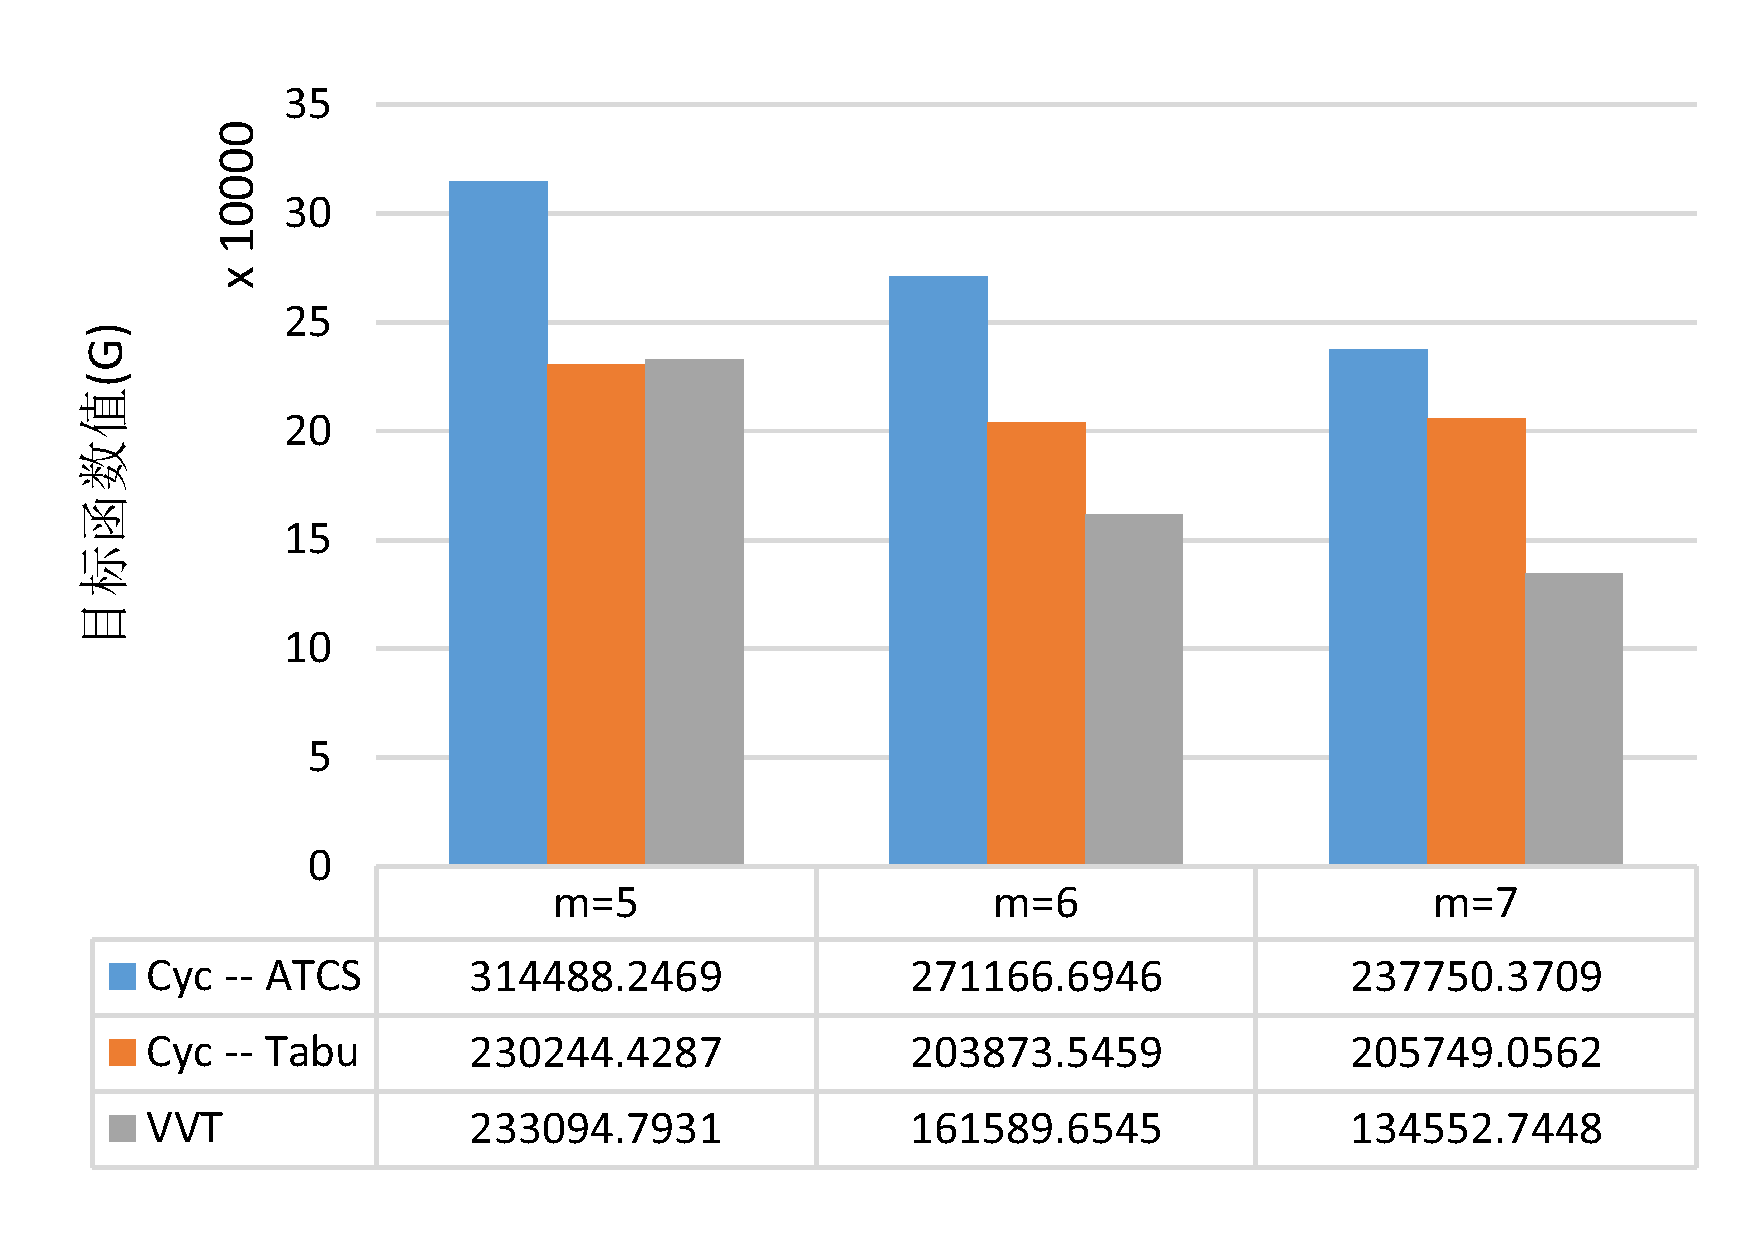
\includegraphics[height = 6cm, angle = -90]{continue_05_150}}
\subfloat[$n = 200$]{\includegraphics[height = 6cm, angle = -90]{continue_05_200}}
\subfloat[$n = 300$]{\includegraphics[height = 6cm, angle = -90]{continue_05_300}}\\
\subfloat[$n = 500$]{\includegraphics[height = 6cm, angle = -90]{continue_05_500}}
\subfloat[$n = 750$]{\includegraphics[height = 6cm, angle = -90]{continue_05_750}}
\subfloat[$n = 1000$]{\includegraphics[height = 6cm, angle = -90]{continue_05_1000}}
\caption{\label{fig:result5}模型$2$的Cyc -- ATCS、Cyc -- Tabu、VVT 算法求解目标函数值比较$(\lambda_1 = 0.5)$}
\end{sidewaysfigure}

\begin{sidewaysfigure}
\centering
\subfloat[$n = 20$]{\includegraphics[height = 6cm, angle = -90]{continue_06_20}}
\subfloat[$n = 30$]{\includegraphics[height = 6cm, angle = -90]{continue_06_300}}
\subfloat[$n = 50$]{\includegraphics[height = 6cm, angle = -90]{continue_06_50}}
\subfloat[$n = 70$]{\includegraphics[height = 6cm, angle = -90]{continue_06_70}}\\
\subfloat[$n = 100$]{\includegraphics[height = 6cm, angle = -90]{continue_06_100}}
\subfloat[$n = 150$]{\includegraphics[height = 6cm, angle = -90]{continue_06_150}}
\subfloat[$n = 200$]{\includegraphics[height = 6cm, angle = -90]{continue_06_200}}
\subfloat[$n = 300$]{\includegraphics[height = 6cm, angle = -90]{continue_06_300}}\\
\subfloat[$n = 500$]{\includegraphics[height = 6cm, angle = -90]{continue_06_500}}
\subfloat[$n = 750$]{\includegraphics[height = 6cm, angle = -90]{continue_06_750}}
\subfloat[$n = 1000$]{\includegraphics[height = 6cm, angle = -90]{continue_06_1000}}
\caption{\label{fig:result6}模型$2$的Cyc -- ATCS、Cyc -- Tabu、VVT 算法求解目标函数值比较$(\lambda_1 = 0.6)$}
\end{sidewaysfigure}

\begin{sidewaysfigure}
\centering
\subfloat[$n = 20$]{\includegraphics[height = 6cm, angle = -90]{Rb_04_20}}
\subfloat[$n = 30$]{\includegraphics[height = 6cm, angle = -90]{Rb_04_300}}
\subfloat[$n = 50$]{\includegraphics[height = 6cm, angle = -90]{Rb_04_50}}
\subfloat[$n = 70$]{\includegraphics[height = 6cm, angle = -90]{Rb_04_70}}\\
\subfloat[$n = 100$]{\includegraphics[height = 6cm, angle = -90]{Rb_04_100}}
\subfloat[$n = 150$]{\includegraphics[height = 6cm, angle = -90]{Rb_04_150}}
\subfloat[$n = 200$]{\includegraphics[height = 6cm, angle = -90]{Rb_04_200}}
\subfloat[$n = 300$]{\includegraphics[height = 6cm, angle = -90]{Rb_04_300}}\\
\subfloat[$n = 500$]{\includegraphics[height = 6cm, angle = -90]{Rb_04_500}}
\subfloat[$n = 750$]{\includegraphics[height = 6cm, angle = -90]{Rb_04_750}}
\subfloat[$n = 1000$]{\includegraphics[height = 6cm, angle = -90]{Rb_04_1000}}
\caption{\label{fig:result7}模型$2$的Cyc -- ATCS、Cyc -- Tabu、VVT 算法求解流水线均衡率比较$(\lambda_1 = 0.4)$}
\end{sidewaysfigure}

\begin{sidewaysfigure}
\centering
\subfloat[$n = 20$]{\includegraphics[height = 6cm, angle = -90]{Rb_05_20}}
\subfloat[$n = 30$]{\includegraphics[height = 6cm, angle = -90]{Rb_05_300}}
\subfloat[$n = 50$]{\includegraphics[height = 6cm, angle = -90]{Rb_05_50}}
\subfloat[$n = 70$]{\includegraphics[height = 6cm, angle = -90]{Rb_05_70}}\\
\subfloat[$n = 100$]{\includegraphics[height = 6cm, angle = -90]{Rb_05_100}}
\subfloat[$n = 150$]{\includegraphics[height = 6cm, angle = -90]{Rb_05_150}}
\subfloat[$n = 200$]{\includegraphics[height = 6cm, angle = -90]{Rb_05_200}}
\subfloat[$n = 300$]{\includegraphics[height = 6cm, angle = -90]{Rb_05_300}}\\
\subfloat[$n = 500$]{\includegraphics[height = 6cm, angle = -90]{Rb_05_500}}
\subfloat[$n = 750$]{\includegraphics[height = 6cm, angle = -90]{Rb_05_750}}
\subfloat[$n = 1000$]{\includegraphics[height = 6cm, angle = -90]{Rb_05_1000}}
\caption{\label{fig:result8}模型$2$的Cyc -- ATCS、Cyc -- Tabu、VVT 算法求解流水线均衡率比较$(\lambda_1 = 0.5)$}
\end{sidewaysfigure}

\begin{sidewaysfigure}
\centering
\subfloat[$n = 20$]{\includegraphics[height = 6cm, angle = -90]{Rb_06_20}}
\subfloat[$n = 30$]{\includegraphics[height = 6cm, angle = -90]{Rb_06_300}}
\subfloat[$n = 50$]{\includegraphics[height = 6cm, angle = -90]{Rb_06_50}}
\subfloat[$n = 70$]{\includegraphics[height = 6cm, angle = -90]{Rb_06_70}}\\
\subfloat[$n = 100$]{\includegraphics[height = 6cm, angle = -90]{Rb_06_100}}
\subfloat[$n = 150$]{\includegraphics[height = 6cm, angle = -90]{Rb_06_150}}
\subfloat[$n = 200$]{\includegraphics[height = 6cm, angle = -90]{Rb_06_200}}
\subfloat[$n = 300$]{\includegraphics[height = 6cm, angle = -90]{Rb_06_300}}\\
\subfloat[$n = 500$]{\includegraphics[height = 6cm, angle = -90]{Rb_06_500}}
\subfloat[$n = 750$]{\includegraphics[height = 6cm, angle = -90]{Rb_06_750}}
\subfloat[$n = 1000$]{\includegraphics[height = 6cm, angle = -90]{Rb_06_1000}}
\caption{\label{fig:result9}模型$2$的Cyc -- ATCS、Cyc -- Tabu、VVT 算法求解流水线均衡率比较$(\lambda_1 = 0.6)$}
\end{sidewaysfigure}
\chapter{算法代码}
\begin{asparaenum}
\item experiment\_data.py
\end{asparaenum}
\lstset{	basicstyle = \tiny\ttfamily,
	keywordstyle = \color{blue}\bfseries,
	stringstyle = \color{red},
	emph = {solve},
	emphstyle = \color{Green}\bfseries,
	commentstyle = \color{CadetBlue}
	}
\begin{lstlisting}[language = Python]
import sys
sys.path.append(".\\functions")
import generate
from collections import namedtuple
Item = namedtuple("Item", ['process','due','wt','wc'])

def  h(lambda1,lambda2,tardiness,completion,wt,wc):			# define the contribution of one item for the obj function
	value = lambda1*wt*tardiness + lambda2*wc*completion
	return value

def solve(input_data):
	Data = input_data.split('\n')					# load data
	n = len(Data) -1						# get the amount of items
	print n
	items = []
	for j in xrange(n):
		data = Data[j]
		parts = data.split()
		p = int(parts[0])					# get the process time
		s = int(parts[2])						# get the setup time
		d = int(parts[3])					# get the due date
		wt = int(parts[4])					# get the tardiness weights
		wc = int(parts[5])					# get the completion weights
		items.append(Item(p+s,d,wt,wc))			# combine those item data
	print 'Data loaded!'
	J = range(n)
	m = 5
	S = []
	a = []
	tl = []
	L = []
	c = [None]*n
	for l in xrange(m):
		S.append([])
		a.append(0)
		tl.append(0)
	t = 0
	f = open(".\\result\\sky",'w')
	while J:
		if 0 in a:
			l_star = a.index(0)
			p,d,wt = [],[],[]
			for j in J:				
				item = items[j]
				p.append(item.process)
				d.append(item.due)
				wt.append(item.wt)
			orderidx = generate.Idx(t,p,d,wt)
			j_star = J[orderidx.index(max(orderidx))]
			S[l_star].append(j_star)
			J.remove(j_star)
			L.append(j_star)
			tl[l_star] = t + items[j_star].process
			c[j_star] = tl[l_star]
			a[l_star] = 1
		else:
			t_star = min(tl)
			for l in xrange(m):
				if tl[l] == t_star:
					a[l] = 0
			t = t_star
	print 'initial sloution done!'
	f.write(str(S) + '\n' + str(L) + '\n' + str(c))
	f.close()


import sys
if __name__ == '__main__':
	if len(sys.argv) > 1:
		file_location = sys.argv[1].strip()
#		output = sys.argv[2].strip()
		input_data_file = open(file_location, 'r')
		input_data = ''.join(input_data_file.readlines())
		input_data_file.close()
		solve(input_data)
\end{lstlisting}
\section{456456}
\addcontentsline{toc}{section}{附录1 毕业设计文献综述}
\addcontentsline{toc}{section}{附录2 毕业设计开题报告}
\addcontentsline{toc}{section}{附录3 毕业设计外文翻译(中文译文与外文原文)}
\hspace*{7.0mm}
\hspace*{4.0mm}
\begin{minipage}[t]{95mm}
    \songti\bfseries{
    \sectionmark{附录1 毕业设计文献综述}
    附录1 毕业设计文献综述

    \vspace*{7.0mm}

    \sectionmark{附录2 毕业设计开题报告}
    附录2 毕业设计开题报告

    \vspace*{7.0mm}

    \sectionmark{附录3 毕业设计外文翻译(中文译文与外文原文)}
    附录3 毕业设计外文翻译(中文译文与外文原文)}
\end{minipage}
